% This example is meant to be compiled with lualatex or xelatex
% The theme itself also supports pdflatex
\PassOptionsToPackage{unicode}{hyperref}
\documentclass[aspectratio=169, 12pt]{beamer}

% Load packages you need here
\usepackage{polyglossia}
\setmainlanguage{german}

\usepackage{csquotes}
    

\usepackage{amsmath}
\usepackage{amssymb}
\usepackage{mathtools}

\usepackage{hyperref}
\usepackage{bookmark}

\usepackage{graphicx}
\usepackage{wrapfig}

\usepackage[utf8]{inputenc}
\usepackage{pgfplots}
% \DeclareUnicodeCharacter{2212}{−}
\usepgfplotslibrary{groupplots,dateplot}
\usetikzlibrary{patterns,shapes.arrows}
\pgfplotsset{
  compat=newest,
  legend style={
    font=\scriptsize,
  },
  x tick label style={
    font=\scriptsize,
    /pgf/number format/.cd,
    use comma,
    % fixed,
    % fixed zerofill,
    % precision=1,
    /tikz/.cd
  },
  y tick label style={
    font=\scriptsize,
    /pgf/number format/.cd,
    use comma,
    fixed,
    fixed zerofill,
    precision=1,
    /tikz/.cd
  },
  x label style={font=\footnotesize},
  y label style={font=\footnotesize}
}
% \pgfplotsset{compat=newest}

% load the theme after all packages

\usetheme[
  showtotalframes, % show total number of frames in the footline
]{tudo}

\setbeamertemplate{section in toc}[sections numbered]

% Put settings here, like
\unimathsetup{
  math-style=ISO,
  bold-style=ISO,
  nabla=upright,
  partial=upright,
  mathrm=sym,
}
\setmathfont[range={\mathcal,\mathbfcal},StylisticSet=1]{XITS Math}

% Tikz
\usepackage{tikz}
\usetikzlibrary{shapes,arrows}

\title{Kompression neuronaler Netze mit Hilfe von Wavelet Transformationen}
\author[L.~Camphausen]{Lucas Camphausen}
\date{6. September 2022}
\institute[LS 11]{Lehrstuhl für Algorithm Engineering (LS 11) \\  Fakultät für Informatik \\~\\ Betreuer: Prof. Dr. Rudolph, Dr.-Ing. Brehler (Fraunhofer IML)}
% \betreuer{Prof. Dr. Rudolph, Dr. Marius Brehler (Fraunhofer IML)}
% \titlegraphic{\includegraphics[height=4.3cm]{example-image-a}}


\begin{document}

\begin{tiny}
  \maketitle
\end{tiny}

% --- Übersicht
\begin{frame}{Übersicht}
  \tableofcontents
\end{frame}
% --- Übersicht

% === Motivation
\section{Motivation}

\begin{frame}{Übersicht}
  \tableofcontents[currentsection]
\end{frame}

% --- Motivation 1
\begin{frame}{Motivation}
  \begin{itemize}
    \item Convolutional Neural Networks (CNN) sind ein vielfach genutztes Konzept des Maschinellen Lernens.
    \item Speicherbedarf ist verhältnismäßig groß:
          \begin{itemize}
            \item VGG16: 520 MB
            \item ResNet18: 40 MB
            \item MobileNet v2: 16 MB
          \end{itemize}
    \item Ausführung auf ressourcenbeschränkter Hardware problematisch:
          \begin{itemize}
            \item Teils stehen nur wenige MB Flash zur Verfügung.
            \item Ressourcenverbrauch (insb. Speicherbedarf) muss gesenkt werden.
          \end{itemize}
  \end{itemize}
\end{frame}
% --- Motivation 1

% === Motivation

% === Stand der Forschung
\section{Stand der Forschung}

\begin{frame}{Übersicht}
  \tableofcontents[currentsection]
\end{frame}

% --- Stand der Forschung 1
\begin{frame}{Stand der Forschung}
  Verschiedene Techniken zur Kompression stehen zur Verfügung:

  \begin{itemize}
    \item Quantisierung
          \begin{itemize}
            \item Reduzierung des Speicherbedarfs der einzelnen Parameter
            \item Repräsentation der Parameter mit geringerer Genauigkeit (16-bit Gleitkommazahl, 8-bit Ganzzahl, Boolean)
          \end{itemize}
    \item Pruning
          \begin{itemize}
            \item Reduzierung der Anzahl an Parametern
            \item Unstrukturiertes Entfernen einzelner unwichtiger Parameter
            \item Strukturiertes Entfernen von Filtern
          \end{itemize}
  \end{itemize}
\end{frame}
% --- Stand der Forschung 1

% --- Stand der Forschung 2
\begin{frame}
  \begin{itemize}
    \item Weight-Sharing
          \begin{itemize}
            \item Ausnutzen von Ähnlichkeiten zwischen Filtern
            \item Clustering von Filtern
            \item Speicherung der Clusterzentren
          \end{itemize}
    \item Transformationsbasierte Kompression
          \begin{itemize}
            \item Parallelen zur Kompression von Bilddaten
            \item Transformation der Daten in andere Repräsentation:
                  \begin{itemize}
                    \item JPEG (Diskrete Kosinus Transformation)
                    \item JPEG 2000 (Diskrete Wavelet Transformation)
                  \end{itemize}
            \item Vernachlässigung von unwichtigen Koeffizienten
          \end{itemize}
  \end{itemize}
\end{frame}
% --- Stand der Forschung 2

% === Grundlagen
\section{Transformationsbasierte Kompression}

\begin{frame}{Übersicht}
  \tableofcontents[currentsection]
\end{frame}

\begin{frame}{Ziel der Arbeit}
  Ziel der Arbeit ist die Untersuchung der Möglichkeiten neuronale Netze mit Hilfe der Diskreten Wavelet Transformation zu komprimieren.
  Folgende Aspekte sollen betrachtet werden:
  \begin{itemize}
    \item Wie lässt sich durch die DWT eine Kompression erreichen?
    \item Welche Kompressionsraten können erreicht werden?
    \item Ist es möglich das Netz auf einem Mikrocontroller bare-metal ohne Betriebssystem auszuführen?
    \item Genauigkeit und Laufzeit sind nicht immer die kritischen Messgrößen.
    \item Es soll mit der DCT verglichen werden.
  \end{itemize}
\end{frame}

% --- Grundlagen 1
% \begin{frame}{Grundlagen}
%   Die Gewichte, vor allem die der Faltungsschichten, sollen auf folgende Art komprimiert werden:
%   \begin{itemize}
%     \item Filter werden in Blöcken gruppiert.
%           \begin{itemize}
%             \item Im einfachsten Fall bildet jeder Filter einen eigenen Block.
%           \end{itemize}
%     \item Blöcke werden mit der DWT transformiert.
%     \item Für jedes Subband wird ein Clustering mit verschiedenen Parametern durchgeführt.
%     \item Clusterzentren werden gespeichert.
%     \item Das Netz wird nachtrainiert.
%   \end{itemize}
% \end{frame}
% --- Grundlagen 1

% --- Grundlagen 2
\begin{frame}{Vorgehen}
  \vspace{-0.8cm}
  \begin{center}
    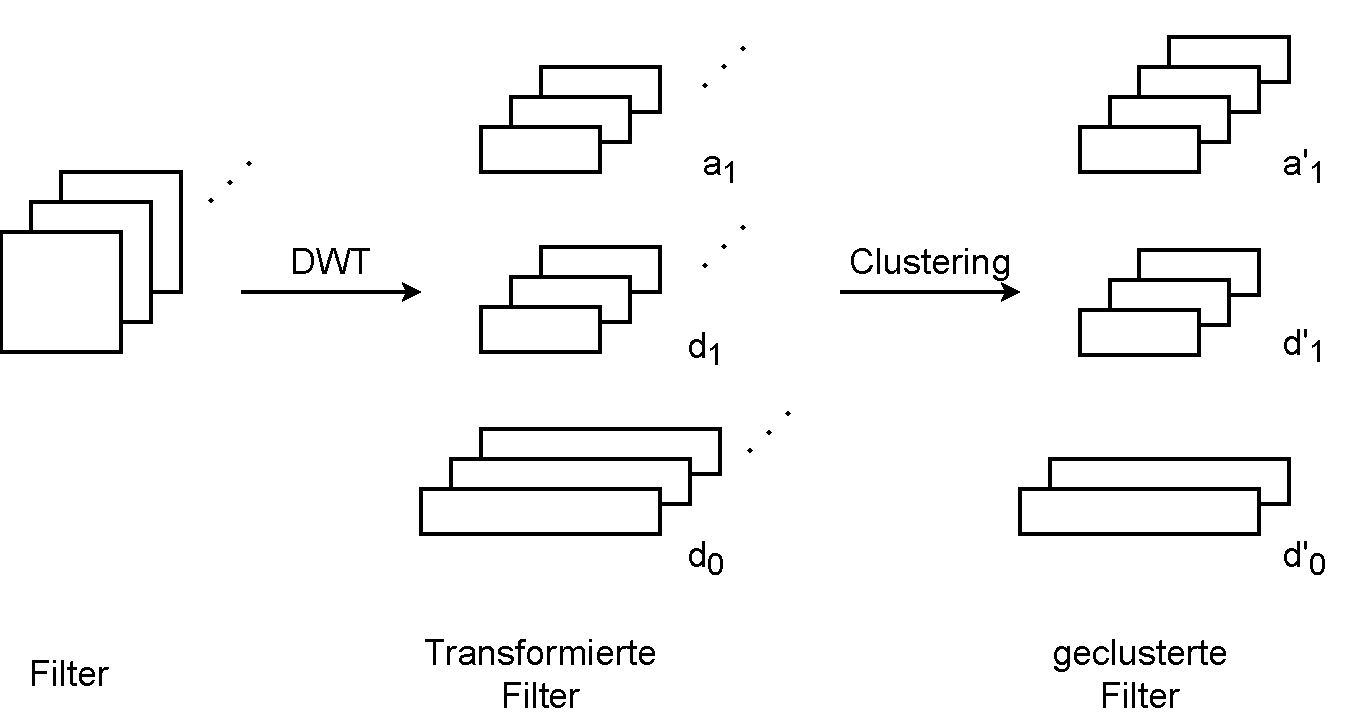
\includegraphics[height=5.5cm]{images/Vorgehen2.pdf}
  \end{center}
\end{frame}
% --- Grundlagen 2

% --- DCT 1
\begin{frame}{Diskrete Kosinus Transformation (DCT)}
  \begin{itemize}
    \item DCT ist eine Transformation aus dem Orts- in den Frequenzbereich.
    \item Eingangssignal wird als Linearkombination von Kosinusfunktionen verschiedener Frequenzen dargestellt.
    \item Datenpunkte $x_0, ..., x_{N-1}$ sind gegeben.
    \item DCT Koeffizienten $u_0, ..., u_{N-1}$ werden wie folgt berechnet:
          \begin{equation*}
            u_k = \sum_{n=0}^{N-1} x_n d_k(n) \coloneqq \sum_{n=0}^{N-1} x_n cos\left( \frac{\pi}{N} k \left( n + \frac{1}{2} \right) \right), \qquad k = 0, ..., N-1
          \end{equation*}
  \end{itemize}
\end{frame}
% --- DCT 1

% --- DCT 2
\begin{frame}{DCT Basisfunktionen}
  \begin{wrapfigure}{l}{8cm}
    \vspace{-1.2cm}
    \resizebox{7.5cm}{!}{%
      % This file was created with tikzplotlib v0.10.1.
\begin{tikzpicture}

\definecolor{crimson2143940}{RGB}{214,39,40}
\definecolor{darkgray176}{RGB}{176,176,176}
\definecolor{darkorange25512714}{RGB}{255,127,14}
\definecolor{forestgreen4416044}{RGB}{44,160,44}
\definecolor{lightgray204}{RGB}{204,204,204}
\definecolor{steelblue31119180}{RGB}{31,119,180}

\begin{axis}[
legend cell align={left},
legend style={
  fill opacity=0.8,
  draw opacity=1,
  text opacity=1,
  at={(0.03,0.03)},
  anchor=south west,
  draw=lightgray204
},
tick align=outside,
tick pos=left,
x grid style={darkgray176},
xlabel={\(\displaystyle x\)},
xmin=-0.4, xmax=8.4,
xtick style={color=black},
y grid style={darkgray176},
ylabel={\(\displaystyle d_k(x)\)},
ymin=-1.09999991887624, ymax=1.09999999613696,
ytick style={color=black}
]
\addplot [semithick, steelblue31119180]
table {%
0 1
0.00800800800800801 1
0.016016016016016 1
0.024024024024024 1
0.032032032032032 1
0.04004004004004 1
0.048048048048048 1
0.0560560560560561 1
0.0640640640640641 1
0.0720720720720721 1
0.0800800800800801 1
0.0880880880880881 1
0.0960960960960961 1
0.104104104104104 1
0.112112112112112 1
0.12012012012012 1
0.128128128128128 1
0.136136136136136 1
0.144144144144144 1
0.152152152152152 1
0.16016016016016 1
0.168168168168168 1
0.176176176176176 1
0.184184184184184 1
0.192192192192192 1
0.2002002002002 1
0.208208208208208 1
0.216216216216216 1
0.224224224224224 1
0.232232232232232 1
0.24024024024024 1
0.248248248248248 1
0.256256256256256 1
0.264264264264264 1
0.272272272272272 1
0.28028028028028 1
0.288288288288288 1
0.296296296296296 1
0.304304304304304 1
0.312312312312312 1
0.32032032032032 1
0.328328328328328 1
0.336336336336336 1
0.344344344344344 1
0.352352352352352 1
0.36036036036036 1
0.368368368368368 1
0.376376376376376 1
0.384384384384384 1
0.392392392392392 1
0.4004004004004 1
0.408408408408408 1
0.416416416416416 1
0.424424424424424 1
0.432432432432432 1
0.44044044044044 1
0.448448448448448 1
0.456456456456456 1
0.464464464464464 1
0.472472472472472 1
0.48048048048048 1
0.488488488488488 1
0.496496496496497 1
0.504504504504504 1
0.512512512512513 1
0.520520520520521 1
0.528528528528528 1
0.536536536536537 1
0.544544544544544 1
0.552552552552553 1
0.560560560560561 1
0.568568568568569 1
0.576576576576577 1
0.584584584584585 1
0.592592592592593 1
0.600600600600601 1
0.608608608608609 1
0.616616616616617 1
0.624624624624625 1
0.632632632632633 1
0.640640640640641 1
0.648648648648649 1
0.656656656656657 1
0.664664664664665 1
0.672672672672673 1
0.680680680680681 1
0.688688688688689 1
0.696696696696697 1
0.704704704704705 1
0.712712712712713 1
0.720720720720721 1
0.728728728728729 1
0.736736736736737 1
0.744744744744745 1
0.752752752752753 1
0.760760760760761 1
0.768768768768769 1
0.776776776776777 1
0.784784784784785 1
0.792792792792793 1
0.800800800800801 1
0.808808808808809 1
0.816816816816817 1
0.824824824824825 1
0.832832832832833 1
0.840840840840841 1
0.848848848848849 1
0.856856856856857 1
0.864864864864865 1
0.872872872872873 1
0.880880880880881 1
0.888888888888889 1
0.896896896896897 1
0.904904904904905 1
0.912912912912913 1
0.920920920920921 1
0.928928928928929 1
0.936936936936937 1
0.944944944944945 1
0.952952952952953 1
0.960960960960961 1
0.968968968968969 1
0.976976976976977 1
0.984984984984985 1
0.992992992992993 1
1.001001001001 1
1.00900900900901 1
1.01701701701702 1
1.02502502502503 1
1.03303303303303 1
1.04104104104104 1
1.04904904904905 1
1.05705705705706 1
1.06506506506507 1
1.07307307307307 1
1.08108108108108 1
1.08908908908909 1
1.0970970970971 1
1.10510510510511 1
1.11311311311311 1
1.12112112112112 1
1.12912912912913 1
1.13713713713714 1
1.14514514514515 1
1.15315315315315 1
1.16116116116116 1
1.16916916916917 1
1.17717717717718 1
1.18518518518519 1
1.19319319319319 1
1.2012012012012 1
1.20920920920921 1
1.21721721721722 1
1.22522522522523 1
1.23323323323323 1
1.24124124124124 1
1.24924924924925 1
1.25725725725726 1
1.26526526526527 1
1.27327327327327 1
1.28128128128128 1
1.28928928928929 1
1.2972972972973 1
1.30530530530531 1
1.31331331331331 1
1.32132132132132 1
1.32932932932933 1
1.33733733733734 1
1.34534534534535 1
1.35335335335335 1
1.36136136136136 1
1.36936936936937 1
1.37737737737738 1
1.38538538538539 1
1.39339339339339 1
1.4014014014014 1
1.40940940940941 1
1.41741741741742 1
1.42542542542543 1
1.43343343343343 1
1.44144144144144 1
1.44944944944945 1
1.45745745745746 1
1.46546546546547 1
1.47347347347347 1
1.48148148148148 1
1.48948948948949 1
1.4974974974975 1
1.50550550550551 1
1.51351351351351 1
1.52152152152152 1
1.52952952952953 1
1.53753753753754 1
1.54554554554555 1
1.55355355355355 1
1.56156156156156 1
1.56956956956957 1
1.57757757757758 1
1.58558558558559 1
1.59359359359359 1
1.6016016016016 1
1.60960960960961 1
1.61761761761762 1
1.62562562562563 1
1.63363363363363 1
1.64164164164164 1
1.64964964964965 1
1.65765765765766 1
1.66566566566567 1
1.67367367367367 1
1.68168168168168 1
1.68968968968969 1
1.6976976976977 1
1.70570570570571 1
1.71371371371371 1
1.72172172172172 1
1.72972972972973 1
1.73773773773774 1
1.74574574574575 1
1.75375375375375 1
1.76176176176176 1
1.76976976976977 1
1.77777777777778 1
1.78578578578579 1
1.79379379379379 1
1.8018018018018 1
1.80980980980981 1
1.81781781781782 1
1.82582582582583 1
1.83383383383383 1
1.84184184184184 1
1.84984984984985 1
1.85785785785786 1
1.86586586586587 1
1.87387387387387 1
1.88188188188188 1
1.88988988988989 1
1.8978978978979 1
1.90590590590591 1
1.91391391391391 1
1.92192192192192 1
1.92992992992993 1
1.93793793793794 1
1.94594594594595 1
1.95395395395395 1
1.96196196196196 1
1.96996996996997 1
1.97797797797798 1
1.98598598598599 1
1.99399399399399 1
2.002002002002 1
2.01001001001001 1
2.01801801801802 1
2.02602602602603 1
2.03403403403403 1
2.04204204204204 1
2.05005005005005 1
2.05805805805806 1
2.06606606606607 1
2.07407407407407 1
2.08208208208208 1
2.09009009009009 1
2.0980980980981 1
2.10610610610611 1
2.11411411411411 1
2.12212212212212 1
2.13013013013013 1
2.13813813813814 1
2.14614614614615 1
2.15415415415415 1
2.16216216216216 1
2.17017017017017 1
2.17817817817818 1
2.18618618618619 1
2.19419419419419 1
2.2022022022022 1
2.21021021021021 1
2.21821821821822 1
2.22622622622623 1
2.23423423423423 1
2.24224224224224 1
2.25025025025025 1
2.25825825825826 1
2.26626626626627 1
2.27427427427427 1
2.28228228228228 1
2.29029029029029 1
2.2982982982983 1
2.30630630630631 1
2.31431431431431 1
2.32232232232232 1
2.33033033033033 1
2.33833833833834 1
2.34634634634635 1
2.35435435435435 1
2.36236236236236 1
2.37037037037037 1
2.37837837837838 1
2.38638638638639 1
2.39439439439439 1
2.4024024024024 1
2.41041041041041 1
2.41841841841842 1
2.42642642642643 1
2.43443443443443 1
2.44244244244244 1
2.45045045045045 1
2.45845845845846 1
2.46646646646647 1
2.47447447447447 1
2.48248248248248 1
2.49049049049049 1
2.4984984984985 1
2.50650650650651 1
2.51451451451451 1
2.52252252252252 1
2.53053053053053 1
2.53853853853854 1
2.54654654654655 1
2.55455455455455 1
2.56256256256256 1
2.57057057057057 1
2.57857857857858 1
2.58658658658659 1
2.59459459459459 1
2.6026026026026 1
2.61061061061061 1
2.61861861861862 1
2.62662662662663 1
2.63463463463463 1
2.64264264264264 1
2.65065065065065 1
2.65865865865866 1
2.66666666666667 1
2.67467467467467 1
2.68268268268268 1
2.69069069069069 1
2.6986986986987 1
2.70670670670671 1
2.71471471471471 1
2.72272272272272 1
2.73073073073073 1
2.73873873873874 1
2.74674674674675 1
2.75475475475475 1
2.76276276276276 1
2.77077077077077 1
2.77877877877878 1
2.78678678678679 1
2.79479479479479 1
2.8028028028028 1
2.81081081081081 1
2.81881881881882 1
2.82682682682683 1
2.83483483483483 1
2.84284284284284 1
2.85085085085085 1
2.85885885885886 1
2.86686686686687 1
2.87487487487487 1
2.88288288288288 1
2.89089089089089 1
2.8988988988989 1
2.90690690690691 1
2.91491491491491 1
2.92292292292292 1
2.93093093093093 1
2.93893893893894 1
2.94694694694695 1
2.95495495495495 1
2.96296296296296 1
2.97097097097097 1
2.97897897897898 1
2.98698698698699 1
2.99499499499499 1
3.003003003003 1
3.01101101101101 1
3.01901901901902 1
3.02702702702703 1
3.03503503503504 1
3.04304304304304 1
3.05105105105105 1
3.05905905905906 1
3.06706706706707 1
3.07507507507508 1
3.08308308308308 1
3.09109109109109 1
3.0990990990991 1
3.10710710710711 1
3.11511511511512 1
3.12312312312312 1
3.13113113113113 1
3.13913913913914 1
3.14714714714715 1
3.15515515515516 1
3.16316316316316 1
3.17117117117117 1
3.17917917917918 1
3.18718718718719 1
3.1951951951952 1
3.2032032032032 1
3.21121121121121 1
3.21921921921922 1
3.22722722722723 1
3.23523523523524 1
3.24324324324324 1
3.25125125125125 1
3.25925925925926 1
3.26726726726727 1
3.27527527527528 1
3.28328328328328 1
3.29129129129129 1
3.2992992992993 1
3.30730730730731 1
3.31531531531532 1
3.32332332332332 1
3.33133133133133 1
3.33933933933934 1
3.34734734734735 1
3.35535535535536 1
3.36336336336336 1
3.37137137137137 1
3.37937937937938 1
3.38738738738739 1
3.3953953953954 1
3.4034034034034 1
3.41141141141141 1
3.41941941941942 1
3.42742742742743 1
3.43543543543544 1
3.44344344344344 1
3.45145145145145 1
3.45945945945946 1
3.46746746746747 1
3.47547547547548 1
3.48348348348348 1
3.49149149149149 1
3.4994994994995 1
3.50750750750751 1
3.51551551551552 1
3.52352352352352 1
3.53153153153153 1
3.53953953953954 1
3.54754754754755 1
3.55555555555556 1
3.56356356356356 1
3.57157157157157 1
3.57957957957958 1
3.58758758758759 1
3.5955955955956 1
3.6036036036036 1
3.61161161161161 1
3.61961961961962 1
3.62762762762763 1
3.63563563563564 1
3.64364364364364 1
3.65165165165165 1
3.65965965965966 1
3.66766766766767 1
3.67567567567568 1
3.68368368368368 1
3.69169169169169 1
3.6996996996997 1
3.70770770770771 1
3.71571571571572 1
3.72372372372372 1
3.73173173173173 1
3.73973973973974 1
3.74774774774775 1
3.75575575575576 1
3.76376376376376 1
3.77177177177177 1
3.77977977977978 1
3.78778778778779 1
3.7957957957958 1
3.8038038038038 1
3.81181181181181 1
3.81981981981982 1
3.82782782782783 1
3.83583583583584 1
3.84384384384384 1
3.85185185185185 1
3.85985985985986 1
3.86786786786787 1
3.87587587587588 1
3.88388388388388 1
3.89189189189189 1
3.8998998998999 1
3.90790790790791 1
3.91591591591592 1
3.92392392392392 1
3.93193193193193 1
3.93993993993994 1
3.94794794794795 1
3.95595595595596 1
3.96396396396396 1
3.97197197197197 1
3.97997997997998 1
3.98798798798799 1
3.995995995996 1
4.004004004004 1
4.01201201201201 1
4.02002002002002 1
4.02802802802803 1
4.03603603603604 1
4.04404404404404 1
4.05205205205205 1
4.06006006006006 1
4.06806806806807 1
4.07607607607608 1
4.08408408408408 1
4.09209209209209 1
4.1001001001001 1
4.10810810810811 1
4.11611611611612 1
4.12412412412412 1
4.13213213213213 1
4.14014014014014 1
4.14814814814815 1
4.15615615615616 1
4.16416416416416 1
4.17217217217217 1
4.18018018018018 1
4.18818818818819 1
4.1961961961962 1
4.2042042042042 1
4.21221221221221 1
4.22022022022022 1
4.22822822822823 1
4.23623623623624 1
4.24424424424424 1
4.25225225225225 1
4.26026026026026 1
4.26826826826827 1
4.27627627627628 1
4.28428428428428 1
4.29229229229229 1
4.3003003003003 1
4.30830830830831 1
4.31631631631632 1
4.32432432432432 1
4.33233233233233 1
4.34034034034034 1
4.34834834834835 1
4.35635635635636 1
4.36436436436436 1
4.37237237237237 1
4.38038038038038 1
4.38838838838839 1
4.3963963963964 1
4.4044044044044 1
4.41241241241241 1
4.42042042042042 1
4.42842842842843 1
4.43643643643644 1
4.44444444444444 1
4.45245245245245 1
4.46046046046046 1
4.46846846846847 1
4.47647647647648 1
4.48448448448448 1
4.49249249249249 1
4.5005005005005 1
4.50850850850851 1
4.51651651651652 1
4.52452452452452 1
4.53253253253253 1
4.54054054054054 1
4.54854854854855 1
4.55655655655656 1
4.56456456456456 1
4.57257257257257 1
4.58058058058058 1
4.58858858858859 1
4.5965965965966 1
4.6046046046046 1
4.61261261261261 1
4.62062062062062 1
4.62862862862863 1
4.63663663663664 1
4.64464464464464 1
4.65265265265265 1
4.66066066066066 1
4.66866866866867 1
4.67667667667668 1
4.68468468468468 1
4.69269269269269 1
4.7007007007007 1
4.70870870870871 1
4.71671671671672 1
4.72472472472472 1
4.73273273273273 1
4.74074074074074 1
4.74874874874875 1
4.75675675675676 1
4.76476476476476 1
4.77277277277277 1
4.78078078078078 1
4.78878878878879 1
4.7967967967968 1
4.8048048048048 1
4.81281281281281 1
4.82082082082082 1
4.82882882882883 1
4.83683683683684 1
4.84484484484484 1
4.85285285285285 1
4.86086086086086 1
4.86886886886887 1
4.87687687687688 1
4.88488488488488 1
4.89289289289289 1
4.9009009009009 1
4.90890890890891 1
4.91691691691692 1
4.92492492492492 1
4.93293293293293 1
4.94094094094094 1
4.94894894894895 1
4.95695695695696 1
4.96496496496496 1
4.97297297297297 1
4.98098098098098 1
4.98898898898899 1
4.996996996997 1
5.00500500500501 1
5.01301301301301 1
5.02102102102102 1
5.02902902902903 1
5.03703703703704 1
5.04504504504505 1
5.05305305305305 1
5.06106106106106 1
5.06906906906907 1
5.07707707707708 1
5.08508508508509 1
5.09309309309309 1
5.1011011011011 1
5.10910910910911 1
5.11711711711712 1
5.12512512512513 1
5.13313313313313 1
5.14114114114114 1
5.14914914914915 1
5.15715715715716 1
5.16516516516517 1
5.17317317317317 1
5.18118118118118 1
5.18918918918919 1
5.1971971971972 1
5.20520520520521 1
5.21321321321321 1
5.22122122122122 1
5.22922922922923 1
5.23723723723724 1
5.24524524524525 1
5.25325325325325 1
5.26126126126126 1
5.26926926926927 1
5.27727727727728 1
5.28528528528529 1
5.29329329329329 1
5.3013013013013 1
5.30930930930931 1
5.31731731731732 1
5.32532532532533 1
5.33333333333333 1
5.34134134134134 1
5.34934934934935 1
5.35735735735736 1
5.36536536536537 1
5.37337337337337 1
5.38138138138138 1
5.38938938938939 1
5.3973973973974 1
5.40540540540541 1
5.41341341341341 1
5.42142142142142 1
5.42942942942943 1
5.43743743743744 1
5.44544544544545 1
5.45345345345345 1
5.46146146146146 1
5.46946946946947 1
5.47747747747748 1
5.48548548548549 1
5.49349349349349 1
5.5015015015015 1
5.50950950950951 1
5.51751751751752 1
5.52552552552553 1
5.53353353353353 1
5.54154154154154 1
5.54954954954955 1
5.55755755755756 1
5.56556556556557 1
5.57357357357357 1
5.58158158158158 1
5.58958958958959 1
5.5975975975976 1
5.60560560560561 1
5.61361361361361 1
5.62162162162162 1
5.62962962962963 1
5.63763763763764 1
5.64564564564565 1
5.65365365365365 1
5.66166166166166 1
5.66966966966967 1
5.67767767767768 1
5.68568568568569 1
5.69369369369369 1
5.7017017017017 1
5.70970970970971 1
5.71771771771772 1
5.72572572572573 1
5.73373373373373 1
5.74174174174174 1
5.74974974974975 1
5.75775775775776 1
5.76576576576577 1
5.77377377377377 1
5.78178178178178 1
5.78978978978979 1
5.7977977977978 1
5.80580580580581 1
5.81381381381381 1
5.82182182182182 1
5.82982982982983 1
5.83783783783784 1
5.84584584584585 1
5.85385385385385 1
5.86186186186186 1
5.86986986986987 1
5.87787787787788 1
5.88588588588589 1
5.89389389389389 1
5.9019019019019 1
5.90990990990991 1
5.91791791791792 1
5.92592592592593 1
5.93393393393393 1
5.94194194194194 1
5.94994994994995 1
5.95795795795796 1
5.96596596596597 1
5.97397397397397 1
5.98198198198198 1
5.98998998998999 1
5.997997997998 1
6.00600600600601 1
6.01401401401401 1
6.02202202202202 1
6.03003003003003 1
6.03803803803804 1
6.04604604604605 1
6.05405405405405 1
6.06206206206206 1
6.07007007007007 1
6.07807807807808 1
6.08608608608609 1
6.09409409409409 1
6.1021021021021 1
6.11011011011011 1
6.11811811811812 1
6.12612612612613 1
6.13413413413413 1
6.14214214214214 1
6.15015015015015 1
6.15815815815816 1
6.16616616616617 1
6.17417417417417 1
6.18218218218218 1
6.19019019019019 1
6.1981981981982 1
6.20620620620621 1
6.21421421421421 1
6.22222222222222 1
6.23023023023023 1
6.23823823823824 1
6.24624624624625 1
6.25425425425425 1
6.26226226226226 1
6.27027027027027 1
6.27827827827828 1
6.28628628628629 1
6.29429429429429 1
6.3023023023023 1
6.31031031031031 1
6.31831831831832 1
6.32632632632633 1
6.33433433433433 1
6.34234234234234 1
6.35035035035035 1
6.35835835835836 1
6.36636636636637 1
6.37437437437437 1
6.38238238238238 1
6.39039039039039 1
6.3983983983984 1
6.40640640640641 1
6.41441441441441 1
6.42242242242242 1
6.43043043043043 1
6.43843843843844 1
6.44644644644645 1
6.45445445445445 1
6.46246246246246 1
6.47047047047047 1
6.47847847847848 1
6.48648648648649 1
6.49449449449449 1
6.5025025025025 1
6.51051051051051 1
6.51851851851852 1
6.52652652652653 1
6.53453453453453 1
6.54254254254254 1
6.55055055055055 1
6.55855855855856 1
6.56656656656657 1
6.57457457457457 1
6.58258258258258 1
6.59059059059059 1
6.5985985985986 1
6.60660660660661 1
6.61461461461461 1
6.62262262262262 1
6.63063063063063 1
6.63863863863864 1
6.64664664664665 1
6.65465465465465 1
6.66266266266266 1
6.67067067067067 1
6.67867867867868 1
6.68668668668669 1
6.69469469469469 1
6.7027027027027 1
6.71071071071071 1
6.71871871871872 1
6.72672672672673 1
6.73473473473473 1
6.74274274274274 1
6.75075075075075 1
6.75875875875876 1
6.76676676676677 1
6.77477477477477 1
6.78278278278278 1
6.79079079079079 1
6.7987987987988 1
6.80680680680681 1
6.81481481481481 1
6.82282282282282 1
6.83083083083083 1
6.83883883883884 1
6.84684684684685 1
6.85485485485485 1
6.86286286286286 1
6.87087087087087 1
6.87887887887888 1
6.88688688688689 1
6.89489489489489 1
6.9029029029029 1
6.91091091091091 1
6.91891891891892 1
6.92692692692693 1
6.93493493493493 1
6.94294294294294 1
6.95095095095095 1
6.95895895895896 1
6.96696696696697 1
6.97497497497497 1
6.98298298298298 1
6.99099099099099 1
6.998998998999 1
7.00700700700701 1
7.01501501501502 1
7.02302302302302 1
7.03103103103103 1
7.03903903903904 1
7.04704704704705 1
7.05505505505506 1
7.06306306306306 1
7.07107107107107 1
7.07907907907908 1
7.08708708708709 1
7.0950950950951 1
7.1031031031031 1
7.11111111111111 1
7.11911911911912 1
7.12712712712713 1
7.13513513513514 1
7.14314314314314 1
7.15115115115115 1
7.15915915915916 1
7.16716716716717 1
7.17517517517518 1
7.18318318318318 1
7.19119119119119 1
7.1991991991992 1
7.20720720720721 1
7.21521521521522 1
7.22322322322322 1
7.23123123123123 1
7.23923923923924 1
7.24724724724725 1
7.25525525525526 1
7.26326326326326 1
7.27127127127127 1
7.27927927927928 1
7.28728728728729 1
7.2952952952953 1
7.3033033033033 1
7.31131131131131 1
7.31931931931932 1
7.32732732732733 1
7.33533533533534 1
7.34334334334334 1
7.35135135135135 1
7.35935935935936 1
7.36736736736737 1
7.37537537537538 1
7.38338338338338 1
7.39139139139139 1
7.3993993993994 1
7.40740740740741 1
7.41541541541542 1
7.42342342342342 1
7.43143143143143 1
7.43943943943944 1
7.44744744744745 1
7.45545545545546 1
7.46346346346346 1
7.47147147147147 1
7.47947947947948 1
7.48748748748749 1
7.4954954954955 1
7.5035035035035 1
7.51151151151151 1
7.51951951951952 1
7.52752752752753 1
7.53553553553554 1
7.54354354354354 1
7.55155155155155 1
7.55955955955956 1
7.56756756756757 1
7.57557557557558 1
7.58358358358358 1
7.59159159159159 1
7.5995995995996 1
7.60760760760761 1
7.61561561561562 1
7.62362362362362 1
7.63163163163163 1
7.63963963963964 1
7.64764764764765 1
7.65565565565566 1
7.66366366366366 1
7.67167167167167 1
7.67967967967968 1
7.68768768768769 1
7.6956956956957 1
7.7037037037037 1
7.71171171171171 1
7.71971971971972 1
7.72772772772773 1
7.73573573573574 1
7.74374374374374 1
7.75175175175175 1
7.75975975975976 1
7.76776776776777 1
7.77577577577578 1
7.78378378378378 1
7.79179179179179 1
7.7997997997998 1
7.80780780780781 1
7.81581581581582 1
7.82382382382382 1
7.83183183183183 1
7.83983983983984 1
7.84784784784785 1
7.85585585585586 1
7.86386386386386 1
7.87187187187187 1
7.87987987987988 1
7.88788788788789 1
7.8958958958959 1
7.9039039039039 1
7.91191191191191 1
7.91991991991992 1
7.92792792792793 1
7.93593593593594 1
7.94394394394394 1
7.95195195195195 1
7.95995995995996 1
7.96796796796797 1
7.97597597597598 1
7.98398398398398 1
7.99199199199199 1
8 1
};
\addlegendentry{$d_0$}
\addplot [semithick, darkorange25512714]
table {%
0 0.98078528040323
0.00800800800800801 0.980166923912303
0.016016016016016 0.979538874192799
0.024024024024024 0.978901137455729
0.032032032032032 0.978253720007907
0.04004004004004 0.977596628251878
0.048048048048048 0.976929868685865
0.0560560560560561 0.976253447903695
0.0640640640640641 0.97556737259474
0.0720720720720721 0.97487164954385
0.0800800800800801 0.974166285631284
0.0880880880880881 0.973451287832643
0.0960960960960961 0.972726663218802
0.104104104104104 0.971992418955837
0.112112112112112 0.971248562304959
0.12012012012012 0.970495100622438
0.128128128128128 0.969732041359531
0.136136136136136 0.968959392062409
0.144144144144144 0.968177160372084
0.152152152152152 0.967385354024331
0.16016016016016 0.966583980849612
0.168168168168168 0.965773048772998
0.176176176176176 0.964952565814093
0.184184184184184 0.964122540086953
0.192192192192192 0.963282979800005
0.2002002002002 0.962433893255967
0.208208208208208 0.961575288851766
0.216216216216216 0.960707175078454
0.224224224224224 0.959829560521126
0.232232232232232 0.958942453858832
0.24024024024024 0.958045863864494
0.248248248248248 0.957139799404818
0.256256256256256 0.956224269440206
0.264264264264264 0.955299283024668
0.272272272272272 0.954364849305733
0.28028028028028 0.953420977524356
0.288288288288288 0.952467677014831
0.296296296296296 0.951504957204694
0.304304304304304 0.950532827614633
0.312312312312312 0.949551297858392
0.32032032032032 0.948560377642677
0.328328328328328 0.947560076767061
0.336336336336336 0.946550405123884
0.344344344344344 0.945531372698157
0.352352352352352 0.944502989567464
0.36036036036036 0.943465265901862
0.368368368368368 0.942418211963777
0.376376376376376 0.941361838107911
0.384384384384384 0.940296154781128
0.392392392392392 0.93922117252236
0.4004004004004 0.938136901962501
0.408408408408408 0.937043353824296
0.416416416416416 0.935940538922243
0.424424424424424 0.934828468162481
0.432432432432432 0.933707152542683
0.44044044044044 0.93257660315195
0.448448448448448 0.931436831170697
0.456456456456456 0.930287847870545
0.464464464464464 0.92912966461421
0.472472472472472 0.927962292855389
0.48048048048048 0.926785744138646
0.488488488488488 0.925600030099303
0.496496496496497 0.924405162463318
0.504504504504504 0.923201153047174
0.512512512512513 0.921988013757758
0.520520520520521 0.920765756592249
0.528528528528528 0.919534393637994
0.536536536536537 0.918293937072391
0.544544544544544 0.917044399162767
0.552552552552553 0.91578579226626
0.560560560560561 0.914518128829692
0.568568568568569 0.913241421389449
0.576576576576577 0.911955682571359
0.584584584584585 0.910660925090561
0.592592592592593 0.909357161751385
0.600600600600601 0.908044405447223
0.608608608608609 0.9067226691604
0.616616616616617 0.905391965962051
0.624624624624625 0.904052309011984
0.632632632632633 0.902703711558556
0.640640640640641 0.90134618693854
0.648648648648649 0.899979748576992
0.656656656656657 0.898604409987121
0.664664664664665 0.897220184770152
0.672672672672673 0.895827086615192
0.680680680680681 0.8944251292991
0.688688688688689 0.893014326686341
0.696696696696697 0.891594692728859
0.704704704704705 0.890166241465933
0.712712712712713 0.888728987024037
0.720720720720721 0.887282943616706
0.728728728728729 0.885828125544392
0.736736736736737 0.884364547194321
0.744744744744745 0.882892223040354
0.752752752752753 0.881411167642842
0.760760760760761 0.879921395648482
0.768768768768769 0.878422921790175
0.776776776776777 0.876915760886874
0.784784784784785 0.875399927843445
0.792792792792793 0.873875437650514
0.800800800800801 0.87234230538432
0.808808808808809 0.87080054620657
0.816816816816817 0.869250175364281
0.824824824824825 0.867691208189638
0.832832832832833 0.866123660099836
0.840840840840841 0.86454754659693
0.848848848848849 0.862962883267682
0.856856856856857 0.861369685783407
0.864864864864865 0.859767969899816
0.872872872872873 0.858157751456862
0.880880880880881 0.856539046378584
0.888888888888889 0.854911870672947
0.896896896896897 0.853276240431685
0.904904904904905 0.851632171830143
0.912912912912913 0.849979681127116
0.920920920920921 0.848318784664688
0.928928928928929 0.84664949886807
0.936936936936937 0.844971840245439
0.944944944944945 0.843285825387773
0.952952952952953 0.84159147096869
0.960960960960961 0.839888793744278
0.968968968968969 0.838177810552935
0.976976976976977 0.836458538315197
0.984984984984985 0.834730994033577
0.992992992992993 0.832995194792389
1.001001001001 0.831251157757586
1.00900900900901 0.829498900176587
1.01701701701702 0.827738439378108
1.02502502502503 0.825969792771988
1.03303303303303 0.824192977849018
1.04104104104104 0.822408012180771
1.04904904904905 0.820614913419423
1.05705705705706 0.818813699297584
1.06506506506507 0.817004387628116
1.07307307307307 0.815186996303964
1.08108108108108 0.813361543297974
1.08908908908909 0.811528046662718
1.0970970970971 0.809686524530312
1.10510510510511 0.807836995112242
1.11311311311311 0.80597947669918
1.12112112112112 0.804113987660802
1.12912912912913 0.802240546445612
1.13713713713714 0.800359171580754
1.14514514514515 0.79846988167183
1.15315315315315 0.796572695402718
1.16116116116116 0.794667631535386
1.16916916916917 0.792754708909706
1.17717717717718 0.790833946443269
1.18518518518519 0.788905363131195
1.19319319319319 0.786968978045949
1.2012012012012 0.78502481033715
1.20920920920921 0.783072879231383
1.21721721721722 0.781113204032007
1.22522522522523 0.779145804118965
1.23323323323323 0.777170698948594
1.24124124124124 0.775187908053429
1.24924924924925 0.773197451042015
1.25725725725726 0.771199347598706
1.26526526526527 0.769193617483477
1.27327327327327 0.767180280531726
1.28128128128128 0.765159356654077
1.28928928928929 0.763130865836184
1.2972972972973 0.761094828138534
1.30530530530531 0.759051263696246
1.31331331331331 0.757000192718876
1.32132132132132 0.754941635490212
1.32932932932933 0.75287561236808
1.33733733733734 0.750802143784136
1.34534534534535 0.748721250243668
1.35335335335335 0.746632952325392
1.36136136136136 0.744537270681249
1.36936936936937 0.742434226036199
1.37737737737738 0.740323839188019
1.38538538538539 0.738206131007096
1.39339339339339 0.736081122436217
1.4014014014014 0.733948834490369
1.40940940940941 0.731809288256526
1.41741741741742 0.729662504893443
1.42542542542543 0.727508505631442
1.43343343343343 0.72534731177221
1.44144144144144 0.723178944688581
1.44944944944945 0.72100342582433
1.45745745745746 0.718820776693956
1.46546546546547 0.716631018882475
1.47347347347347 0.714434174045199
1.48148148148148 0.712230263907531
1.48948948948949 0.710019310264742
1.4974974974975 0.70780133498176
1.50550550550551 0.705576359992952
1.51351351351351 0.703344407301908
1.52152152152152 0.701105498981223
1.52952952952953 0.69885965717228
1.53753753753754 0.696606904085028
1.54554554554555 0.694347261997764
1.55355355355355 0.692080753256914
1.56156156156156 0.689807400276811
1.56956956956957 0.687527225539472
1.57757757757758 0.685240251594378
1.58558558558559 0.682946501058249
1.59359359359359 0.680645996614822
1.6016016016016 0.678338761014625
1.60960960960961 0.676024817074752
1.61761761761762 0.673704187678642
1.62562562562563 0.671376895775845
1.63363363363363 0.6690429643818
1.64164164164164 0.666702416577607
1.64964964964965 0.664355275509798
1.65765765765766 0.662001564390108
1.66566566566567 0.659641306495246
1.67367367367367 0.657274525166663
1.68168168168168 0.654901243810325
1.68968968968969 0.652521485896476
1.6976976976977 0.650135274959413
1.70570570570571 0.647742634597245
1.71371371371371 0.645343588471668
1.72172172172172 0.642938160307724
1.72972972972973 0.640526373893571
1.73773773773774 0.638108253080246
1.74574574574575 0.635683821781426
1.75375375375375 0.6332531039732
1.76176176176176 0.630816123693823
1.76976976976977 0.628372905043482
1.77777777777778 0.625923472184059
1.78578578578579 0.62346784933889
1.79379379379379 0.621006060792526
1.8018018018018 0.618538130890491
1.80980980980981 0.616064084039047
1.81781781781782 0.613583944704946
1.82582582582583 0.611097737415192
1.83383383383383 0.608605486756795
1.84184184184184 0.606107217376532
1.84984984984985 0.603602953980703
1.85785785785786 0.601092721334881
1.86586586586587 0.598576544263673
1.87387387387387 0.596054447650475
1.88188188188188 0.593526456437218
1.88988988988989 0.590992595624134
1.8978978978979 0.588452890269494
1.90590590590591 0.585907365489374
1.91391391391391 0.583356046457396
1.92192192192192 0.580798958404487
1.92992992992993 0.578236126618625
1.93793793793794 0.575667576444587
1.94594594594595 0.573093333283704
1.95395395395395 0.570513422593608
1.96196196196196 0.567927869887976
1.96996996996997 0.565336700736284
1.97797797797798 0.56273994076355
1.98598598598599 0.56013761565008
1.99399399399399 0.557529751131218
2.002002002002 0.554916372997088
2.01001001001001 0.552297507092342
2.01801801801802 0.549673179315899
2.02602602602603 0.547043415620696
2.03403403403403 0.544408242013426
2.04204204204204 0.541767684554282
2.05005005005005 0.539121769356702
2.05805805805806 0.536470522587107
2.06606606606607 0.533813970464644
2.07407407407407 0.531152139260928
2.08208208208208 0.528485055299778
2.09009009009009 0.525812744956963
2.0980980980981 0.523135234659934
2.10610610610611 0.520452550887568
2.11411411411411 0.517764720169905
2.12212212212212 0.515071769087884
2.13013013013013 0.512373724273082
2.13813813813814 0.509670612407448
2.14614614614615 0.506962460223043
2.15415415415415 0.504249294501773
2.16216216216216 0.501531142075124
2.17017017017017 0.498808029823898
2.17817817817818 0.496079984677947
2.18618618618619 0.493347033615903
2.19419419419419 0.49060920366492
2.2022022022022 0.487866521900395
2.21021021021021 0.485119015445712
2.21821821821822 0.482366711471964
2.22622622622623 0.47960963719769
2.23423423423423 0.476847819888604
2.24224224224224 0.474081286857326
2.25025025025025 0.471310065463112
2.25825825825826 0.468534183111581
2.26626626626627 0.465753667254448
2.27427427427427 0.462968545389248
2.28228228228228 0.46017884505907
2.29029029029029 0.457384593852278
2.2982982982983 0.454585819402242
2.30630630630631 0.451782549387065
2.31431431431431 0.448974811529308
2.32232232232232 0.446162633595715
2.33033033033033 0.44334604339694
2.33833833833834 0.440525068787274
2.34634634634635 0.437699737664363
2.35435435435435 0.434870077968938
2.36236236236236 0.432036117684537
2.37037037037037 0.429197884837229
2.37837837837838 0.426355407495334
2.38638638638639 0.423508713769148
2.39439439439439 0.420657831810666
2.4024024024024 0.417802789813298
2.41041041041041 0.4149436160116
2.41841841841842 0.412080338680983
2.42642642642643 0.409212986137443
2.43443443443443 0.406341586737276
2.44244244244244 0.403466168876799
2.45045045045045 0.400586760992069
2.45845845845846 0.397703391558602
2.46646646646647 0.394816089091092
2.47447447447447 0.391924882143125
2.48248248248248 0.389029799306904
2.49049049049049 0.38613086921296
2.4984984984985 0.383228120529871
2.50650650650651 0.380321581963978
2.51451451451451 0.377411282259102
2.52252252252252 0.37449725019626
2.53053053053053 0.371579514593379
2.53853853853854 0.368658104305011
2.54654654654655 0.36573304822205
2.55455455455455 0.362804375271442
2.56256256256256 0.359872114415905
2.57057057057057 0.356936294653637
2.57857857857858 0.353996945018029
2.58658658658659 0.351054094577386
2.59459459459459 0.348107772434628
2.6026026026026 0.345158007727011
2.61061061061061 0.342204829625837
2.61861861861862 0.33924826733616
2.62662662662663 0.336288350096505
2.63463463463463 0.333325107178575
2.64264264264264 0.330358567886959
2.65065065065065 0.32738876155885
2.65865865865866 0.324415717563745
2.66666666666667 0.321439465303162
2.67467467467467 0.318460034210346
2.68268268268268 0.31547745374998
2.69069069069069 0.31249175341789
2.6986986986987 0.309502962740757
2.70670670670671 0.306511111275824
2.71471471471471 0.303516228610602
2.72272272272272 0.300518344362578
2.73073073073073 0.297517488178926
2.73873873873874 0.294513689736207
2.74674674674675 0.29150697874008
2.75475475475475 0.288497384925009
2.76276276276276 0.285484938053966
2.77077077077077 0.282469667918138
2.77877877877878 0.279451604336631
2.78678678678679 0.27643077715618
2.79479479479479 0.273407216250845
2.8028028028028 0.270380951521726
2.81081081081081 0.267352012896659
2.81881881881882 0.264320430329924
2.82682682682683 0.261286233801948
2.83483483483483 0.258249453319008
2.84284284284284 0.255210118912936
2.85085085085085 0.252168260640818
2.85885885885886 0.249123908584701
2.86686686686687 0.246077092851296
2.87487487487487 0.243027843571675
2.88288288288288 0.239976190900977
2.89089089089089 0.23692216501811
2.8988988988989 0.233865796125451
2.90690690690691 0.230807114448547
2.91491491491491 0.22774615023582
2.92292292292292 0.22468293375826
2.93093093093093 0.221617495309135
2.93893893893894 0.218549865203685
2.94694694694695 0.215480073778823
2.95495495495495 0.212408151392838
2.96296296296296 0.209334128425092
2.97097097097097 0.20625803527572
2.97897897897898 0.203179902365332
2.98698698698699 0.200099760134705
2.99499499499499 0.197017639044493
3.003003003003 0.193933569574916
3.01101101101101 0.190847582225462
3.01901901901902 0.187759707514587
3.02702702702703 0.184669975979413
3.03503503503504 0.181578418175421
3.04304304304304 0.178485064676156
3.05105105105105 0.175389946072921
3.05905905905906 0.172293092974472
3.06706706706707 0.169194536006721
3.07507507507508 0.16609430581243
3.08308308308308 0.162992433050905
3.09109109109109 0.159888948397701
3.0990990990991 0.156783882544309
3.10710710710711 0.153677266197859
3.11511511511512 0.150569130080815
3.12312312312312 0.14745950493067
3.13113113113113 0.144348421499642
3.13913913913914 0.14123591055437
3.14714714714715 0.138122002875613
3.15515515515516 0.13500672925794
3.16316316316316 0.131890120509429
3.17117117117117 0.128772207451363
3.17917917917918 0.125653020917921
3.18718718718719 0.122532591755878
3.1951951951952 0.119410950824298
3.2032032032032 0.116288128994227
3.21121121121121 0.11316415714839
3.21921921921922 0.110039066180887
3.22722722722723 0.106912886996882
3.23523523523524 0.103785650512302
3.24324324324324 0.100657387653532
3.25125125125125 0.0975281293571045
3.25925925925926 0.0943979065693973
3.26726726726727 0.0912667502463266
3.27527527527528 0.0881346913530404
3.28328328328328 0.0850017608636126
3.29129129129129 0.0818679897607371
3.2992992992993 0.07873340903542
3.30730730730731 0.0755980496866745
3.31531531531532 0.0724619427212144
3.32332332332332 0.0693251191531463
3.33133133133133 0.0661876100036637
3.33933933933934 0.0630494463007402
3.34734734734735 0.0599106590788222
3.35535535535536 0.0567712793785228
3.36336336336336 0.053631338246314
3.37137137137137 0.05049086673422
3.37937937937938 0.0473498958995102
3.38738738738739 0.0442084568043918
3.3953953953954 0.0410665805157036
3.4034034034034 0.0379242981046066
3.41141141141141 0.0347816406462793
3.41941941941942 0.0316386392196088
3.42742742742743 0.0284953249068831
3.43543543543544 0.0253517287934858
3.44344344344344 0.0222078819675863
3.45145145145145 0.0190638155198337
3.45945945945946 0.0159195605430489
3.46746746746747 0.0127751481319179
3.47547547547548 0.00963060938268258
3.48348348348348 0.00648597539283459
3.49149149149149 0.00334127726080831
3.4994994994995 0.00019654608567082
3.50750750750751 -0.00294818703318245
3.51551551551552 -0.00609289099633752
3.52352352352352 -0.00923753470466962
3.53153153153153 -0.0123820870596474
3.53953953953954 -0.0155265169636462
3.54754754754755 -0.0186707933202496
3.55555555555556 -0.021814885034561
3.56356356356356 -0.0249587610135098
3.57157157157157 -0.0281023901661575
3.57957957957958 -0.0312457414040094
3.58758758758759 -0.0343887836413158
3.5955955955956 -0.0375314857953853
3.6036036036036 -0.040673816786889
3.61161161161161 -0.0438157455401677
3.61961961961962 -0.0469572409835417
3.62762762762763 -0.0500982720496149
3.63563563563564 -0.0532388076755846
3.64364364364364 -0.0563788168035474
3.65165165165165 -0.0595182683808058
3.65965965965966 -0.0626571313601782
3.66766766766767 -0.0657953747003018
3.67567567567568 -0.0689329673659425
3.68368368368368 -0.0720698783283012
3.69169169169169 -0.0752060765653191
3.6996996996997 -0.0783415310619883
3.70770770770771 -0.0814762108106531
3.71571571571572 -0.0846100848113218
3.72372372372372 -0.0877431220719704
3.73173173173173 -0.0908752916088481
3.73973973973974 -0.0940065624467886
3.74774774774775 -0.0971369036195101
3.75575575575576 -0.100266284169926
3.76376376376376 -0.103394673150451
3.77177177177177 -0.106522039623301
3.77977977977978 -0.10964835266081
3.78778778778779 -0.112773581345726
3.7957957957958 -0.115897694771522
3.8038038038038 -0.119020662042699
3.81181181181181 -0.122142452275093
3.81981981981982 -0.125263034596182
3.82782782782783 -0.128382378145387
3.83583583583584 -0.131500452074381
3.84384384384384 -0.134617225547393
3.85185185185185 -0.13773266774151
3.85985985985986 -0.14084674784699
3.86786786786787 -0.143959435067556
3.87587587587588 -0.147070698620708
3.88388388388388 -0.150180507738024
3.89189189189189 -0.153288831665467
3.8998998998999 -0.156395639663687
3.90790790790791 -0.159500901008325
3.91591591591592 -0.162604584990317
3.92392392392392 -0.165706660916201
3.93193193193193 -0.168807098108413
3.93993993993994 -0.1719058659056
3.94794794794795 -0.175002933662915
3.95595595595596 -0.178098270752323
3.96396396396396 -0.181191846562907
3.97197197197197 -0.184283630501166
3.97997997997998 -0.187373591991319
3.98798798798799 -0.190461700475609
3.995995995996 -0.193547925414604
4.004004004004 -0.196632236287499
4.01201201201201 -0.199714602592417
4.02002002002002 -0.202794993846712
4.02802802802803 -0.205873379587271
4.03603603603604 -0.208949729370813
4.04404404404404 -0.212024012774193
4.05205205205205 -0.215096199394698
4.06006006006006 -0.218166258850354
4.06806806806807 -0.221234160780222
4.07607607607608 -0.2242998748447
4.08408408408408 -0.227363370725822
4.09209209209209 -0.230424618127558
4.1001001001001 -0.233483586776116
4.10810810810811 -0.236540246420237
4.11611611611612 -0.239594566831498
4.12412412412412 -0.242646517804611
4.13213213213213 -0.245696069157716
4.14014014014014 -0.248743190732688
4.14814814814815 -0.251787852395429
4.15615615615616 -0.254830024036167
4.16416416416416 -0.257869675569757
4.17217217217217 -0.260906776935975
4.18018018018018 -0.263941298099817
4.18818818818819 -0.266973209051794
4.1961961961962 -0.270002479808233
4.2042042042042 -0.27302908041157
4.21221221221221 -0.276052980930645
4.22022022022022 -0.279074151461002
4.22822822822823 -0.282092562125183
4.23623623623624 -0.285108183073023
4.24424424424424 -0.288120984481945
4.25225225225225 -0.291130936557257
4.26026026026026 -0.294138009532442
4.26826826826827 -0.297142173669459
4.27627627627628 -0.300143399259031
4.28428428428428 -0.303141656620944
4.29229229229229 -0.306136916104334
4.3003003003003 -0.309129148087988
4.30830830830831 -0.312118322980631
4.31631631631632 -0.315104411221221
4.32432432432432 -0.318087383279242
4.33233233233233 -0.321067209654992
4.34034034034034 -0.324043860879882
4.34834834834835 -0.327017307516721
4.35635635635636 -0.329987520160009
4.36436436436436 -0.332954469436229
4.37237237237237 -0.335918126004136
4.38038038038038 -0.338878460555049
4.38838838838839 -0.341835443813138
4.3963963963964 -0.344789046535716
4.4044044044044 -0.347739239513528
4.41241241241241 -0.350685993571038
4.42042042042042 -0.353629279566718
4.42842842842843 -0.356569068393341
4.43643643643644 -0.359505330978259
4.44444444444444 -0.362438038283702
4.45245245245245 -0.365367161307054
4.46046046046046 -0.36829267108115
4.46846846846847 -0.371214538674555
4.47647647647648 -0.374132735191853
4.48448448448448 -0.377047231773934
4.49249249249249 -0.379957999598277
4.5005005005005 -0.382865009879236
4.50850850850851 -0.385768233868325
4.51651651651652 -0.388667642854503
4.52452452452452 -0.391563208164454
4.53253253253253 -0.394454901162877
4.54054054054054 -0.397342693252763
4.54854854854855 -0.400226555875683
4.55655655655656 -0.403106460512067
4.56456456456456 -0.405982378681484
4.57257257257257 -0.408854281942931
4.58058058058058 -0.411722141895107
4.58858858858859 -0.4145859301767
4.5965965965966 -0.41744561846666
4.6046046046046 -0.420301178484487
4.61261261261261 -0.423152581990503
4.62062062062062 -0.42599980078614
4.62862862862863 -0.428842806714211
4.63663663663664 -0.431681571659193
4.64464464464464 -0.434516067547502
4.65265265265265 -0.437346266347773
4.66066066066066 -0.440172140071137
4.66866866866867 -0.442993660771499
4.67667667667668 -0.445810800545808
4.68468468468468 -0.448623531534341
4.69269269269269 -0.451431825920975
4.7007007007007 -0.45423565593346
4.70870870870871 -0.457034993843699
4.71671671671672 -0.459829811968017
4.72472472472472 -0.462620082667437
4.73273273273273 -0.465405778347952
4.74074074074074 -0.468186871460802
4.74874874874875 -0.470963334502741
4.75675675675676 -0.473735140016313
4.76476476476476 -0.47650226059012
4.77277277277277 -0.479264668859098
4.78078078078078 -0.482022337504781
4.78878878878879 -0.484775239255579
4.7967967967968 -0.487523346887041
4.8048048048048 -0.490266633222126
4.81281281281281 -0.493005071131475
4.82082082082082 -0.495738633533675
4.82882882882883 -0.498467293395529
4.83683683683684 -0.501191023732326
4.84484484484484 -0.503909797608099
4.85285285285285 -0.506623588135902
4.86086086086086 -0.50933236847807
4.86886886886887 -0.512036111846484
4.87687687687688 -0.51473479150284
4.88488488488488 -0.517428380758908
4.89289289289289 -0.520116852976802
4.9009009009009 -0.522800181569238
4.90890890890891 -0.5254783399998
4.91691691691692 -0.5281513017832
4.92492492492492 -0.530819040485545
4.93293293293293 -0.533481529724593
4.94094094094094 -0.536138743170014
4.94894894894895 -0.538790654543656
4.95695695695696 -0.541437237619798
4.96496496496496 -0.544078466225413
4.97297297297297 -0.546714314240429
4.98098098098098 -0.549344755597981
4.98898898898899 -0.551969764284675
4.996996996997 -0.554589314340841
5.00500500500501 -0.557203379860793
5.01301301301301 -0.559811934993081
5.02102102102102 -0.562414953940752
5.02902902902903 -0.565012410961602
5.03703703703704 -0.567604280368429
5.04504504504505 -0.57019053652929
5.05305305305305 -0.572771153867754
5.06106106106106 -0.575346106863154
5.06906906906907 -0.57791537005084
5.07707707707708 -0.58047891802243
5.08508508508509 -0.583036725426061
5.09309309309309 -0.585588766966643
5.1011011011011 -0.588135017406106
5.10910910910911 -0.590675451563649
5.11711711711712 -0.59321004431599
5.12512512512513 -0.595738770597617
5.13313313313313 -0.598261605401033
5.14114114114114 -0.600778523777003
5.14914914914915 -0.603289500834802
5.15715715715716 -0.605794511742461
5.16516516516517 -0.608293531727013
5.17317317317317 -0.610786536074737
5.18118118118118 -0.613273500131402
5.18918918918919 -0.615754399302513
5.1971971971972 -0.618229209053553
5.20520520520521 -0.620697904910223
5.21321321321321 -0.62316046245869
5.22122122122122 -0.625616857345823
5.22922922922923 -0.628067065279435
5.23723723723724 -0.630511062028527
5.24524524524525 -0.632948823423521
5.25325325325325 -0.635380325356506
5.26126126126126 -0.63780554378147
5.26926926926927 -0.640224454714545
5.27727727727728 -0.642637034234235
5.28528528528529 -0.645043258481661
5.29329329329329 -0.647443103660794
5.3013013013013 -0.649836546038687
5.30930930930931 -0.652223561945717
5.31731731731732 -0.65460412777581
5.32532532532533 -0.656978219986682
5.33333333333333 -0.659345815100069
5.34134134134134 -0.661706889701957
5.34934934934935 -0.664061420442819
5.35735735735736 -0.666409384037839
5.36536536536537 -0.668750757267149
5.37337337337337 -0.671085516976054
5.38138138138138 -0.673413640075263
5.38938938938939 -0.675735103541116
5.3973973973974 -0.678049884415814
5.40540540540541 -0.680357959807643
5.41341341341341 -0.682659306891203
5.42142142142142 -0.684953902907634
5.42942942942943 -0.687241725164835
5.43743743743744 -0.689522751037699
5.44544544544545 -0.691796957968328
5.45345345345345 -0.694064323466258
5.46146146146146 -0.696324825108686
5.46946946946947 -0.698578440540683
5.47747747747748 -0.700825147475425
5.48548548548549 -0.703064923694407
5.49349349349349 -0.705297747047664
5.5015015015015 -0.70752359545399
5.50950950950951 -0.709742446901158
5.51751751751752 -0.711954279446135
5.52552552552553 -0.714159071215303
5.53353353353353 -0.716356800404671
5.54154154154154 -0.718547445280091
5.54954954954955 -0.720730984177477
5.55755755755756 -0.722907395503016
5.56556556556557 -0.725076657733381
5.57357357357357 -0.727238749415947
5.58158158158158 -0.729393649168999
5.58958958958959 -0.731541335681946
5.5975975975976 -0.733681787715533
5.60560560560561 -0.735814984102048
5.61361361361361 -0.737940903745533
5.62162162162162 -0.740059525621993
5.62962962962963 -0.742170828779602
5.63763763763764 -0.744274792338912
5.64564564564565 -0.74637139549306
5.65365365365365 -0.748460617507972
5.66166166166166 -0.750542437722568
5.66966966966967 -0.752616835548968
5.67767767767768 -0.754683790472695
5.68568568568569 -0.756743282052876
5.69369369369369 -0.758795289922449
5.7017017017017 -0.760839793788356
5.70970970970971 -0.762876773431754
5.71771771771772 -0.764906208708207
5.72572572572573 -0.766928079547888
5.73373373373373 -0.768942365955779
5.74174174174174 -0.770949048011866
5.74974974974975 -0.772948105871337
5.75775775775776 -0.77493951976478
5.76576576576577 -0.776923269998374
5.77377377377377 -0.778899336954091
5.78178178178178 -0.780867701089882
5.78978978978979 -0.782828342939875
5.7977977977978 -0.784781243114568
5.80580580580581 -0.786726382301018
5.81381381381381 -0.788663741263033
5.82182182182182 -0.790593300841363
5.82982982982983 -0.792515041953889
5.83783783783784 -0.794428945595811
5.84584584584585 -0.796334992839837
5.85385385385385 -0.798233164836371
5.86186186186186 -0.800123442813697
5.86986986986987 -0.802005808078164
5.87787787787788 -0.803880242014377
5.88588588588589 -0.805746726085373
5.89389389389389 -0.80760524183281
5.9019019019019 -0.809455770877147
5.90990990990991 -0.811298294917827
5.91791791791792 -0.813132795733457
5.92592592592593 -0.814959255181988
5.93393393393393 -0.816777655200897
5.94194194194194 -0.81858797780736
5.94994994994995 -0.820390205098438
5.95795795795796 -0.822184319251247
5.96596596596597 -0.823970302523136
5.97397397397397 -0.825748137251865
5.98198198198198 -0.827517805855778
5.98998998998999 -0.829279290833975
5.997997997998 -0.831032574766488
6.00600600600601 -0.832777640314452
6.01401401401401 -0.834514470220277
6.02202202202202 -0.836243047307818
6.03003003003003 -0.837963354482546
6.03803803803804 -0.839675374731713
6.04604604604605 -0.841379091124527
6.05405405405405 -0.843074486812314
6.06206206206206 -0.844761545028688
6.07007007007007 -0.846440249089714
6.07807807807808 -0.848110582394074
6.08608608608609 -0.849772528423233
6.09409409409409 -0.851426070741599
6.1021021021021 -0.853071192996689
6.11011011011011 -0.854707878919288
6.11811811811812 -0.856336112323612
6.12612612612613 -0.857955877107465
6.13413413413413 -0.859567157252403
6.14214214214214 -0.861169936823887
6.15015015015015 -0.862764199971446
6.15815815815816 -0.86434993092883
6.16616616616617 -0.865927114014165
6.17417417417417 -0.867495733630112
6.18218218218218 -0.86905577426402
6.19019019019019 -0.870607220488077
6.1981981981982 -0.872150056959464
6.20620620620621 -0.873684268420509
6.21421421421421 -0.875209839698834
6.22222222222222 -0.876726755707508
6.23023023023023 -0.878235001445194
6.23823823823824 -0.879734561996301
6.24624624624625 -0.881225422531125
6.25425425425425 -0.882707568306004
6.26226226226226 -0.884180984663455
6.27027027027027 -0.885645657032328
6.27827827827828 -0.887101570927941
6.28628628628629 -0.888548711952232
6.29429429429429 -0.889987065793893
6.3023023023023 -0.89141661822852
6.31031031031031 -0.892837355118745
6.31831831831832 -0.894249262414383
6.32632632632633 -0.895652326152567
6.33433433433433 -0.897046532457888
6.34234234234234 -0.89843186754253
6.35035035035035 -0.899808317706409
6.35835835835836 -0.901175869337307
6.36636636636637 -0.902534508911006
6.37437437437437 -0.903884222991424
6.38238238238238 -0.905224998230746
6.39039039039039 -0.906556821369554
6.3983983983984 -0.907879679236964
6.40640640640641 -0.909193558750753
6.41441441441441 -0.910498446917485
6.42242242242242 -0.911794330832644
6.43043043043043 -0.913081197680763
6.43843843843844 -0.914359034735543
6.44644644644645 -0.91562782935999
6.45445445445445 -0.916887569006529
6.46246246246246 -0.918138241217134
6.47047047047047 -0.919379833623452
6.47847847847848 -0.920612333946923
6.48648648648649 -0.9218357299989
6.49449449449449 -0.923050009680773
6.5025025025025 -0.924255160984087
6.51051051051051 -0.925451171990661
6.51851851851852 -0.926638030872705
6.52652652652653 -0.927815725892939
6.53453453453453 -0.928984245404706
6.54254254254254 -0.930143577852091
6.55055055055055 -0.931293711770031
6.55855855855856 -0.932434635784432
6.56656656656657 -0.933566338612281
6.57457457457457 -0.934688809061754
6.58258258258258 -0.935802036032332
6.59059059059059 -0.936906008514906
6.5985985985986 -0.938000715591891
6.60660660660661 -0.939086146437326
6.61461461461461 -0.940162290316992
6.62262262262262 -0.941229136588508
6.63063063063063 -0.942286674701441
6.63863863863864 -0.943334894197412
6.64664664664665 -0.944373784710194
6.65465465465465 -0.945403335965821
6.66266266266266 -0.946423537782684
6.67067067067067 -0.947434380071635
6.67867867867868 -0.948435852836085
6.68668668668669 -0.949427946172104
6.69469469469469 -0.95041065026852
6.7027027027027 -0.951383955407013
6.71071071071071 -0.952347851962212
6.71871871871872 -0.953302330401794
6.72672672672673 -0.954247381286571
6.73473473473473 -0.955182995270592
6.74274274274274 -0.956109163101227
6.75075075075075 -0.957025875619264
6.75875875875876 -0.957933123759
6.76676676676677 -0.958830898548325
6.77477477477477 -0.959719191108818
6.78278278278278 -0.960597992655828
6.79079079079079 -0.961467294498567
6.7987987987988 -0.962327088040191
6.80680680680681 -0.963177364777887
6.81481481481481 -0.96401811630296
6.82282282282282 -0.964849334300909
6.83083083083083 -0.965671010551516
6.83883883883884 -0.966483136928927
6.84684684684685 -0.967285705401725
6.85485485485485 -0.968078708033018
6.86286286286286 -0.968862136980514
6.87087087087087 -0.969635984496597
6.87887887887888 -0.970400242928408
6.88688688688689 -0.971154904717916
6.89489489489489 -0.971899962401994
6.9029029029029 -0.972635408612495
6.91091091091091 -0.973361236076323
6.91891891891892 -0.974077437615506
6.92692692692693 -0.974784006147264
6.93493493493493 -0.975480934684083
6.94294294294294 -0.976168216333784
6.95095095095095 -0.976845844299586
6.95895895895896 -0.977513811880179
6.96696696696697 -0.978172112469788
6.97497497497497 -0.978820739558238
6.98298298298298 -0.97945968673102
6.99099099099099 -0.98008894766935
6.998998998999 -0.980708516150238
7.00700700700701 -0.981318386046546
7.01501501501502 -0.981918551327046
7.02302302302302 -0.982509006056485
7.03103103103103 -0.983089744395642
7.03903903903904 -0.983660760601382
7.04704704704705 -0.984222049026717
7.05505505505506 -0.984773604120863
7.06306306306306 -0.985315420429288
7.07107107107107 -0.985847492593774
7.07907907907908 -0.986369815352464
7.08708708708709 -0.986882383539919
7.0950950950951 -0.987385192087164
7.1031031031031 -0.987878236021741
7.11111111111111 -0.988361510467761
7.11911911911912 -0.988835010645944
7.12712712712713 -0.989298731873675
7.13513513513514 -0.989752669565046
7.14314314314314 -0.9901968192309
7.15115115115115 -0.99063117647888
7.15915915915916 -0.991055737013468
7.16716716716717 -0.991470496636031
7.17517517517518 -0.991875451244858
7.18318318318318 -0.992270596835205
7.19119119119119 -0.992655929499335
7.1991991991992 -0.99303144542655
7.20720720720721 -0.993397140903238
7.21521521521522 -0.993753012312902
7.22322322322322 -0.9940990561362
7.23123123123123 -0.994435268950978
7.23923923923924 -0.994761647432304
7.24724724724725 -0.995078188352504
7.25525525525526 -0.995384888581187
7.26326326326326 -0.995681745085285
7.27127127127127 -0.995968754929073
7.27927927927928 -0.996245915274207
7.28728728728729 -0.996513223379748
7.2952952952953 -0.996770676602188
7.3033033033033 -0.997018272395477
7.31131131131131 -0.997256008311051
7.31931931931932 -0.997483881997853
7.32732732732733 -0.997701891202356
7.33533533533534 -0.997910033768587
7.34334334334334 -0.998108307638149
7.35135135135135 -0.99829671085024
7.35935935935936 -0.998475241541671
7.36736736736737 -0.998643897946886
7.37537537537538 -0.998802678397981
7.38338338338338 -0.998951581324719
7.39139139139139 -0.999090605254544
7.3993993993994 -0.999219748812597
7.40740740740741 -0.99933901072173
7.41541541541542 -0.99944838980252
7.42342342342342 -0.999547884973276
7.43143143143143 -0.999637495250054
7.43943943943944 -0.999717219746666
7.44744744744745 -0.999787057674686
7.45545545545546 -0.999847008343463
7.46346346346346 -0.999897071160122
7.47147147147147 -0.999937245629574
7.47947947947948 -0.999967531354518
7.48748748748749 -0.999987928035448
7.4954954954955 -0.999998435470654
7.5035035035035 -0.999999053556224
7.51151151151151 -0.999989782286046
7.51951951951952 -0.999970621751806
7.52752752752753 -0.999941572142989
7.53553553553554 -0.999902633746879
7.54354354354354 -0.999853806948552
7.55155155155155 -0.999795092230872
7.55955955955956 -0.999726490174492
7.56756756756757 -0.999648001457842
7.57557557557558 -0.999559626857126
7.58358358358358 -0.999461367246312
7.59159159159159 -0.999353223597127
7.5995995995996 -0.99923519697904
7.60760760760761 -0.999107288559262
7.61561561561562 -0.998969499602726
7.62362362362362 -0.998821831472075
7.63163163163163 -0.998664285627655
7.63963963963964 -0.998496863627494
7.64764764764765 -0.998319567127289
7.65565565565566 -0.99813239788039
7.66366366366366 -0.997935357737782
7.67167167167167 -0.997728448648066
7.67967967967968 -0.997511672657443
7.68768768768769 -0.99728503190969
7.6956956956957 -0.997048528646139
7.7037037037037 -0.996802165205658
7.71171171171171 -0.996545944024624
7.71971971971972 -0.996279867636902
7.72772772772773 -0.99600393867382
7.73573573573574 -0.995718159864138
7.74374374374374 -0.995422534034029
7.75175175175175 -0.995117064107044
7.75975975975976 -0.994801753104086
7.76776776776777 -0.994476604143382
7.77577577577578 -0.994141620440447
7.78378378378378 -0.993796805308059
7.79179179179179 -0.99344216215622
7.7997997997998 -0.993077694492125
7.80780780780781 -0.992703405920128
7.81581581581582 -0.992319300141706
7.82382382382382 -0.991925380955421
7.83183183183183 -0.991521652256884
7.83983983983984 -0.991108118038714
7.84784784784785 -0.990684782390504
7.85585585585586 -0.990251649498773
7.86386386386386 -0.989808723646932
7.87187187187187 -0.989356009215234
7.87987987987988 -0.98889351068074
7.88788788788789 -0.988421232617265
7.8958958958959 -0.987939179695341
7.9039039039039 -0.987447356682163
7.91191191191191 -0.98694576844155
7.91991991991992 -0.986434419933891
7.92792792792793 -0.985913316216098
7.93593593593594 -0.985382462441556
7.94394394394394 -0.984841863860071
7.95195195195195 -0.984291525817821
7.95995995995996 -0.983731453757299
7.96796796796797 -0.983161653217262
7.97597597597598 -0.982582129832676
7.98398398398398 -0.98199288933466
7.99199199199199 -0.981393937550427
8 -0.98078528040323
};
\addlegendentry{$d_1$}
\addplot [semithick, forestgreen4416044]
table {%
0 0.923879532511287
0.00800800800800801 0.921454397463414
0.016016016016016 0.918992812109791
0.024024024024024 0.916494873824241
0.032032032032032 0.913960681418616
0.04004004004004 0.911390335138883
0.048048048048048 0.908783936661162
0.0560560560560561 0.906141589087703
0.0640640640640641 0.903463396942808
0.0720720720720721 0.900749466168693
0.0800800800800801 0.897999904121304
0.0880880880880881 0.895214819566062
0.0960960960960961 0.892394322673568
0.104104104104104 0.889538525015239
0.112112112112112 0.886647539558901
0.12012012012012 0.883721480664311
0.128128128128128 0.880760464078645
0.136136136136136 0.877764606931907
0.144144144144144 0.874734027732306
0.152152152152152 0.871668846361562
0.16016016016016 0.868569184070166
0.168168168168168 0.865435163472584
0.176176176176176 0.862266908542405
0.184184184184184 0.859064544607437
0.192192192192192 0.855828198344753
0.2002002002002 0.852557997775675
0.208208208208208 0.849254072260713
0.216216216216216 0.845916552494446
0.224224224224224 0.842545570500355
0.232232232232232 0.839141259625596
0.24024024024024 0.83570375453573
0.248248248248248 0.832233191209391
0.256256256256256 0.828729706932912
0.264264264264264 0.82519344029489
0.272272272272272 0.821624531180708
0.28028028028028 0.818023120766998
0.288288288288288 0.814389351516056
0.296296296296296 0.810723367170212
0.304304304304304 0.807025312746138
0.312312312312312 0.803295334529112
0.32032032032032 0.799533580067237
0.328328328328328 0.795740198165598
0.336336336336336 0.791915338880377
0.344344344344344 0.788059153512922
0.352352352352352 0.784171794603754
0.36036036036036 0.78025341592654
0.368368368368368 0.776304172482007
0.376376376376376 0.772324220491808
0.384384384384384 0.768313717392349
0.392392392392392 0.764272821828555
0.4004004004004 0.760201693647597
0.408408408408408 0.756100493892569
0.416416416416416 0.751969384796116
0.424424424424424 0.74780852977402
0.432432432432432 0.743618093418731
0.44044044044044 0.739398241492859
0.448448448448448 0.735149140922619
0.456456456456456 0.730870959791221
0.464464464464464 0.726563867332229
0.472472472472472 0.72222803392286
0.48048048048048 0.717863631077249
0.488488488488488 0.713470831439662
0.496496496496497 0.709049808777668
0.504504504504504 0.704600737975262
0.512512512512513 0.700123795025953
0.520520520520521 0.695619157025795
0.528528528528528 0.691087002166388
0.536536536536537 0.686527509727826
0.544544544544544 0.681940860071602
0.552552552552553 0.677327234633483
0.560560560560561 0.672686815916321
0.568568568568569 0.668019787482844
0.576576576576577 0.663326333948387
0.584584584584585 0.658606640973593
0.592592592592593 0.65386089525707
0.600600600600601 0.649089284528001
0.608608608608609 0.644291997538722
0.616616616616617 0.639469224057255
0.624624624624625 0.634621154859799
0.632632632632633 0.629747981723185
0.640640640640641 0.624849897417291
0.648648648648649 0.619927095697413
0.656656656656657 0.614979771296604
0.664664664664665 0.61000811991797
0.672672672672673 0.605012338226926
0.680680680680681 0.599992623843422
0.688688688688689 0.594949175334119
0.696696696696697 0.589882192204539
0.704704704704705 0.58479187489117
0.712712712712713 0.579678424753541
0.720720720720721 0.574542044066254
0.728728728728729 0.569382936010981
0.736736736736737 0.564201304668432
0.744744744744745 0.558997355010275
0.752752752752753 0.553771292891035
0.760760760760761 0.548523325039945
0.768768768768769 0.543253659052775
0.776776776776777 0.537962503383611
0.784784784784785 0.532650067336618
0.792792792792793 0.527316561057754
0.800800800800801 0.521962195526462
0.808808808808809 0.51658718254732
0.816816816816817 0.511191734741667
0.824824824824825 0.505776065539187
0.832832832832833 0.500340389169472
0.840840840840841 0.494884920653541
0.848848848848849 0.489409875795343
0.856856856856857 0.483915471173211
0.864864864864865 0.478401924131303
0.872872872872873 0.472869452770996
0.880880880880881 0.467318275942268
0.888888888888889 0.461748613235034
0.896896896896897 0.45616068497046
0.904904904904905 0.450554712192252
0.912912912912913 0.444930916657907
0.920920920920921 0.439289520829945
0.928928928928929 0.433630747867107
0.936936936936937 0.427954821615527
0.944944944944945 0.422261966599876
0.952952952952953 0.416552408014487
0.960960960960961 0.410826371714438
0.968968968968969 0.405084084206624
0.976976976976977 0.399325772640793
0.984984984984985 0.393551664800566
0.992992992992993 0.387761989094419
1.001001001001 0.381956974546654
1.00900900900901 0.376136850788336
1.01701701701702 0.370301848048212
1.02502502502503 0.3644521971436
1.03303303303303 0.358588129471264
1.04104104104104 0.352709876998254
1.04904904904905 0.346817672252736
1.05705705705706 0.340911748314788
1.06506506506507 0.334992338807186
1.07307307307307 0.329059677886159
1.08108108108108 0.323114000232125
1.08908908908909 0.317155541040413
1.0970970970971 0.311184536011952
1.10510510510511 0.305201221343954
1.11311311311311 0.299205833720567
1.12112112112112 0.293198610303514
1.12912912912913 0.287179788722709
1.13713713713714 0.281149607066861
1.14514514514515 0.275108303874052
1.15315315315315 0.269056118122302
1.16116116116116 0.26299328922012
1.16916916916917 0.256920056997026
1.17717717717718 0.250836661694069
1.18518518518519 0.244743343954324
1.19319319319319 0.23864034481337
1.2012012012012 0.232527905689757
1.20920920920921 0.226406268375456
1.21721721721722 0.220275675026295
1.22522522522523 0.214136368152378
1.23323323323323 0.207988590608492
1.24124124124124 0.201832585584504
1.24924924924925 0.195668596595737
1.25725725725726 0.189496867473338
1.26526526526527 0.183317642354635
1.27327327327327 0.177131165673476
1.28128128128128 0.170937682150563
1.28928928928929 0.164737436783769
1.2972972972973 0.158530674838449
1.30530530530531 0.152317641837736
1.31331331331331 0.146098583552829
1.32132132132132 0.139873745993273
1.32932932932933 0.133643375397223
1.33733733733734 0.127407718221709
1.34534534534535 0.121167021132883
1.35335335335335 0.114921530996263
1.36136136136136 0.108671494866967
1.36936936936937 0.102417159979941
1.37737737737738 0.0961587737401772
1.38538538538539 0.0898965837129301
1.39339339339339 0.083630837613922
1.4014014014014 0.0773617832995429
1.40940940940941 0.0710896687570476
1.41741741741742 0.064814742094746
1.42542542542543 0.0585372515321873
1.43343343343343 0.0522574453903423
1.44144144144144 0.0459755720817796
1.44944944944945 0.0396918801008396
1.45745745745746 0.033406618013805
1.46546546546547 0.0271200344490673
1.47347347347347 0.0208323780872923
1.48148148148148 0.0145438976515828
1.48948948948949 0.00825484189763973
1.4974974974975 0.00196545960392204
1.50550550550551 -0.0043240004381935
1.51351351351351 -0.0106132894342561
1.52152152152152 -0.0169021585965796
1.52952952952953 -0.0231903591540865
1.53753753753754 -0.0294776423621462
1.54554554554555 -0.0357637595124177
1.55355355355355 -0.0420484619426852
1.56156156156156 -0.048331501046695
1.56956956956957 -0.054612628283992
1.57757757757758 -0.0608915951897469
1.58558558558559 -0.0671681533845898
1.59359359359359 -0.073442054584432
1.6016016016016 -0.0797130506102881
1.60960960960961 -0.0859808933980949
1.61761761761762 -0.0922453350085219
1.62562562562563 -0.0985061276367805
1.63363363363363 -0.104763023622427
1.64164164164164 -0.111015775459158
1.64964964964965 -0.1172641358046
1.65765765765766 -0.123507857490098
1.66566566566567 -0.129746693530489
1.67367367367367 -0.135980397133875
1.68168168168168 -0.14220872171138
1.68968968968969 -0.14843142088691
1.6976976976977 -0.154648248506898
1.70570570570571 -0.160858958650039
1.71371371371371 -0.16706330563702
1.72172172172172 -0.173261044040238
1.72972972972973 -0.179451928693505
1.73773773773774 -0.185635714701754
1.74574574574575 -0.191812157450719
1.75375375375375 -0.197981012616615
1.76176176176176 -0.2041420361758
1.76976976976977 -0.21029498441443
1.77777777777778 -0.216439613938103
1.78578578578579 -0.222575681681478
1.79379379379379 -0.2287029449179
1.8018018018018 -0.234821161268995
1.80980980980981 -0.240930088714259
1.81781781781782 -0.247029485600635
1.82582582582583 -0.253119110652067
1.83383383383383 -0.25919872297905
1.84184184184184 -0.265268082088154
1.84984984984985 -0.27132694789154
1.85785785785786 -0.277375080716455
1.86586586586587 -0.283412241314717
1.87387387387387 -0.289438190872175
1.88188188188188 -0.295452691018157
1.88988988988989 -0.301455503834899
1.8978978978979 -0.307446391866958
1.90590590590591 -0.313425118130603
1.91391391391391 -0.319391446123192
1.92192192192192 -0.325345139832525
1.92992992992993 -0.33128596374618
1.93793793793794 -0.337213682860832
1.94594594594595 -0.343128062691546
1.95395395395395 -0.349028869281055
1.96196196196196 -0.354915869209012
1.96996996996997 -0.360788829601226
1.97797797797798 -0.366647518138873
1.98598598598599 -0.372491703067687
1.99399399399399 -0.378321153207124
2.002002002002 -0.384135637959513
2.01001001001001 -0.38993492731917
2.01801801801802 -0.395718791881503
2.02602602602603 -0.401487002852085
2.03403403403403 -0.407239332055703
2.04204204204204 -0.412975551945384
2.05005005005005 -0.418695435611398
2.05805805805806 -0.424398756790232
2.06606606606607 -0.430085289873543
2.07407407407407 -0.435754809917079
2.08208208208208 -0.44140709264958
2.09009009009009 -0.447041914481648
2.0980980980981 -0.452659052514592
2.10610610610611 -0.458258284549247
2.11411411411411 -0.46383938909476
2.12212212212212 -0.469402145377355
2.13013013013013 -0.474946333349064
2.13813813813814 -0.480471733696434
2.14614614614615 -0.485978127849198
2.15415415415415 -0.491465297988928
2.16216216216216 -0.496933027057643
2.17017017017017 -0.502381098766402
2.17817817817818 -0.507809297603857
2.18618618618619 -0.513217408844778
2.19419419419419 -0.518605218558547
2.2022022022022 -0.523972513617623
2.21021021021021 -0.529319081705967
2.21821821821822 -0.534644711327447
2.22622622622623 -0.539949191814201
2.23423423423423 -0.545232313334971
2.24224224224224 -0.550493866903403
2.25025025025025 -0.555733644386314
2.25825825825826 -0.560951438511927
2.26626626626627 -0.566147042878066
2.27427427427427 -0.571320251960327
2.28228228228228 -0.576470861120201
2.29029029029029 -0.581598666613174
2.2982982982983 -0.586703465596785
2.30630630630631 -0.591785056138649
2.31431431431431 -0.596843237224445
2.32232232232232 -0.601877808765872
2.33033033033033 -0.606888571608556
2.33833833833834 -0.611875327539935
2.34634634634635 -0.616837879297096
2.35435435435435 -0.62177603057458
2.36236236236236 -0.626689586032145
2.37037037037037 -0.631578351302497
2.37837837837838 -0.636442132998976
2.38638638638639 -0.641280738723203
2.39439439439439 -0.6460939770727
2.4024024024024 -0.65088165764845
2.41041041041041 -0.655643591062437
2.41841841841842 -0.660379588945133
2.42642642642643 -0.665089463952954
2.43443443443443 -0.669773029775666
2.44244244244244 -0.674430101143757
2.45045045045045 -0.679060493835766
2.45845845845846 -0.68366402468557
2.46646646646647 -0.688240511589631
2.47447447447447 -0.692789773514195
2.48248248248248 -0.69731163050246
2.49049049049049 -0.701805903681688
2.4984984984985 -0.706272415270286
2.50650650650651 -0.710710988584835
2.51451451451451 -0.715121448047081
2.52252252252252 -0.71950361919088
2.53053053053053 -0.723857328669098
2.53853853853854 -0.728182404260471
2.54654654654655 -0.732478674876415
2.55455455455455 -0.736745970567797
2.56256256256256 -0.740984122531651
2.57057057057057 -0.745192963117865
2.57857857857858 -0.749372325835805
2.58658658658659 -0.753522045360904
2.59459459459459 -0.757641957541203
2.6026026026026 -0.761731899403841
2.61061061061061 -0.765791709161504
2.61861861861862 -0.769821226218827
2.62662662662663 -0.773820291178741
2.63463463463463 -0.777788745848784
2.64264264264264 -0.781726433247355
2.65065065065065 -0.785633197609925
2.65865865865866 -0.789508884395201
2.66666666666667 -0.793353340291235
2.67467467467467 -0.797166413221491
2.68268268268268 -0.800947952350858
2.69069069069069 -0.804697808091625
2.6986986986987 -0.808415832109387
2.70670670670671 -0.812101877328918
2.71471471471471 -0.815755797939994
2.72272272272272 -0.819377449403149
2.73073073073073 -0.822966688455405
2.73873873873874 -0.826523373115931
2.74674674674675 -0.830047362691661
2.75475475475475 -0.833538517782862
2.76276276276276 -0.836996700288646
2.77077077077077 -0.840421773412434
2.77877877877878 -0.843813601667366
2.78678678678679 -0.847172050881661
2.79479479479479 -0.850496988203927
2.8028028028028 -0.853788282108412
2.81081081081081 -0.857045802400209
2.81881881881882 -0.860269420220407
2.82682682682683 -0.863459008051187
2.83483483483483 -0.866614439720867
2.84284284284284 -0.86973559040889
2.85085085085085 -0.872822336650769
2.85885885885886 -0.875874556342963
2.86686686686687 -0.878892128747709
2.87487487487487 -0.881874934497803
2.88288288288288 -0.884822855601316
2.89089089089089 -0.887735775446263
2.8988988988989 -0.890613578805218
2.90690690690691 -0.89345615183987
2.91491491491491 -0.896263382105527
2.92292292292292 -0.899035158555563
2.93093093093093 -0.901771371545811
2.93893893893894 -0.904471912838902
2.94694694694695 -0.907136675608546
2.95495495495495 -0.909765554443754
2.96296296296296 -0.912358445353014
2.97097097097097 -0.914915245768399
2.97897897897898 -0.917435854549629
2.98698698698699 -0.919920171988067
2.99499499499499 -0.922368099810668
3.003003003003 -0.924779541183863
3.01101101101101 -0.927154400717391
3.01901901901902 -0.929492584468073
3.02702702702703 -0.931793999943526
3.03503503503504 -0.934058556105824
3.04304304304304 -0.936286163375097
3.05105105105105 -0.938476733633076
3.05905905905906 -0.94063018022658
3.06706706706707 -0.942746417970941
3.07507507507508 -0.944825363153374
3.08308308308308 -0.946866933536292
3.09109109109109 -0.948871048360555
3.0990990990991 -0.950837628348665
3.10710710710711 -0.952766595707905
3.11511511511512 -0.954657874133413
3.12312312312312 -0.956511388811203
3.13113113113113 -0.958327066421124
3.13913913913914 -0.960104835139756
3.14714714714715 -0.961844624643258
3.15515515515516 -0.963546366110147
3.16316316316316 -0.965209992224016
3.17117117117117 -0.966835437176206
3.17917917917918 -0.968422636668401
3.18718718718719 -0.969971527915175
3.1951951951952 -0.971482049646474
3.2032032032032 -0.972954142110044
3.21121121121121 -0.974387747073789
3.21921921921922 -0.975782807828077
3.22722722722723 -0.977139269187984
3.23523523523524 -0.978457077495476
3.24324324324324 -0.979736180621533
3.25125125125125 -0.980976527968208
3.25925925925926 -0.982178070470631
3.26726726726727 -0.983340760598949
3.27527527527528 -0.984464552360209
3.28328328328328 -0.98554940130017
3.29129129129129 -0.986595264505072
3.2992992992993 -0.987602100603323
3.30730730730731 -0.988569869767142
3.31531531531532 -0.989498533714135
3.32332332332332 -0.990388055708804
3.33133133133133 -0.991238400564006
3.33933933933934 -0.99204953464234
3.34734734734735 -0.992821425857482
3.35535535535536 -0.993554043675451
3.36336336336336 -0.994247359115819
3.37137137137137 -0.994901344752855
3.37937937937938 -0.995515974716611
3.38738738738739 -0.996091224693948
3.3953953953954 -0.996627071929495
3.4034034034034 -0.997123495226546
3.41141141141141 -0.997580474947906
3.41941941941942 -0.997997993016663
3.42742742742743 -0.998376032916902
3.43543543543544 -0.998714579694363
3.44344344344344 -0.999013619957028
3.45145145145145 -0.999273141875652
3.45945945945946 -0.999493135184232
3.46746746746747 -0.999673591180415
3.47547547547548 -0.999814502725836
3.48348348348348 -0.999915864246407
3.49149149149149 -0.999977671732533
3.4994994994995 -0.999999922739272
3.50750750750751 -0.999982616386435
3.51551551551552 -0.999925753358613
3.52352352352352 -0.99982933590516
3.53153153153153 -0.999693367840095
3.53953953953954 -0.999517854541955
3.54754754754755 -0.999302802953585
3.55555555555556 -0.999048221581858
3.56356356356356 -0.998754120497341
3.57157157157157 -0.998420511333898
3.57957957957958 -0.998047407288227
3.58758758758759 -0.997634823119342
3.5955955955956 -0.997182775147982
3.6036036036036 -0.996691281255973
3.61161161161161 -0.996160360885519
3.61961961961962 -0.995590035038427
3.62762762762763 -0.994980326275286
3.63563563563564 -0.994331258714564
3.64364364364364 -0.993642858031664
3.65165165165165 -0.992915151457901
3.65965965965966 -0.992148167779427
3.66766766766767 -0.991341937336094
3.67567567567568 -0.990496492020252
3.68368368368368 -0.989611865275488
3.69169169169169 -0.988688092095303
3.6996996996997 -0.987725209021727
3.70770770770771 -0.986723254143876
3.71571571571572 -0.985682267096442
3.72372372372372 -0.984602289058127
3.73173173173173 -0.983483362750014
3.73973973973974 -0.982325532433876
3.74774774774775 -0.981128843910428
3.75575575575576 -0.979893344517511
3.76376376376376 -0.978619083128223
3.77177177177177 -0.977306110148984
3.77977977977978 -0.975954477517541
3.78778778778779 -0.974564238700918
3.7957957957958 -0.973135448693294
3.8038038038038 -0.971668164013835
3.81181181181181 -0.970162442704453
3.81981981981982 -0.968618344327511
3.82782782782783 -0.96703592996347
3.83583583583584 -0.965415262208467
3.84384384384384 -0.963756405171845
3.85185185185185 -0.962059424473613
3.85985985985986 -0.960324387241853
3.86786786786787 -0.95855136211006
3.87587587587588 -0.956740419214434
3.88388388388388 -0.954891630191098
3.89189189189189 -0.953005068173272
3.8998998998999 -0.951080807788372
3.90790790790791 -0.949118925155065
3.91591591591592 -0.947119497880253
3.92392392392392 -0.945082605056006
3.93193193193193 -0.943008327256433
3.93993993993994 -0.940896746534492
3.94794794794795 -0.938747946418747
3.95595595595596 -0.936562011910064
3.96396396396396 -0.934339029478248
3.97197197197197 -0.93207908705862
3.97997997997998 -0.929782274048542
3.98798798798799 -0.927448681303879
3.995995995996 -0.925078401135406
4.004004004004 -0.922671527305155
4.01201201201201 -0.920228155022706
4.02002002002002 -0.917748380941424
4.02802802802803 -0.915232303154631
4.03603603603604 -0.912680021191728
4.04404404404404 -0.910091636014257
4.05205205205205 -0.907467250011912
4.06006006006006 -0.90480696699848
4.06806806806807 -0.902110892207741
4.07607607607608 -0.899379132289304
4.08408408408408 -0.896611795304385
4.09209209209209 -0.893808990721538
4.1001001001001 -0.89097082941232
4.10810810810811 -0.888097423646907
4.11611611611612 -0.885188887089653
4.12412412412412 -0.882245334794593
4.13213213213213 -0.879266883200894
4.14014014014014 -0.876253650128243
4.14814814814815 -0.873205754772196
4.15615615615616 -0.870123317699454
4.16416416416416 -0.867006460843096
4.17217217217217 -0.863855307497763
4.18018018018018 -0.860669982314767
4.18818818818819 -0.857450611297174
4.1961961961962 -0.854197321794809
4.2042042042042 -0.850910242499225
4.21221221221221 -0.84758950343861
4.22022022022022 -0.844235235972643
4.22822822822823 -0.8408475727873
4.23623623623624 -0.837426647889599
4.24424424424424 -0.833972596602309
4.25225225225225 -0.830485555558589
4.26026026026026 -0.826965662696586
4.26826826826827 -0.823413057253978
4.27627627627628 -0.819827879762468
4.28428428428428 -0.81621027204222
4.29229229229229 -0.812560377196256
4.3003003003003 -0.808878339604789
4.30830830830831 -0.805164304919517
4.31631631631632 -0.801418420057855
4.32432432432432 -0.79764083319713
4.33233233233233 -0.793831693768715
4.34034034034034 -0.789991152452119
4.34834834834835 -0.786119361169029
4.35635635635636 -0.782216473077296
4.36436436436436 -0.778282642564879
4.37237237237237 -0.774318025243738
4.38038038038038 -0.77032277794368
4.38838838838839 -0.76629705870615
4.3963963963964 -0.762241026777983
4.4044044044044 -0.758154842605106
4.41241241241241 -0.754038667826188
4.42042042042042 -0.749892665266248
4.42842842842843 -0.74571699893021
4.43643643643644 -0.741511833996424
4.44444444444444 -0.737277336810124
4.45245245245245 -0.73301367487685
4.46046046046046 -0.728721016855824
4.46846846846847 -0.724399532553275
4.47647647647648 -0.720049392915726
4.48448448448448 -0.715670770023226
4.49249249249249 -0.711263837082552
4.5005005005005 -0.706828768420345
4.50850850850851 -0.702365739476226
4.51651651651652 -0.697874926795849
4.52452452452452 -0.693356508023921
4.53253253253253 -0.68881066189717
4.54054054054054 -0.684237568237281
4.54854854854855 -0.679637407943777
4.55655655655656 -0.675010362986868
4.56456456456456 -0.670356616400249
4.57257257257257 -0.665676352273861
4.58058058058058 -0.66096975574661
4.58858858858859 -0.656237012999041
4.5965965965966 -0.651478311245975
4.6046046046046 -0.646693838729104
4.61261261261261 -0.641883784709541
4.62062062062062 -0.637048339460337
4.62862862862863 -0.632187694258955
4.63663663663664 -0.627302041379698
4.64464464464464 -0.62239157408611
4.65265265265265 -0.617456486623326
4.66066066066066 -0.61249697421039
4.66866866866867 -0.607513233032533
4.67667667667668 -0.602505460233412
4.68468468468468 -0.597473853907312
4.69269269269269 -0.592418613091309
4.7007007007007 -0.587339937757398
4.70870870870871 -0.58223802880458
4.71671671671672 -0.577113088050916
4.72472472472472 -0.571965318225548
4.73273273273273 -0.566794922960674
4.74074074074074 -0.561602106783493
4.74874874874875 -0.556387075108119
4.75675675675676 -0.551150034227449
4.76476476476476 -0.54589119130501
4.77277277277277 -0.540610754366759
4.78078078078078 -0.535308932292854
4.78878878878879 -0.529985934809392
4.7967967967968 -0.524641972480116
4.8048048048048 -0.519277256698083
4.81281281281281 -0.513891999677299
4.82082082082082 -0.50848641444433
4.82882882882883 -0.50306071482987
4.83683683683684 -0.497615115460286
4.84484484484484 -0.492149831749129
4.85285285285285 -0.486665079888608
4.86086086086086 -0.481161076841039
4.86886886886887 -0.475638040330269
4.87687687687688 -0.470096188833056
4.88488488488488 -0.464535741570428
4.89289289289289 -0.458956918499015
4.9009009009009 -0.453359940302344
4.90890890890891 -0.44774502838211
4.91691691691692 -0.442112404849422
4.92492492492492 -0.43646229251601
4.93293293293293 -0.430794914885417
4.94094094094094 -0.425110496144156
4.94894894894895 -0.419409261152838
4.95695695695696 -0.413691435437286
4.96496496496496 -0.407957245179604
4.97297297297297 -0.402206917209236
4.98098098098098 -0.396440678993989
4.98898898898899 -0.39065875863104
4.996996996997 -0.384861384837912
5.00500500500501 -0.379048786943419
5.01301301301301 -0.373221194878605
5.02102102102102 -0.367378839167644
5.02902902902903 -0.361521950918715
5.03703703703704 -0.355650761814877
5.04504504504505 -0.349765504104882
5.05305305305305 -0.343866410594003
5.06106106106106 -0.337953714634824
5.06906906906907 -0.332027650118002
5.07707707707708 -0.326088451463019
5.08508508508509 -0.320136353608912
5.09309309309309 -0.314171592004973
5.1011011011011 -0.308194402601439
5.10910910910911 -0.302205021840159
5.11711711711712 -0.296203686645242
5.12512512512513 -0.290190634413679
5.13313313313313 -0.284166103005957
5.14114114114114 -0.27813033073665
5.14914914914915 -0.272083556364991
5.15715715715716 -0.266026019085427
5.16516516516517 -0.259957958518156
5.17317317317317 -0.253879614699649
5.18118118118118 -0.24779122807316
5.18918918918919 -0.241693039479203
5.1971971971972 -0.235585290146037
5.20520520520521 -0.229468221680119
5.21321321321321 -0.223342076056543
5.22122122122122 -0.217207095609473
5.22922922922923 -0.211063523022555
5.23723723723724 -0.204911601319319
5.24524524524525 -0.19875157385356
5.25325325325325 -0.192583684299722
5.26126126126126 -0.186408176643246
5.26926926926927 -0.180225295170928
5.27727727727728 -0.174035284461254
5.28528528528529 -0.167838389374722
5.29329329329329 -0.161634855044157
5.3013013013013 -0.155424926865018
5.30930930930931 -0.149208850485683
5.31731731731732 -0.142986871797741
5.32532532532533 -0.136759236926261
5.33333333333333 -0.130526192220052
5.34134134134134 -0.124287984241924
5.34934934934935 -0.118044859758932
5.35735735735736 -0.111797065732616
5.36536536536537 -0.105544849309229
5.37337337337337 -0.0992884578099647
5.38138138138138 -0.0930281387211685
5.38938938938939 -0.0867641396845537
5.3973973973974 -0.0804967084874027
5.40540540540541 -0.0742260930527624
5.41341341341341 -0.0679525414296432
5.42142142142142 -0.0616763017832
5.42942942942943 -0.0553976223849221
5.43743743743744 -0.0491167516028056
5.44544544544545 -0.0428339378915354
5.45345345345345 -0.0365494297826502
5.46146146146146 -0.030263475874717
5.46946946946947 -0.023976324823495
5.47747747747748 -0.0176882253320964
5.48548548548549 -0.0113994261411549
5.49349349349349 -0.00511017601897977
5.5015015015015 0.00117927624828219
5.50950950950951 0.00746868186648595
5.51751751751752 0.0137577920433318
5.52552552552553 0.0200463579982097
5.53353353353353 0.0263341309720339
5.54154154154154 0.0326208622370905
5.54954954954955 0.0389063031068701
5.55755755755756 0.0451902049459081
5.56556556556557 0.0514723191796216
5.57357357357357 0.0577523973041406
5.58158158158158 0.0640301908961365
5.58958958958959 0.0703054516226508
5.5975975975976 0.0765779312509209
5.60560560560561 0.082847381658194
5.61361361361361 0.0891135548415476
5.62162162162162 0.0953762029276985
5.62962962962963 0.101635078182802
5.63763763763764 0.107889933022261
5.64564564564565 0.114140520020516
5.65365365365365 0.120386591920829
5.66166166166166 0.12662790164507
5.66966966966967 0.132864202303486
5.67767767767768 0.139095247204469
5.68568568568569 0.145320789864318
5.69369369369369 0.151540584016986
5.7017017017017 0.157754383623817
5.70970970970971 0.163961942883288
5.71771771771772 0.170163016240727
5.72572572572573 0.176357358398024
5.73373373373373 0.182544724323343
5.74174174174174 0.188724869260806
5.74974974974975 0.194897548740176
5.75775775775776 0.201062518586535
5.76576576576577 0.207219534929934
5.77377377377377 0.213368354215045
5.78178178178178 0.219508733210794
5.78978978978979 0.225640429019983
5.7977977977978 0.231763199088895
5.80580580580581 0.237876801216895
5.81381381381381 0.243980993566009
5.82182182182182 0.250075534670484
5.82982982982983 0.256160183446348
5.83783783783784 0.262234699200944
5.84584584584585 0.268298841642448
5.85385385385385 0.274352370889379
5.86186186186186 0.280395047480086
5.86986986986987 0.286426632382219
5.87787787787788 0.292446887002186
5.88588588588589 0.298455573194594
5.89389389389389 0.304452453271663
5.9019019019019 0.310437290012632
5.90990990990991 0.316409846673147
5.91791791791792 0.322369886994614
5.92592592592593 0.32831717521356
5.93393393393393 0.334251476070949
5.94194194194194 0.340172554821486
5.94994994994995 0.346080177242915
5.95795795795796 0.351974109645273
5.96596596596597 0.357854118880137
5.97397397397397 0.363719972349851
5.98198198198198 0.369571438016722
5.98998998998999 0.3754082844122
5.997997997998 0.381230280646036
6.00600600600601 0.387037196415414
6.01401401401401 0.39282880201406
6.02202202202202 0.398604868341332
6.03003003003003 0.40436516691128
6.03803803803804 0.410109469861684
6.04604604604605 0.41583754996307
6.05405405405405 0.421549180627695
6.06206206206206 0.427244135918513
6.07007007007007 0.432922190558114
6.07807807807808 0.438583119937631
6.08608608608609 0.444226700125628
6.09409409409409 0.449852707876957
6.1021021021021 0.455460920641588
6.11011011011011 0.461051116573416
6.11811811811812 0.466623074539034
6.12612612612613 0.472176574126478
6.13413413413413 0.477711395653953
6.14214214214214 0.483227320178516
6.15015015015015 0.48872412950474
6.15815815815816 0.494201606193345
6.16616616616617 0.499659533569801
6.17417417417417 0.505097695732894
6.18218218218218 0.51051587756327
6.19019019019019 0.515913864731949
6.1981981981982 0.521291443708792
6.20620620620621 0.526648401770958
6.21421421421421 0.531984527011316
6.22222222222222 0.537299608346824
6.23023023023023 0.54259343552688
6.23823823823824 0.547865799141646
6.24624624624625 0.55311649063032
6.25425425425425 0.558345302289396
6.26226226226226 0.563552027280874
6.27027027027027 0.568736459640447
6.27827827827828 0.573898394285642
6.28628628628629 0.57903762702394
6.29429429429429 0.584153954560848
6.3023023023023 0.58924717450794
6.31031031031031 0.594317085390871
6.31831831831832 0.599363486657335
6.32632632632633 0.604386178685007
6.33433433433433 0.60938496278944
6.34234234234234 0.614359641231916
6.35035035035035 0.619310017227276
6.35835835835836 0.624235894951702
6.36636636636637 0.629137079550462
6.37437437437437 0.634013377145622
6.38238238238238 0.638864594843706
6.39039039039039 0.643690540743339
6.3983983983984 0.648491023942827
6.40640640640641 0.653265854547717
6.41441441441441 0.658014843678303
6.42242242242242 0.662737803477098
6.43043043043043 0.667434547116272
6.43843843843844 0.67210488880503
6.44644644644645 0.676748643796974
6.45445445445445 0.681365628397404
6.46246246246246 0.685955659970585
6.47047047047047 0.690518556946974
6.47847847847848 0.695054138830402
6.48648648648649 0.699562226205209
6.49449449449449 0.70404264074335
6.5025025025025 0.708495205211441
6.51051051051051 0.712919743477776
6.51851851851852 0.717316080519289
6.52652652652653 0.721684042428483
6.53453453453453 0.726023456420303
6.54254254254254 0.730334150838977
6.55055055055055 0.734615955164803
6.55855855855856 0.738868700020894
6.56656656656657 0.74309221717988
6.57457457457457 0.747286339570561
6.58258258258258 0.751450901284516
6.59059059059059 0.755585737582668
6.5985985985986 0.759690684901798
6.60660660660661 0.763765580861016
6.61461461461461 0.767810264268184
6.62262262262262 0.771824575126295
6.63063063063063 0.775808354639799
6.63863863863864 0.779761445220883
6.64664664664665 0.783683690495713
6.65465465465465 0.787574935310606
6.66266266266266 0.791435025738182
6.67067067067067 0.795263809083445
6.67867867867868 0.799061133889823
6.68668668668669 0.802826849945161
6.69469469469469 0.806560808287664
6.7027027027027 0.810262861211787
6.71071071071071 0.81393286227408
6.71871871871872 0.817570666298982
6.72672672672673 0.821176129384558
6.73473473473473 0.824749108908198
6.74274274274274 0.828289463532256
6.75075075075075 0.831797053209639
6.75875875875876 0.83527173918935
6.76676676676677 0.838713384021978
6.77477477477477 0.842121851565128
6.78278278278278 0.845497006988813
6.79079079079079 0.848838716780788
6.7987987987988 0.852146848751826
6.80680680680681 0.855421272040951
6.81481481481481 0.858661857120613
6.82282282282282 0.861868475801813
6.83083083083083 0.865041001239174
6.83883883883884 0.868179307935956
6.84684684684685 0.871283271749024
6.85485485485485 0.874352769893753
6.86286286286286 0.877387680948895
6.87087087087087 0.880387884861371
6.87887887887888 0.883353262951028
6.88688688688689 0.886283697915329
6.89489489489489 0.889179073833995
6.9029029029029 0.892039276173591
6.91091091091091 0.894864191792056
6.91891891891892 0.897653708943179
6.92692692692693 0.900407717281018
6.93493493493493 0.903126107864266
6.94294294294294 0.905808773160562
6.95095095095095 0.908455607050742
6.95895895895896 0.911066504833037
6.96696696696697 0.913641363227216
6.97497497497497 0.916180080378674
6.98298298298298 0.918682555862455
6.99099099099099 0.921148690687228
6.998998998999 0.923578387299204
7.00700700700701 0.925971549585994
7.01501501501502 0.928328082880408
7.02302302302302 0.930647893964205
7.03103103103103 0.932930891071776
7.03903903903904 0.935176983893777
7.04704704704705 0.9373860835807
7.05505505505506 0.939558102746387
7.06306306306306 0.941692955471488
7.07107107107107 0.943790557306861
7.07907907907908 0.945850825276908
7.08708708708709 0.947873677882862
7.0950950950951 0.94985903510601
7.1031031031031 0.951806818410855
7.11111111111111 0.953716950748227
7.11911911911912 0.955589356558329
7.12712712712713 0.957423961773724
7.13513513513514 0.95922069382227
7.14314314314314 0.960979481629985
7.15115115115115 0.962700255623861
7.15915915915916 0.964382947734619
7.16716716716717 0.966027491399395
7.17517517517518 0.96763382156438
7.18318318318318 0.969201874687389
7.19119119119119 0.970731588740376
7.1991991991992 0.972222903211888
7.20720720720721 0.973675759109456
7.21521521521522 0.975090098961934
7.22322322322322 0.976465866821767
7.23123123123123 0.977803008267206
7.23923923923924 0.979101470404464
7.24724724724725 0.980361201869802
7.25525525525526 0.981582152831566
7.26326326326326 0.982764274992155
7.27127127127127 0.983907521589936
7.27927927927928 0.985011847401087
7.28728728728729 0.986077208741392
7.2952952952953 0.987103563467966
7.3033033033033 0.988090870980924
7.31131131131131 0.989039092224983
7.31931931931932 0.989948189691013
7.32732732732733 0.990818127417514
7.33533533533534 0.991648870992045
7.34334334334334 0.992440387552582
7.35135135135135 0.993192645788815
7.35935935935936 0.993905615943395
7.36736736736737 0.994579269813101
7.37537537537538 0.995213580749963
7.38338338338338 0.995808523662314
7.39139139139139 0.996364075015781
7.3993993993994 0.996880212834217
7.40740740740741 0.997356916700572
7.41541541541542 0.997794167757698
7.42342342342342 0.998191948709097
7.43143143143143 0.998550243819603
7.43943943943944 0.998869038916006
7.44744744744745 0.999148321387613
7.45545545545546 0.999388080186747
7.46346346346346 0.999588305829181
7.47147147147147 0.999748990394517
7.47947947947948 0.999870127526498
7.48748748748749 0.999951712433257
7.4954954954955 0.999993741887512
7.5035035035035 0.999996214226688
7.51151151151151 0.999959129352986
7.51951951951952 0.999882488733385
7.52752752752753 0.999766295399586
7.53553553553554 0.999610553947892
7.54354354354354 0.999415270539023
7.55155155155155 0.999180452897875
7.55955955955956 0.998906110313216
7.56756756756757 0.998592253637315
7.57557557557558 0.998238895285513
7.58358358358358 0.997846049235736
7.59159159159159 0.997413731027937
7.5995995995996 0.996941957763483
7.60760760760761 0.996430748104482
7.61561561561562 0.99588012227304
7.62362362362362 0.99529010205046
7.63163163163163 0.994660710776389
7.63963963963964 0.993991973347884
7.64764764764765 0.993283916218434
7.65565565565566 0.992536567396913
7.66366366366366 0.991749956446468
7.67167167167167 0.990924114483354
7.67967967967968 0.990059074175701
7.68768768768769 0.989154869742223
7.6956956956957 0.988211536950861
7.7037037037037 0.987229113117374
7.71171171171171 0.986207637103857
7.71971971971972 0.985147149317207
7.72772772772773 0.984047691707524
7.73573573573574 0.982909307766451
7.74374374374374 0.981732042525456
7.75175175175175 0.980515942554045
7.75975975975976 0.979261055957927
7.76776776776777 0.977967432377105
7.77577577577578 0.976635122983917
7.78378378378378 0.975264180481008
7.79179179179179 0.973854659099249
7.7997997997998 0.972406614595588
7.80780780780781 0.970920104250845
7.81581581581582 0.969395186867451
7.82382382382382 0.967831922767115
7.83183183183183 0.966230373788441
7.83983983983984 0.964590603284484
7.84784784784785 0.96291267612024
7.85585585585586 0.961196658670082
7.86386386386386 0.959442618815136
7.87187187187187 0.95765062594059
7.87987987987988 0.955820750932958
7.88788788788789 0.953953066177269
7.8958958958959 0.952047645554206
7.9039039039039 0.950104564437183
7.91191191191191 0.948123899689365
7.91991991991992 0.946105729660626
7.92792792792793 0.944050134184448
7.93593593593594 0.941957194574769
7.94394394394394 0.939826993622758
7.95195195195195 0.937659615593549
7.95995995995996 0.935455146222898
7.96796796796797 0.9332136727138
7.97597597597598 0.930935283733037
7.98398398398398 0.928620069407667
7.99199199199199 0.926268121321463
8 0.923879532511287
};
\addlegendentry{$d_2$}
\addplot [semithick, crimson2143940]
table {%
0 0.831469612302545
0.00800800800800801 0.826191320662055
0.016016016016016 0.820839494937798
0.024024024024024 0.81541461146206
0.032032032032032 0.809917153069537
0.04004004004004 0.804347609054364
0.048048048048048 0.79870647512656
0.0560560560560561 0.792994253367912
0.0640640640640641 0.787211452187287
0.0720720720720721 0.781358586275383
0.0800800800800801 0.775436176558915
0.0880880880880881 0.769444750154257
0.0960960960960961 0.763384840320523
0.104104104104104 0.757256986412103
0.112112112112112 0.751061733830664
0.12012012012012 0.744799633976604
0.128128128128128 0.738471244199972
0.136136136136136 0.732077127750871
0.144144144144144 0.725617853729316
0.152152152152152 0.719093997034589
0.16016016016016 0.71250613831407
0.168168168168168 0.705854863911553
0.176176176176176 0.699140765815066
0.184184184184184 0.692364441604175
0.192192192192192 0.685526494396802
0.2002002002002 0.678627532795543
0.208208208208208 0.671668170833501
0.216216216216216 0.664649027919634
0.224224224224224 0.657570728783628
0.232232232232232 0.650433903420289
0.24024024024024 0.643239187033474
0.248248248248248 0.635987219979558
0.256256256256256 0.628678647710433
0.264264264264264 0.621314120716068
0.272272272272272 0.613894294466607
0.28028028028028 0.606419829354034
0.288288288288288 0.598891390633395
0.296296296296296 0.591309648363582
0.304304304304304 0.583675277347706
0.312312312312312 0.575988957073027
0.32032032032032 0.568251371650483
0.328328328328328 0.560463209753799
0.336336336336336 0.552625164558194
0.344344344344344 0.544737933678684
0.352352352352352 0.536802219107994
0.36036036036036 0.528818727154077
0.368368368368368 0.520788168377248
0.376376376376376 0.512711257526945
0.384384384384384 0.504588713478113
0.392392392392392 0.496421259167217
0.4004004004004 0.488209621527905
0.408408408408408 0.479954531426302
0.416416416416416 0.471656723595966
0.424424424424424 0.463316936572487
0.432432432432432 0.454935912627761
0.44044044044044 0.446514397703922
0.448448448448448 0.438053141346952
0.456456456456456 0.429552896639965
0.464464464464464 0.421014420136184
0.472472472472472 0.412438471791604
0.48048048048048 0.403825814897351
0.488488488488488 0.395177216011749
0.496496496496497 0.386493444892091
0.504504504504504 0.377775274426129
0.512512512512513 0.369023480563286
0.520520520520521 0.360238842245588
0.528528528528528 0.351422141338344
0.536536536536537 0.342574162560547
0.544544544544544 0.333695693415039
0.552552552552553 0.324787524118418
0.560560560560561 0.315850447530703
0.568568568568569 0.306885259084771
0.576576576576577 0.297892756715558
0.584584584584585 0.288873740789037
0.592592592592593 0.279829014030992
0.600600600600601 0.27075938145556
0.608608608608609 0.261665650293592
0.616616616616617 0.2525486299208
0.624624624624625 0.243409131785722
0.632632632632633 0.234247969337502
0.640640640640641 0.225065957953486
0.648648648648649 0.215863914866653
0.656656656656657 0.206642659092878
0.664664664664665 0.197403011358035
0.672672672672673 0.188145794024953
0.680680680680681 0.178871831020218
0.688688688688689 0.169581947760843
0.696696696696697 0.160276971080804
0.704704704704705 0.150957729157445
0.712712712712713 0.141625051437772
0.720720720720721 0.132279768564624
0.728728728728729 0.122922712302748
0.736736736736737 0.113554715464764
0.744744744744745 0.104176611837045
0.752752752752753 0.094789236105504
0.760760760760761 0.0853934237813076
0.768768768768769 0.075990011126509
0.776776776776777 0.0665798350796197
0.784784784784785 0.0571637331811175
0.792792792792793 0.0477425434989037
0.800800800800801 0.0383171045537102
0.808808808808809 0.0288882552444693
0.816816816816817 0.0194568347736492
0.824824824824825 0.0100236825725596
0.832832832832833 0.000589638226642195
0.840840840840841 -0.00884445859925926
0.848848848848849 -0.0182777682356275
0.856856856856857 -0.0277094510830103
0.864864864864865 -0.0371386676867447
0.872872872872873 -0.0465645788116719
0.880880880880881 -0.055986345516835
0.888888888888889 -0.0654031292301429
0.896896896896897 -0.074814091823012
0.904904904904905 -0.084218395684958
0.912912912912913 -0.0936152037981489
0.920920920920921 -0.103003679811903
0.928928928928929 -0.112382988117125
0.936936936936937 -0.121752293920679
0.944944944944945 -0.131110763319691
0.952952952952953 -0.140457563375766
0.960960960960961 -0.149791862189123
0.968968968968969 -0.159112828972638
0.976976976976977 -0.168419634125788
0.984984984984985 -0.177711449308486
0.992992992992993 -0.18698744751481
1.001001001001 -0.196246803146605
1.00900900900901 -0.205488692086968
1.01701701701702 -0.214712291773596
1.02502502502503 -0.223916781271997
1.03303303303303 -0.233101341348557
1.04104104104104 -0.242265154543454
1.04904904904905 -0.251407405243414
1.05705705705706 -0.260527279754307
1.06506506506507 -0.269623966373565
1.07307307307307 -0.278696655462429
1.08108108108108 -0.287744539518008
1.08908908908909 -0.296766813245151
1.0970970970971 -0.305762673628122
1.10510510510511 -0.314731320002071
1.11311311311311 -0.323671954124291
1.12112112112112 -0.332583780245274
1.12912912912913 -0.341466005179529
1.13713713713714 -0.35031783837618
1.14514514514515 -0.359138491989327
1.15315315315315 -0.367927180948169
1.16116116116116 -0.376683123026879
1.16916916916917 -0.385405538914222
1.17717717717718 -0.394093652282917
1.18518518518519 -0.402746689858737
1.19319319319319 -0.411363881489328
1.2012012012012 -0.419944460212758
1.20920920920921 -0.428487662325779
1.21721721721722 -0.436992727451802
1.22522522522523 -0.445458898608567
1.23323323323323 -0.453885422275525
1.24124124124124 -0.462271548460896
1.24924924924925 -0.470616530768431
1.25725725725726 -0.478919626463832
1.26526526526527 -0.487180096540869
1.27327327327327 -0.495397205787148
1.28128128128128 -0.50357022284955
1.28928928928929 -0.511698420299322
1.2972972972973 -0.519781074696824
1.30530530530531 -0.527817466655914
1.31331331331331 -0.535806880907982
1.32132132132132 -0.543748606365605
1.32932932932933 -0.551641936185837
1.33733733733734 -0.559486167833127
1.34534534534535 -0.567280603141841
1.35335335335335 -0.575024548378404
1.36136136136136 -0.582717314303043
1.36936936936937 -0.590358216231133
1.37737737737738 -0.597946574094139
1.38538538538539 -0.60548171250014
1.39339339339339 -0.612962960793944
1.4014014014014 -0.620389653116778
1.40940940940941 -0.627761128465552
1.41741741741742 -0.635076730751693
1.42542542542543 -0.642335808859535
1.43343343343343 -0.649537716704274
1.44144144144144 -0.656681813289471
1.44944944944945 -0.663767462764102
1.45745745745746 -0.670794034479153
1.46546546546547 -0.677760903043749
1.47347347347347 -0.684667448380816
1.48148148148148 -0.691513055782269
1.48948948948949 -0.698297115963729
1.4974974974975 -0.705019025118742
1.50550550550551 -0.711678184972529
1.51351351351351 -0.718274002835229
1.52152152152152 -0.724805891654653
1.52952952952953 -0.731273270068534
1.53753753753754 -0.737675562456268
1.54554554554555 -0.744012198990151
1.55355355355355 -0.750282615686091
1.56156156156156 -0.756486254453804
1.56956956956957 -0.762622563146495
1.57757757757758 -0.768690995609988
1.58558558558559 -0.774691011731348
1.59359359359359 -0.780622077486944
1.6016016016016 -0.786483664989982
1.60960960960961 -0.792275252537494
1.61761761761762 -0.797996324656763
1.62562562562563 -0.803646372151207
1.63363363363363 -0.809224892145698
1.64164164164164 -0.814731388131322
1.64964964964965 -0.820165370009565
1.65765765765766 -0.825526354135939
1.66566566566567 -0.830813863363027
1.67367367367367 -0.836027427082947
1.68168168168168 -0.841166581269242
1.68968968968969 -0.846230868518179
1.6976976976977 -0.85121983808946
1.70570570570571 -0.856133045946337
1.71371371371371 -0.860970054795136
1.72172172172172 -0.865730434124176
1.72972972972973 -0.870413760242089
1.73773773773774 -0.875019616315524
1.74574574574575 -0.879547592406254
1.75375375375375 -0.883997285507657
1.76176176176176 -0.888368299580587
1.76976976976977 -0.892660245588621
1.77777777777778 -0.896872741532688
1.78578578578579 -0.901005412485067
1.79379379379379 -0.905057890622756
1.8018018018018 -0.909029815260209
1.80980980980981 -0.91292083288144
1.81781781781782 -0.916730597171489
1.82582582582583 -0.920458769047239
1.83383383383383 -0.924105016687603
1.84184184184184 -0.927669015563053
1.84984984984985 -0.931150448464506
1.85785785785786 -0.934549005531553
1.86586586586587 -0.937864384280045
1.87387387387387 -0.941096289629009
1.88188188188188 -0.944244433926913
1.88988988988989 -0.947308536977269
1.8978978978979 -0.950288326063571
1.90590590590591 -0.953183535973568
1.91391391391391 -0.955993909022868
1.92192192192192 -0.958719195077873
1.92992992992993 -0.961359151578043
1.93793793793794 -0.963913543557484
1.94594594594595 -0.96638214366586
1.95395395395395 -0.968764732188631
1.96196196196196 -0.971061097066604
1.96996996996997 -0.973271033914809
1.97797797797798 -0.975394346040694
1.98598598598599 -0.977430844461623
1.99399399399399 -0.979380347921705
2.002002002002 -0.981242682907919
2.01001001001001 -0.983017683665563
2.01801801801802 -0.984705192213004
2.02602602602603 -0.986305058355737
2.03403403403403 -0.987817139699759
2.04204204204204 -0.989241301664237
2.05005005005005 -0.990577417493486
2.05805805805806 -0.991825368268256
2.06606606606607 -0.992985042916312
2.07407407407407 -0.99405633822232
2.08208208208208 -0.995039158837034
2.09009009009009 -0.995933417285785
2.0980980980981 -0.996739033976263
2.10610610610611 -0.997455937205601
2.11411411411411 -0.998084063166761
2.12212212212212 -0.998623355954209
2.13013013013013 -0.999073767568891
2.13813813813814 -0.999435257922507
2.14614614614615 -0.99970779484108
2.15415415415415 -0.999891354067815
2.16216216216216 -0.999985919265261
2.17017017017017 -0.999991482016767
2.17817817817818 -0.999908041827227
2.18618618618619 -0.999735606123126
2.19419419419419 -0.99947419025188
2.2022022022022 -0.999123817480469
2.21021021021021 -0.998684518993365
2.21821821821822 -0.998156333889759
2.22622622622623 -0.997539309180079
2.23423423423423 -0.996833499781806
2.24224224224224 -0.996038968514588
2.25025025025025 -0.995155786094647
2.25825825825826 -0.994184031128485
2.26626626626627 -0.993123790105889
2.27427427427427 -0.991975157392231
2.28228228228228 -0.990738235220073
2.29029029029029 -0.989413133680063
2.2982982982983 -0.987999970711141
2.30630630630631 -0.986498872090037
2.31431431431431 -0.984909971420082
2.32232232232232 -0.983233410119314
2.33033033033033 -0.981469337407889
2.33833833833834 -0.979617910294805
2.34634634634635 -0.977679293563924
2.35435435435435 -0.975653659759306
2.36236236236236 -0.973541189169853
2.37037037037037 -0.971342069813262
2.37837837837838 -0.969056497419289
2.38638638638639 -0.966684675412334
2.39439439439439 -0.964226814893329
2.4024024024024 -0.961683134620951
2.41041041041041 -0.959053860992155
2.41841841841842 -0.95633922802202
2.42642642642643 -0.953539477322922
2.43443443443443 -0.950654858083029
2.44244244244244 -0.947685627044126
2.45045045045045 -0.944632048478758
2.45845845845846 -0.941494394166713
2.46646646646647 -0.938272943370831
2.47447447447447 -0.934967982812152
2.48248248248248 -0.931579806644388
2.49049049049049 -0.928108716427754
2.4984984984985 -0.924555021102119
2.50650650650651 -0.920919036959511
2.51451451451451 -0.917201087615971
2.52252252252252 -0.913401503982743
2.53053053053053 -0.909520624236826
2.53853853853854 -0.905558793790872
2.54654654654655 -0.901516365262449
2.55455455455455 -0.897393698442647
2.56256256256256 -0.893191160264065
2.57057057057057 -0.888909124768146
2.57857857857858 -0.884547973071889
2.58658658658659 -0.880108093333929
2.59459459459459 -0.875589880719986
2.6026026026026 -0.870993737367695
2.61061061061061 -0.866320072350818
2.61861861861862 -0.86156930164283
2.62662662662663 -0.856741848079897
2.63463463463463 -0.851838141323244
2.64264264264264 -0.846858617820913
2.65065065065065 -0.841803720768915
2.65865865865866 -0.836673900071786
2.66666666666667 -0.831469612302545
2.67467467467467 -0.826191320662056
2.68268268268268 -0.820839494937798
2.69069069069069 -0.81541461146206
2.6986986986987 -0.809917153069537
2.70670670670671 -0.804347609054364
2.71471471471471 -0.79870647512656
2.72272272272272 -0.792994253367912
2.73073073073073 -0.787211452187287
2.73873873873874 -0.781358586275383
2.74674674674675 -0.775436176558916
2.75475475475475 -0.769444750154257
2.76276276276276 -0.763384840320523
2.77077077077077 -0.757256986412103
2.77877877877878 -0.751061733830664
2.78678678678679 -0.744799633976604
2.79479479479479 -0.738471244199972
2.8028028028028 -0.732077127750871
2.81081081081081 -0.725617853729316
2.81881881881882 -0.719093997034589
2.82682682682683 -0.71250613831407
2.83483483483483 -0.705854863911553
2.84284284284284 -0.699140765815066
2.85085085085085 -0.692364441604175
2.85885885885886 -0.685526494396802
2.86686686686687 -0.678627532795543
2.87487487487487 -0.6716681708335
2.88288288288288 -0.664649027919634
2.89089089089089 -0.657570728783628
2.8988988988989 -0.650433903420289
2.90690690690691 -0.643239187033475
2.91491491491491 -0.635987219979558
2.92292292292292 -0.628678647710433
2.93093093093093 -0.621314120716067
2.93893893893894 -0.613894294466607
2.94694694694695 -0.606419829354035
2.95495495495495 -0.598891390633395
2.96296296296296 -0.591309648363583
2.97097097097097 -0.583675277347706
2.97897897897898 -0.575988957073028
2.98698698698699 -0.568251371650483
2.99499499499499 -0.560463209753799
3.003003003003 -0.552625164558194
3.01101101101101 -0.544737933678684
3.01901901901902 -0.536802219107994
3.02702702702703 -0.528818727154077
3.03503503503504 -0.520788168377248
3.04304304304304 -0.512711257526945
3.05105105105105 -0.504588713478113
3.05905905905906 -0.496421259167217
3.06706706706707 -0.488209621527905
3.07507507507508 -0.479954531426302
3.08308308308308 -0.471656723595966
3.09109109109109 -0.463316936572486
3.0990990990991 -0.454935912627761
3.10710710710711 -0.446514397703922
3.11511511511512 -0.438053141346951
3.12312312312312 -0.429552896639965
3.13113113113113 -0.421014420136184
3.13913913913914 -0.412438471791605
3.14714714714715 -0.403825814897351
3.15515515515516 -0.395177216011749
3.16316316316316 -0.386493444892091
3.17117117117117 -0.377775274426129
3.17917917917918 -0.369023480563286
3.18718718718719 -0.360238842245588
3.1951951951952 -0.351422141338344
3.2032032032032 -0.342574162560547
3.21121121121121 -0.33369569341504
3.21921921921922 -0.324787524118419
3.22722722722723 -0.315850447530703
3.23523523523524 -0.306885259084771
3.24324324324324 -0.297892756715557
3.25125125125125 -0.288873740789038
3.25925925925926 -0.279829014030992
3.26726726726727 -0.27075938145556
3.27527527527528 -0.261665650293592
3.28328328328328 -0.2525486299208
3.29129129129129 -0.243409131785723
3.2992992992993 -0.234247969337503
3.30730730730731 -0.225065957953486
3.31531531531532 -0.215863914866653
3.32332332332332 -0.206642659092878
3.33133133133133 -0.197403011358035
3.33933933933934 -0.188145794024953
3.34734734734735 -0.178871831020217
3.35535535535536 -0.169581947760843
3.36336336336336 -0.160276971080804
3.37137137137137 -0.150957729157445
3.37937937937938 -0.141625051437773
3.38738738738739 -0.132279768564625
3.3953953953954 -0.122922712302749
3.4034034034034 -0.113554715464764
3.41141141141141 -0.104176611837045
3.41941941941942 -0.0947892361055044
3.42742742742743 -0.0853934237813073
3.43543543543544 -0.0759900111265091
3.44344344344344 -0.0665798350796201
3.45145145145145 -0.0571637331811183
3.45945945945946 -0.0477425434989036
3.46746746746747 -0.0383171045537103
3.47547547547548 -0.0288882552444699
3.48348348348348 -0.0194568347736491
3.49149149149149 -0.01002368257256
3.4994994994995 -0.000589638226641651
3.50750750750751 0.00884445859925914
3.51551551551552 0.0182777682356274
3.52352352352352 0.0277094510830108
3.53153153153153 0.0371386676867439
3.53953953953954 0.0465645788116721
3.54754754754755 0.0559863455168344
3.55555555555556 0.0654031292301424
3.56356356356356 0.0748140918230128
3.57157157157157 0.0842183956849567
3.57957957957958 0.0936152037981494
3.58758758758759 0.103003679811903
3.5955955955956 0.112382988117124
3.6036036036036 0.12175229392068
3.61161161161161 0.131110763319691
3.61961961961962 0.140457563375766
3.62762762762763 0.149791862189122
3.63563563563564 0.159112828972637
3.64364364364364 0.168419634125788
3.65165165165165 0.177711449308486
3.65965965965966 0.18698744751481
3.66766766766767 0.196246803146605
3.67567567567568 0.205488692086968
3.68368368368368 0.214712291773596
3.69169169169169 0.223916781271996
3.6996996996997 0.233101341348557
3.70770770770771 0.242265154543453
3.71571571571572 0.251407405243413
3.72372372372372 0.260527279754308
3.73173173173173 0.269623966373565
3.73973973973974 0.278696655462429
3.74774774774775 0.287744539518007
3.75575575575576 0.296766813245151
3.76376376376376 0.305762673628123
3.77177177177177 0.31473132000207
3.77977977977978 0.323671954124291
3.78778778778779 0.332583780245274
3.7957957957958 0.341466005179529
3.8038038038038 0.35031783837618
3.81181181181181 0.359138491989326
3.81981981981982 0.367927180948169
3.82782782782783 0.376683123026879
3.83583583583584 0.385405538914221
3.84384384384384 0.394093652282917
3.85185185185185 0.402746689858736
3.85985985985986 0.411363881489327
3.86786786786787 0.419944460212757
3.87587587587588 0.428487662325779
3.88388388388388 0.436992727451802
3.89189189189189 0.445458898608567
3.8998998998999 0.453885422275525
3.90790790790791 0.462271548460896
3.91591591591592 0.47061653076843
3.92392392392392 0.478919626463832
3.93193193193193 0.487180096540868
3.93993993993994 0.495397205787148
3.94794794794795 0.50357022284955
3.95595595595596 0.511698420299322
3.96396396396396 0.519781074696824
3.97197197197197 0.527817466655915
3.97997997997998 0.535806880907982
3.98798798798799 0.543748606365604
3.995995995996 0.551641936185836
4.004004004004 0.559486167833127
4.01201201201201 0.567280603141841
4.02002002002002 0.575024548378404
4.02802802802803 0.582717314303043
4.03603603603604 0.590358216231133
4.04404404404404 0.59794657409414
4.05205205205205 0.60548171250014
4.06006006006006 0.612962960793944
4.06806806806807 0.620389653116777
4.07607607607608 0.627761128465551
4.08408408408408 0.635076730751693
4.09209209209209 0.642335808859535
4.1001001001001 0.649537716704274
4.10810810810811 0.656681813289471
4.11611611611612 0.663767462764102
4.12412412412412 0.670794034479153
4.13213213213213 0.677760903043749
4.14014014014014 0.684667448380815
4.14814814814815 0.691513055782269
4.15615615615616 0.698297115963728
4.16416416416416 0.705019025118742
4.17217217217217 0.711678184972529
4.18018018018018 0.718274002835229
4.18818818818819 0.724805891654653
4.1961961961962 0.731273270068533
4.2042042042042 0.737675562456269
4.21221221221221 0.744012198990151
4.22022022022022 0.75028261568609
4.22822822822823 0.756486254453804
4.23623623623624 0.762622563146494
4.24424424424424 0.768690995609989
4.25225225225225 0.774691011731348
4.26026026026026 0.780622077486943
4.26826826826827 0.786483664989982
4.27627627627628 0.792275252537494
4.28428428428428 0.797996324656763
4.29229229229229 0.803646372151207
4.3003003003003 0.809224892145698
4.30830830830831 0.814731388131321
4.31631631631632 0.820165370009564
4.32432432432432 0.82552635413594
4.33233233233233 0.830813863363027
4.34034034034034 0.836027427082947
4.34834834834835 0.841166581269242
4.35635635635636 0.846230868518179
4.36436436436436 0.85121983808946
4.37237237237237 0.856133045946336
4.38038038038038 0.860970054795135
4.38838838838839 0.865730434124176
4.3963963963964 0.870413760242089
4.4044044044044 0.875019616315525
4.41241241241241 0.879547592406255
4.42042042042042 0.883997285507657
4.42842842842843 0.888368299580586
4.43643643643644 0.892660245588621
4.44444444444444 0.896872741532688
4.45245245245245 0.901005412485067
4.46046046046046 0.905057890622756
4.46846846846847 0.909029815260208
4.47647647647648 0.912920832881441
4.48448448448448 0.916730597171489
4.49249249249249 0.920458769047239
4.5005005005005 0.924105016687603
4.50850850850851 0.927669015563053
4.51651651651652 0.931150448464506
4.52452452452452 0.934549005531553
4.53253253253253 0.937864384280045
4.54054054054054 0.941096289629009
4.54854854854855 0.944244433926913
4.55655655655656 0.947308536977269
4.56456456456456 0.950288326063571
4.57257257257257 0.953183535973568
4.58058058058058 0.955993909022868
4.58858858858859 0.958719195077873
4.5965965965966 0.961359151578043
4.6046046046046 0.963913543557484
4.61261261261261 0.96638214366586
4.62062062062062 0.968764732188631
4.62862862862863 0.971061097066603
4.63663663663664 0.973271033914809
4.64464464464464 0.975394346040694
4.65265265265265 0.977430844461623
4.66066066066066 0.979380347921705
4.66866866866867 0.981242682907919
4.67667667667668 0.983017683665563
4.68468468468468 0.984705192213004
4.69269269269269 0.986305058355737
4.7007007007007 0.987817139699759
4.70870870870871 0.989241301664237
4.71671671671672 0.990577417493486
4.72472472472472 0.991825368268256
4.73273273273273 0.992985042916312
4.74074074074074 0.99405633822232
4.74874874874875 0.995039158837034
4.75675675675676 0.995933417285785
4.76476476476476 0.996739033976263
4.77277277277277 0.997455937205601
4.78078078078078 0.998084063166761
4.78878878878879 0.998623355954209
4.7967967967968 0.999073767568891
4.8048048048048 0.999435257922507
4.81281281281281 0.99970779484108
4.82082082082082 0.999891354067815
4.82882882882883 0.999985919265261
4.83683683683684 0.999991482016767
4.84484484484484 0.999908041827227
4.85285285285285 0.999735606123126
4.86086086086086 0.99947419025188
4.86886886886887 0.999123817480469
4.87687687687688 0.998684518993365
4.88488488488488 0.998156333889759
4.89289289289289 0.997539309180079
4.9009009009009 0.996833499781806
4.90890890890891 0.996038968514588
4.91691691691692 0.995155786094647
4.92492492492492 0.994184031128485
4.93293293293293 0.993123790105889
4.94094094094094 0.991975157392231
4.94894894894895 0.990738235220073
4.95695695695696 0.989413133680063
4.96496496496496 0.987999970711141
4.97297297297297 0.986498872090037
4.98098098098098 0.984909971420082
4.98898898898899 0.983233410119314
4.996996996997 0.981469337407889
5.00500500500501 0.979617910294805
5.01301301301301 0.977679293563924
5.02102102102102 0.975653659759306
5.02902902902903 0.973541189169853
5.03703703703704 0.971342069813261
5.04504504504505 0.969056497419289
5.05305305305305 0.966684675412334
5.06106106106106 0.964226814893329
5.06906906906907 0.961683134620951
5.07707707707708 0.959053860992155
5.08508508508509 0.95633922802202
5.09309309309309 0.953539477322922
5.1011011011011 0.950654858083029
5.10910910910911 0.947685627044126
5.11711711711712 0.944632048478758
5.12512512512513 0.941494394166713
5.13313313313313 0.938272943370832
5.14114114114114 0.934967982812152
5.14914914914915 0.931579806644388
5.15715715715716 0.928108716427754
5.16516516516517 0.924555021102119
5.17317317317317 0.920919036959511
5.18118118118118 0.917201087615971
5.18918918918919 0.913401503982743
5.1971971971972 0.909520624236826
5.20520520520521 0.905558793790873
5.21321321321321 0.901516365262449
5.22122122122122 0.897393698442647
5.22922922922923 0.893191160264064
5.23723723723724 0.888909124768146
5.24524524524525 0.884547973071889
5.25325325325325 0.880108093333929
5.26126126126126 0.875589880719986
5.26926926926927 0.870993737367695
5.27727727727728 0.866320072350818
5.28528528528529 0.86156930164283
5.29329329329329 0.856741848079897
5.3013013013013 0.851838141323245
5.30930930930931 0.846858617820913
5.31731731731732 0.841803720768914
5.32532532532533 0.836673900071786
5.33333333333333 0.831469612302545
5.34134134134134 0.826191320662056
5.34934934934935 0.820839494937798
5.35735735735736 0.81541461146206
5.36536536536537 0.809917153069538
5.37337337337337 0.804347609054365
5.38138138138138 0.798706475126561
5.38938938938939 0.792994253367912
5.3973973973974 0.787211452187287
5.40540540540541 0.781358586275383
5.41341341341341 0.775436176558916
5.42142142142142 0.769444750154257
5.42942942942943 0.763384840320523
5.43743743743744 0.757256986412103
5.44544544544545 0.751061733830665
5.45345345345345 0.744799633976604
5.46146146146146 0.738471244199972
5.46946946946947 0.732077127750871
5.47747747747748 0.725617853729316
5.48548548548549 0.719093997034589
5.49349349349349 0.71250613831407
5.5015015015015 0.705854863911553
5.50950950950951 0.699140765815066
5.51751751751752 0.692364441604175
5.52552552552553 0.685526494396802
5.53353353353353 0.678627532795543
5.54154154154154 0.6716681708335
5.54954954954955 0.664649027919634
5.55755755755756 0.657570728783628
5.56556556556557 0.650433903420289
5.57357357357357 0.643239187033475
5.58158158158158 0.635987219979558
5.58958958958959 0.628678647710433
5.5975975975976 0.621314120716068
5.60560560560561 0.613894294466608
5.61361361361361 0.606419829354035
5.62162162162162 0.598891390633394
5.62962962962963 0.591309648363582
5.63763763763764 0.583675277347706
5.64564564564565 0.575988957073028
5.65365365365365 0.568251371650484
5.66166166166166 0.560463209753799
5.66966966966967 0.552625164558194
5.67767767767768 0.544737933678685
5.68568568568569 0.536802219107994
5.69369369369369 0.528818727154077
5.7017017017017 0.520788168377248
5.70970970970971 0.512711257526945
5.71771771771772 0.504588713478113
5.72572572572573 0.496421259167218
5.73373373373373 0.488209621527906
5.74174174174174 0.479954531426303
5.74974974974975 0.471656723595966
5.75775775775776 0.463316936572486
5.76576576576577 0.454935912627761
5.77377377377377 0.446514397703923
5.78178178178178 0.438053141346952
5.78978978978979 0.429552896639965
5.7977977977978 0.421014420136185
5.80580580580581 0.412438471791605
5.81381381381381 0.403825814897352
5.82182182182182 0.395177216011749
5.82982982982983 0.386493444892091
5.83783783783784 0.377775274426129
5.84584584584585 0.369023480563286
5.85385385385385 0.360238842245589
5.86186186186186 0.351422141338344
5.86986986986987 0.342574162560547
5.87787787787788 0.33369569341504
5.88588588588589 0.324787524118419
5.89389389389389 0.315850447530703
5.9019019019019 0.306885259084772
5.90990990990991 0.297892756715557
5.91791791791792 0.288873740789038
5.92592592592593 0.279829014030992
5.93393393393393 0.27075938145556
5.94194194194194 0.261665650293592
5.94994994994995 0.2525486299208
5.95795795795796 0.243409131785723
5.96596596596597 0.234247969337503
5.97397397397397 0.225065957953486
5.98198198198198 0.215863914866653
5.98998998998999 0.206642659092878
5.997997997998 0.197403011358035
6.00600600600601 0.188145794024953
6.01401401401401 0.178871831020218
6.02202202202202 0.169581947760843
6.03003003003003 0.160276971080804
6.03803803803804 0.150957729157446
6.04604604604605 0.141625051437773
6.05405405405405 0.132279768564624
6.06206206206206 0.122922712302748
6.07007007007007 0.113554715464764
6.07807807807808 0.104176611837045
6.08608608608609 0.0947892361055045
6.09409409409409 0.0853934237813074
6.1021021021021 0.0759900111265092
6.11011011011011 0.0665798350796202
6.11811811811812 0.0571637331811184
6.12612612612613 0.0477425434989046
6.13413413413413 0.0383171045537095
6.14214214214214 0.0288882552444692
6.15015015015015 0.0194568347736492
6.15815815815816 0.0100236825725601
6.16616616616617 0.000589638226642662
6.17417417417417 -0.00884445859925902
6.18218218218218 -0.0182777682356272
6.19019019019019 -0.0277094510830098
6.1981981981982 -0.0371386676867437
6.20620620620621 -0.046564578811671
6.21421421421421 -0.0559863455168352
6.22222222222222 -0.0654031292301431
6.23023023023023 -0.0748140918230118
6.23823823823824 -0.0842183956849575
6.24624624624625 -0.0936152037981484
6.25425425425425 -0.103003679811903
6.26226226226226 -0.112382988117124
6.27027027027027 -0.121752293920679
6.27827827827828 -0.13111076331969
6.28628628628629 -0.140457563375765
6.29429429429429 -0.149791862189123
6.3023023023023 -0.159112828972637
6.31031031031031 -0.168419634125787
6.31831831831832 -0.177711449308485
6.32632632632633 -0.186987447514809
6.33433433433433 -0.196246803146605
6.34234234234234 -0.205488692086968
6.35035035035035 -0.214712291773595
6.35835835835836 -0.223916781271997
6.36636636636637 -0.233101341348556
6.37437437437437 -0.242265154543453
6.38238238238238 -0.251407405243414
6.39039039039039 -0.260527279754306
6.3983983983984 -0.269623966373564
6.40640640640641 -0.278696655462429
6.41441441441441 -0.287744539518008
6.42242242242242 -0.296766813245151
6.43043043043043 -0.305762673628123
6.43843843843844 -0.314731320002069
6.44644644644645 -0.323671954124291
6.45445445445445 -0.332583780245275
6.46246246246246 -0.341466005179528
6.47047047047047 -0.350317838376179
6.47847847847848 -0.359138491989327
6.48648648648649 -0.36792718094817
6.49449449449449 -0.376683123026879
6.5025025025025 -0.385405538914222
6.51051051051051 -0.394093652282917
6.51851851851852 -0.402746689858737
6.52652652652653 -0.411363881489328
6.53453453453453 -0.419944460212757
6.54254254254254 -0.428487662325779
6.55055055055055 -0.436992727451802
6.55855855855856 -0.445458898608567
6.56656656656657 -0.453885422275524
6.57457457457457 -0.462271548460897
6.58258258258258 -0.47061653076843
6.59059059059059 -0.478919626463832
6.5985985985986 -0.487180096540868
6.60660660660661 -0.495397205787148
6.61461461461461 -0.50357022284955
6.62262262262262 -0.511698420299321
6.63063063063063 -0.519781074696823
6.63863863863864 -0.527817466655915
6.64664664664665 -0.535806880907983
6.65465465465465 -0.543748606365604
6.66266266266266 -0.551641936185837
6.67067067067067 -0.559486167833126
6.67867867867868 -0.567280603141841
6.68668668668669 -0.575024548378404
6.69469469469469 -0.582717314303042
6.7027027027027 -0.590358216231133
6.71071071071071 -0.59794657409414
6.71871871871872 -0.605481712500139
6.72672672672673 -0.612962960793943
6.73473473473473 -0.620389653116778
6.74274274274274 -0.627761128465551
6.75075075075075 -0.635076730751693
6.75875875875876 -0.642335808859534
6.76676676676677 -0.649537716704274
6.77477477477477 -0.656681813289471
6.78278278278278 -0.663767462764102
6.79079079079079 -0.670794034479152
6.7987987987988 -0.677760903043749
6.80680680680681 -0.684667448380816
6.81481481481481 -0.691513055782269
6.82282282282282 -0.698297115963729
6.83083083083083 -0.705019025118741
6.83883883883884 -0.711678184972528
6.84684684684685 -0.718274002835229
6.85485485485485 -0.724805891654653
6.86286286286286 -0.731273270068533
6.87087087087087 -0.737675562456268
6.87887887887888 -0.744012198990151
6.88688688688689 -0.75028261568609
6.89489489489489 -0.756486254453805
6.9029029029029 -0.762622563146494
6.91091091091091 -0.768690995609988
6.91891891891892 -0.774691011731348
6.92692692692693 -0.780622077486944
6.93493493493493 -0.786483664989982
6.94294294294294 -0.792275252537494
6.95095095095095 -0.797996324656763
6.95895895895896 -0.803646372151207
6.96696696696697 -0.809224892145698
6.97497497497497 -0.814731388131321
6.98298298298298 -0.820165370009565
6.99099099099099 -0.825526354135939
6.998998998999 -0.830813863363028
7.00700700700701 -0.836027427082947
7.01501501501502 -0.841166581269242
7.02302302302302 -0.846230868518179
7.03103103103103 -0.85121983808946
7.03903903903904 -0.856133045946337
7.04704704704705 -0.860970054795135
7.05505505505506 -0.865730434124176
7.06306306306306 -0.870413760242088
7.07107107107107 -0.875019616315524
7.07907907907908 -0.879547592406255
7.08708708708709 -0.883997285507658
7.0950950950951 -0.888368299580586
7.1031031031031 -0.892660245588621
7.11111111111111 -0.896872741532688
7.11911911911912 -0.901005412485067
7.12712712712713 -0.905057890622756
7.13513513513514 -0.909029815260208
7.14314314314314 -0.91292083288144
7.15115115115115 -0.916730597171488
7.15915915915916 -0.920458769047239
7.16716716716717 -0.924105016687603
7.17517517517518 -0.927669015563054
7.18318318318318 -0.931150448464505
7.19119119119119 -0.934549005531553
7.1991991991992 -0.937864384280045
7.20720720720721 -0.941096289629009
7.21521521521522 -0.944244433926913
7.22322322322322 -0.947308536977269
7.23123123123123 -0.950288326063571
7.23923923923924 -0.953183535973568
7.24724724724725 -0.955993909022868
7.25525525525526 -0.958719195077873
7.26326326326326 -0.961359151578043
7.27127127127127 -0.963913543557484
7.27927927927928 -0.96638214366586
7.28728728728729 -0.968764732188631
7.2952952952953 -0.971061097066603
7.3033033033033 -0.973271033914809
7.31131131131131 -0.975394346040694
7.31931931931932 -0.977430844461623
7.32732732732733 -0.979380347921705
7.33533533533534 -0.981242682907919
7.34334334334334 -0.983017683665563
7.35135135135135 -0.984705192213004
7.35935935935936 -0.986305058355737
7.36736736736737 -0.987817139699759
7.37537537537538 -0.989241301664237
7.38338338338338 -0.990577417493486
7.39139139139139 -0.991825368268256
7.3993993993994 -0.992985042916312
7.40740740740741 -0.99405633822232
7.41541541541542 -0.995039158837034
7.42342342342342 -0.995933417285785
7.43143143143143 -0.996739033976263
7.43943943943944 -0.997455937205601
7.44744744744745 -0.998084063166761
7.45545545545546 -0.998623355954209
7.46346346346346 -0.999073767568891
7.47147147147147 -0.999435257922507
7.47947947947948 -0.99970779484108
7.48748748748749 -0.999891354067815
7.4954954954955 -0.999985919265261
7.5035035035035 -0.999991482016767
7.51151151151151 -0.999908041827227
7.51951951951952 -0.999735606123126
7.52752752752753 -0.99947419025188
7.53553553553554 -0.999123817480469
7.54354354354354 -0.998684518993365
7.55155155155155 -0.998156333889759
7.55955955955956 -0.997539309180079
7.56756756756757 -0.996833499781806
7.57557557557558 -0.996038968514588
7.58358358358358 -0.995155786094647
7.59159159159159 -0.994184031128485
7.5995995995996 -0.993123790105889
7.60760760760761 -0.991975157392231
7.61561561561562 -0.990738235220073
7.62362362362362 -0.989413133680063
7.63163163163163 -0.987999970711141
7.63963963963964 -0.986498872090037
7.64764764764765 -0.984909971420082
7.65565565565566 -0.983233410119314
7.66366366366366 -0.981469337407889
7.67167167167167 -0.979617910294805
7.67967967967968 -0.977679293563924
7.68768768768769 -0.975653659759306
7.6956956956957 -0.973541189169853
7.7037037037037 -0.971342069813262
7.71171171171171 -0.96905649741929
7.71971971971972 -0.966684675412334
7.72772772772773 -0.964226814893329
7.73573573573574 -0.961683134620952
7.74374374374374 -0.959053860992156
7.75175175175175 -0.95633922802202
7.75975975975976 -0.953539477322921
7.76776776776777 -0.950654858083029
7.77577577577578 -0.947685627044126
7.78378378378378 -0.944632048478758
7.79179179179179 -0.941494394166713
7.7997997997998 -0.938272943370831
7.80780780780781 -0.934967982812151
7.81581581581582 -0.931579806644389
7.82382382382382 -0.928108716427755
7.83183183183183 -0.924555021102119
7.83983983983984 -0.920919036959511
7.84784784784785 -0.917201087615971
7.85585585585586 -0.913401503982743
7.86386386386386 -0.909520624236826
7.87187187187187 -0.905558793790873
7.87987987987988 -0.901516365262449
7.88788788788789 -0.897393698442647
7.8958958958959 -0.893191160264065
7.9039039039039 -0.888909124768147
7.91191191191191 -0.88454797307189
7.91991991991992 -0.880108093333929
7.92792792792793 -0.875589880719985
7.93593593593594 -0.870993737367695
7.94394394394394 -0.866320072350818
7.95195195195195 -0.86156930164283
7.95995995995996 -0.856741848079897
7.96796796796797 -0.851838141323244
7.97597597597598 -0.846858617820913
7.98398398398398 -0.841803720768915
7.99199199199199 -0.836673900071787
8 -0.831469612302546
};
\addlegendentry{$d_3$}
\end{axis}

\end{tikzpicture}

    }
  \end{wrapfigure}
  \leavevmode
  \begin{itemize}
    \item Basisfunktionen $d_k$ sind \\ Kosinus-Halbwellen.
    \item Basisfunktionen $d_k$ werden an den \\ Stellen $0, 1, \ldots , N-1$ ausgewertet.
    \item Verschiebung um $\frac{1}{2}$ sorgt \\ für Invertierbarkeit.
  \end{itemize}
\end{frame}
% --- DCT 2

% --- DCT 3
% \begin{frame}{DCT Beispiel}
%   \begin{itemize}
%     \item Eingangssignal $x=\left[ 8, 16, 24, 32, 40, 48, 56, 64 \right]$ ist gegeben.
%   \end{itemize}
% \end{frame}
% --- DCT 3

% --- DWT 1
\begin{frame}{Wavelets}
  \begin{wrapfigure}{l}{8cm}
    \vspace{-0.9cm}
    \resizebox{7.5cm}{!}{%
      % This file was created with tikzplotlib v0.10.1.
\begin{tikzpicture}

\definecolor{darkgray176}{RGB}{176,176,176}
\definecolor{lightgray204}{RGB}{204,204,204}
\definecolor{steelblue31119180}{RGB}{31,119,180}

\begin{axis}[
legend style={fill opacity=0.8, draw opacity=1, text opacity=1, draw=lightgray204},
tick align=outside,
tick pos=left,
x grid style={darkgray176},
xlabel={\(\displaystyle t\)},
xmin=-11, xmax=11,
xtick style={color=black},
y grid style={darkgray176},
ylabel={\(\displaystyle \psi_{1;0}(t)\)},
ymin=-0.449650636007338, ymax=0.927841422317203,
ytick style={color=black}
]
\addplot [semithick, steelblue31119180, forget plot]
table {%
-10 -1.65612456704409e-20
-9.91967871485944 -3.62615913010854e-20
-9.83935742971888 -7.8875140674489e-20
-9.75903614457831 -1.70440135709603e-19
-9.67871485943775 -3.65881974484163e-19
-9.59839357429719 -7.80272912452893e-19
-9.51807228915663 -1.65305517005158e-18
-9.43775100401606 -3.47906359023201e-18
-9.3574297188755 -7.27395242521259e-18
-9.27710843373494 -1.51081210501473e-17
-9.19678714859438 -3.11731847450717e-17
-9.11646586345381 -6.38971346821908e-17
-9.03614457831325 -1.30109745575381e-16
-8.95582329317269 -2.63187470857586e-16
-8.87550200803213 -5.28866674413782e-16
-8.79518072289157 -1.05572651946908e-15
-8.714859437751 -2.09353145249344e-15
-8.63453815261044 -4.12409753983863e-15
-8.55421686746988 -8.07045932691716e-15
-8.47389558232932 -1.56886627345839e-14
-8.39357429718875 -3.02963539426229e-14
-8.31325301204819 -5.81179032926622e-14
-8.23293172690763 -1.10749802621257e-13
-8.15261044176707 -2.09646540396544e-13
-8.07228915662651 -3.94223370010103e-13
-7.99196787148594 -7.36385304784647e-13
-7.91164658634538 -1.36638798835748e-12
-7.83132530120482 -2.51853021680264e-12
-7.75100401606426 -4.61129038395973e-12
-7.67068273092369 -8.3868302542307e-12
-7.59036144578313 -1.51520411025216e-11
-7.51004016064257 -2.71919333291234e-11
-7.42971887550201 -4.8473276015144e-11
-7.34939759036145 -8.58332570094374e-11
-7.26907630522088 -1.50972295994039e-10
-7.18875502008032 -2.63769634149409e-10
-7.10843373493976 -4.57757567935913e-10
-7.0281124497992 -7.89090290072433e-10
-6.94779116465863 -1.35112467038279e-09
-6.86746987951807 -2.29794022061757e-09
-6.78714859437751 -3.88198196502916e-09
-6.70682730923695 -6.5138322540751e-09
-6.62650602409639 -1.0856368021429e-08
-6.54618473895582 -1.79719002938908e-08
-6.46586345381526 -2.95502586702907e-08
-6.3855421686747 -4.8259481811431e-08
-6.30522088353414 -7.82806070023513e-08
-6.22489959839357 -1.26116466359623e-07
-6.14457831325301 -2.01804675068782e-07
-6.06425702811245 -3.20721465579297e-07
-5.98393574297189 -5.06241293542018e-07
-5.90361445783132 -7.93624363057425e-07
-5.82329317269076 -1.23564930628534e-06
-5.7429718875502 -1.91070207390175e-06
-5.66265060240964 -2.93428754456612e-06
-5.58232931726908 -4.47526225815269e-06
-5.50200803212851 -6.77851135540386e-06
-5.42168674698795 -1.01963273132566e-05
-5.34136546184739 -1.52314087834679e-05
-5.26104417670683 -2.25951983844401e-05
-5.18072289156627 -3.32862264949698e-05
-5.1004016064257 -4.86942219443938e-05
-5.02008032128514 -7.07369729135372e-05
-4.93975903614458 -0.000102038233826858
-4.85943775100402 -0.000146156309109083
-4.77911646586345 -0.000207874197939653
-4.69879518072289 -0.000293563205793851
-4.61847389558233 -0.000411632516048035
-4.53815261044177 -0.000573077107485141
-4.45783132530121 -0.000792135280514674
-4.37751004016064 -0.00108706453981005
-4.29718875502008 -0.00148104025348255
-4.21686746987952 -0.00200317492683876
-4.13654618473896 -0.00268964666314492
-4.05622489959839 -0.00358491306698986
-3.97590361445783 -0.00474297123434538
-3.89558232931727 -0.00622860552410347
-3.81526104417671 -0.00811854276209637
-3.73493975903614 -0.0105024100110508
-3.65461847389558 -0.0134833641333721
-3.57429718875502 -0.0171782366984791
-3.49397590361446 -0.0217170145409115
-3.4136546184739 -0.0272414582332685
-3.33333333333333 -0.0339026511848334
-3.25301204819277 -0.0418572746711418
-3.17269076305221 -0.0512624226482979
-3.09236947791165 -0.0622688083471879
-3.01204819277108 -0.075012275446387
-2.93172690763052 -0.0896036121184348
-2.85140562248996 -0.106116776913212
-2.7710843373494 -0.124575779711426
-2.69076305220884 -0.144940614779836
-2.61044176706827 -0.167092809401548
-2.53012048192771 -0.190821320816605
-2.44979919678715 -0.215809673671906
-2.36947791164659 -0.241625364889775
-2.28915662650602 -0.267712656334625
-2.20883534136546 -0.29338991102473
-2.1285140562249 -0.317852590127246
-2.04819277108434 -0.340182902594005
-1.96787148594377 -0.359366878615035
-1.88755020080321 -0.374319319943894
-1.80722891566265 -0.383916670182434
-1.72690763052209 -0.38703736062895
-1.64658634538153 -0.3826086456711
-1.56626506024096 -0.369658377880627
-1.4859437751004 -0.347369626030515
-1.40562248995984 -0.315135553121914
-1.32530120481928 -0.272611591757704
-1.24497991967871 -0.219761724278016
-1.16465863453815 -0.156895632151265
-1.08433734939759 -0.0846936499739778
-1.00401606425703 -0.00421685680643811
-0.923694779116467 0.0830997426437452
-0.843373493975903 0.17547217473827
-0.763052208835342 0.270810840355804
-0.682730923694779 0.366781413151841
-0.602409638554217 0.46088134858528
-0.522088353413654 0.550528994752096
-0.441767068273093 0.633161358960613
-0.361445783132531 0.706335850529428
-0.281124497991968 0.767830854808483
-0.200803212851406 0.815739842598987
-0.120481927710843 0.848553907195141
-0.0401606425702816 0.865228146938815
0.0401606425702816 0.865228146938815
0.120481927710843 0.848553907195141
0.200803212851406 0.815739842598987
0.281124497991968 0.767830854808483
0.361445783132529 0.706335850529429
0.441767068273093 0.633161358960613
0.522088353413654 0.550528994752096
0.602409638554217 0.46088134858528
0.682730923694779 0.366781413151841
0.763052208835342 0.270810840355804
0.843373493975903 0.17547217473827
0.923694779116467 0.0830997426437452
1.00401606425703 -0.00421685680643811
1.08433734939759 -0.0846936499739778
1.16465863453815 -0.156895632151265
1.24497991967871 -0.219761724278016
1.32530120481928 -0.272611591757704
1.40562248995984 -0.315135553121914
1.4859437751004 -0.347369626030515
1.56626506024096 -0.369658377880627
1.64658634538153 -0.3826086456711
1.72690763052209 -0.38703736062895
1.80722891566265 -0.383916670182434
1.88755020080321 -0.374319319943894
1.96787148594377 -0.359366878615035
2.04819277108434 -0.340182902594005
2.1285140562249 -0.317852590127246
2.20883534136546 -0.29338991102473
2.28915662650602 -0.267712656334625
2.36947791164659 -0.241625364889776
2.44979919678715 -0.215809673671906
2.53012048192771 -0.190821320816605
2.61044176706827 -0.167092809401548
2.69076305220884 -0.144940614779836
2.7710843373494 -0.124575779711426
2.85140562248996 -0.106116776913212
2.93172690763052 -0.089603612118435
3.01204819277108 -0.075012275446387
3.09236947791165 -0.0622688083471881
3.17269076305221 -0.0512624226482979
3.25301204819277 -0.0418572746711418
3.33333333333333 -0.0339026511848333
3.4136546184739 -0.0272414582332685
3.49397590361446 -0.0217170145409114
3.57429718875502 -0.0171782366984791
3.65461847389558 -0.0134833641333721
3.73493975903614 -0.0105024100110508
3.81526104417671 -0.00811854276209639
3.89558232931727 -0.00622860552410347
3.97590361445783 -0.00474297123434538
4.05622489959839 -0.00358491306698985
4.13654618473896 -0.00268964666314492
4.21686746987952 -0.00200317492683877
4.29718875502008 -0.00148104025348255
4.37751004016064 -0.00108706453981005
4.45783132530121 -0.000792135280514674
4.53815261044177 -0.000573077107485141
4.61847389558233 -0.000411632516048033
4.69879518072289 -0.000293563205793851
4.77911646586345 -0.000207874197939654
4.85943775100402 -0.000146156309109083
4.93975903614458 -0.000102038233826859
5.02008032128514 -7.07369729135372e-05
5.1004016064257 -4.86942219443941e-05
5.18072289156627 -3.32862264949698e-05
5.26104417670683 -2.25951983844401e-05
5.34136546184739 -1.52314087834679e-05
5.42168674698795 -1.01963273132566e-05
5.50200803212851 -6.77851135540389e-06
5.58232931726908 -4.47526225815269e-06
5.66265060240964 -2.93428754456613e-06
5.7429718875502 -1.91070207390175e-06
5.82329317269076 -1.23564930628534e-06
5.90361445783133 -7.93624363057423e-07
5.98393574297189 -5.06241293542018e-07
6.06425702811245 -3.20721465579296e-07
6.14457831325301 -2.01804675068784e-07
6.22489959839357 -1.26116466359623e-07
6.30522088353414 -7.82806070023513e-08
6.3855421686747 -4.82594818114305e-08
6.46586345381526 -2.95502586702911e-08
6.54618473895582 -1.79719002938908e-08
6.62650602409639 -1.0856368021429e-08
6.70682730923695 -6.51383225407502e-09
6.78714859437751 -3.88198196502919e-09
6.86746987951807 -2.29794022061757e-09
6.94779116465864 -1.35112467038279e-09
7.0281124497992 -7.89090290072444e-10
7.10843373493976 -4.57757567935913e-10
7.18875502008032 -2.63769634149409e-10
7.26907630522089 -1.50972295994037e-10
7.34939759036144 -8.58332570094377e-11
7.42971887550201 -4.8473276015144e-11
7.51004016064257 -2.71919333291232e-11
7.59036144578313 -1.51520411025219e-11
7.67068273092369 -8.3868302542307e-12
7.75100401606426 -4.61129038395973e-12
7.83132530120482 -2.51853021680261e-12
7.91164658634538 -1.36638798835749e-12
7.99196787148594 -7.36385304784647e-13
8.07228915662651 -3.94223370010103e-13
8.15261044176707 -2.09646540396547e-13
8.23293172690763 -1.10749802621257e-13
8.31325301204819 -5.81179032926622e-14
8.39357429718876 -3.02963539426225e-14
8.47389558232932 -1.56886627345842e-14
8.55421686746988 -8.07045932691716e-15
8.63453815261044 -4.12409753983863e-15
8.714859437751 -2.09353145249347e-15
8.79518072289157 -1.05572651946908e-15
8.87550200803213 -5.28866674413782e-16
8.95582329317269 -2.63187470857581e-16
9.03614457831325 -1.30109745575382e-16
9.11646586345381 -6.38971346821908e-17
9.19678714859438 -3.11731847450717e-17
9.27710843373494 -1.51081210501475e-17
9.3574297188755 -7.27395242521259e-18
9.43775100401606 -3.47906359023201e-18
9.51807228915663 -1.65305517005155e-18
9.59839357429719 -7.80272912452904e-19
9.67871485943775 -3.65881974484163e-19
9.75903614457831 -1.70440135709603e-19
9.83935742971888 -7.88751406744879e-20
9.91967871485944 -3.62615913010859e-20
10 -1.65612456704409e-20
};
\end{axis}

\end{tikzpicture}

    }
  \end{wrapfigure}
  \leavevmode
  \begin{itemize}
    \item Wavelet $\psi_{a,b}$ ist eine \\ wellenförmige Funktion.
    \item Wavelets haben lokalen Träger.
    \item Sie sind durch Skalierungsfaktor $a$ und Verschiebung $b$ parametrisiert.
    \item $\psi_{a,b}$ bildet durch bestimmte \\ Konstruktion eine Basis \\ des Raums $L^2(\mathbb{R})$.
  \end{itemize}
\end{frame}
% --- DWT 1

% --- DWT 2
\begin{frame}{Beispiel}
  \vspace{-1.5cm}
  Ein Beispiel ist der sogenannte Mexican-Hat
  \begin{small}
    \begin{equation*}
      \psi_{a,b}(t) = \frac{2}{\sqrt{3a}\pi^{1/4}} \left( 1- \left( \frac{t-b}{a} \right)^2 \right) \exp \left( - \frac{\left( t-b \right)^2}{2a^2} \right).
    \end{equation*}
  \end{small}
  \begin{wrapfigure}{l}{6.5cm}
    \vspace{-0.6cm}
    \resizebox{5.4cm}{!}{%
      % This file was created with tikzplotlib v0.10.1.
\begin{tikzpicture}

\definecolor{darkgray176}{RGB}{176,176,176}
\definecolor{darkorange25512714}{RGB}{255,127,14}
\definecolor{forestgreen4416044}{RGB}{44,160,44}
\definecolor{lightgray204}{RGB}{204,204,204}
\definecolor{steelblue31119180}{RGB}{31,119,180}

\begin{axis}[
legend cell align={left},
legend style={fill opacity=0.8, draw opacity=1, text opacity=1, draw=lightgray204},
tick align=outside,
tick pos=left,
x grid style={darkgray176},
xlabel={\(\displaystyle t\)},
xmin=-11, xmax=11,
xtick style={color=black},
y grid style={darkgray176},
ylabel={\(\displaystyle \psi_{a;b}(t)\)},
ymin=-0.635902027771266, ymax=1.31216592317253,
ytick style={color=black}
]
\addplot [semithick, steelblue31119180]
table {%
-10 -1.65612456704409e-20
-9.91967871485944 -3.62615913010854e-20
-9.83935742971888 -7.8875140674489e-20
-9.75903614457831 -1.70440135709603e-19
-9.67871485943775 -3.65881974484163e-19
-9.59839357429719 -7.80272912452893e-19
-9.51807228915663 -1.65305517005158e-18
-9.43775100401606 -3.47906359023201e-18
-9.3574297188755 -7.27395242521259e-18
-9.27710843373494 -1.51081210501473e-17
-9.19678714859438 -3.11731847450717e-17
-9.11646586345381 -6.38971346821908e-17
-9.03614457831325 -1.30109745575381e-16
-8.95582329317269 -2.63187470857586e-16
-8.87550200803213 -5.28866674413782e-16
-8.79518072289157 -1.05572651946908e-15
-8.714859437751 -2.09353145249344e-15
-8.63453815261044 -4.12409753983863e-15
-8.55421686746988 -8.07045932691716e-15
-8.47389558232932 -1.56886627345839e-14
-8.39357429718875 -3.02963539426229e-14
-8.31325301204819 -5.81179032926622e-14
-8.23293172690763 -1.10749802621257e-13
-8.15261044176707 -2.09646540396544e-13
-8.07228915662651 -3.94223370010103e-13
-7.99196787148594 -7.36385304784647e-13
-7.91164658634538 -1.36638798835748e-12
-7.83132530120482 -2.51853021680264e-12
-7.75100401606426 -4.61129038395973e-12
-7.67068273092369 -8.3868302542307e-12
-7.59036144578313 -1.51520411025216e-11
-7.51004016064257 -2.71919333291234e-11
-7.42971887550201 -4.8473276015144e-11
-7.34939759036145 -8.58332570094374e-11
-7.26907630522088 -1.50972295994039e-10
-7.18875502008032 -2.63769634149409e-10
-7.10843373493976 -4.57757567935913e-10
-7.0281124497992 -7.89090290072433e-10
-6.94779116465863 -1.35112467038279e-09
-6.86746987951807 -2.29794022061757e-09
-6.78714859437751 -3.88198196502916e-09
-6.70682730923695 -6.5138322540751e-09
-6.62650602409639 -1.0856368021429e-08
-6.54618473895582 -1.79719002938908e-08
-6.46586345381526 -2.95502586702907e-08
-6.3855421686747 -4.8259481811431e-08
-6.30522088353414 -7.82806070023513e-08
-6.22489959839357 -1.26116466359623e-07
-6.14457831325301 -2.01804675068782e-07
-6.06425702811245 -3.20721465579297e-07
-5.98393574297189 -5.06241293542018e-07
-5.90361445783132 -7.93624363057425e-07
-5.82329317269076 -1.23564930628534e-06
-5.7429718875502 -1.91070207390175e-06
-5.66265060240964 -2.93428754456612e-06
-5.58232931726908 -4.47526225815269e-06
-5.50200803212851 -6.77851135540386e-06
-5.42168674698795 -1.01963273132566e-05
-5.34136546184739 -1.52314087834679e-05
-5.26104417670683 -2.25951983844401e-05
-5.18072289156627 -3.32862264949698e-05
-5.1004016064257 -4.86942219443938e-05
-5.02008032128514 -7.07369729135372e-05
-4.93975903614458 -0.000102038233826858
-4.85943775100402 -0.000146156309109083
-4.77911646586345 -0.000207874197939653
-4.69879518072289 -0.000293563205793851
-4.61847389558233 -0.000411632516048035
-4.53815261044177 -0.000573077107485141
-4.45783132530121 -0.000792135280514674
-4.37751004016064 -0.00108706453981005
-4.29718875502008 -0.00148104025348255
-4.21686746987952 -0.00200317492683876
-4.13654618473896 -0.00268964666314492
-4.05622489959839 -0.00358491306698986
-3.97590361445783 -0.00474297123434538
-3.89558232931727 -0.00622860552410347
-3.81526104417671 -0.00811854276209637
-3.73493975903614 -0.0105024100110508
-3.65461847389558 -0.0134833641333721
-3.57429718875502 -0.0171782366984791
-3.49397590361446 -0.0217170145409115
-3.4136546184739 -0.0272414582332685
-3.33333333333333 -0.0339026511848334
-3.25301204819277 -0.0418572746711418
-3.17269076305221 -0.0512624226482979
-3.09236947791165 -0.0622688083471879
-3.01204819277108 -0.075012275446387
-2.93172690763052 -0.0896036121184348
-2.85140562248996 -0.106116776913212
-2.7710843373494 -0.124575779711426
-2.69076305220884 -0.144940614779836
-2.61044176706827 -0.167092809401548
-2.53012048192771 -0.190821320816605
-2.44979919678715 -0.215809673671906
-2.36947791164659 -0.241625364889775
-2.28915662650602 -0.267712656334625
-2.20883534136546 -0.29338991102473
-2.1285140562249 -0.317852590127246
-2.04819277108434 -0.340182902594005
-1.96787148594377 -0.359366878615035
-1.88755020080321 -0.374319319943894
-1.80722891566265 -0.383916670182434
-1.72690763052209 -0.38703736062895
-1.64658634538153 -0.3826086456711
-1.56626506024096 -0.369658377880627
-1.4859437751004 -0.347369626030515
-1.40562248995984 -0.315135553121914
-1.32530120481928 -0.272611591757704
-1.24497991967871 -0.219761724278016
-1.16465863453815 -0.156895632151265
-1.08433734939759 -0.0846936499739778
-1.00401606425703 -0.00421685680643811
-0.923694779116467 0.0830997426437452
-0.843373493975903 0.17547217473827
-0.763052208835342 0.270810840355804
-0.682730923694779 0.366781413151841
-0.602409638554217 0.46088134858528
-0.522088353413654 0.550528994752096
-0.441767068273093 0.633161358960613
-0.361445783132531 0.706335850529428
-0.281124497991968 0.767830854808483
-0.200803212851406 0.815739842598987
-0.120481927710843 0.848553907195141
-0.0401606425702816 0.865228146938815
0.0401606425702816 0.865228146938815
0.120481927710843 0.848553907195141
0.200803212851406 0.815739842598987
0.281124497991968 0.767830854808483
0.361445783132529 0.706335850529429
0.441767068273093 0.633161358960613
0.522088353413654 0.550528994752096
0.602409638554217 0.46088134858528
0.682730923694779 0.366781413151841
0.763052208835342 0.270810840355804
0.843373493975903 0.17547217473827
0.923694779116467 0.0830997426437452
1.00401606425703 -0.00421685680643811
1.08433734939759 -0.0846936499739778
1.16465863453815 -0.156895632151265
1.24497991967871 -0.219761724278016
1.32530120481928 -0.272611591757704
1.40562248995984 -0.315135553121914
1.4859437751004 -0.347369626030515
1.56626506024096 -0.369658377880627
1.64658634538153 -0.3826086456711
1.72690763052209 -0.38703736062895
1.80722891566265 -0.383916670182434
1.88755020080321 -0.374319319943894
1.96787148594377 -0.359366878615035
2.04819277108434 -0.340182902594005
2.1285140562249 -0.317852590127246
2.20883534136546 -0.29338991102473
2.28915662650602 -0.267712656334625
2.36947791164659 -0.241625364889776
2.44979919678715 -0.215809673671906
2.53012048192771 -0.190821320816605
2.61044176706827 -0.167092809401548
2.69076305220884 -0.144940614779836
2.7710843373494 -0.124575779711426
2.85140562248996 -0.106116776913212
2.93172690763052 -0.089603612118435
3.01204819277108 -0.075012275446387
3.09236947791165 -0.0622688083471881
3.17269076305221 -0.0512624226482979
3.25301204819277 -0.0418572746711418
3.33333333333333 -0.0339026511848333
3.4136546184739 -0.0272414582332685
3.49397590361446 -0.0217170145409114
3.57429718875502 -0.0171782366984791
3.65461847389558 -0.0134833641333721
3.73493975903614 -0.0105024100110508
3.81526104417671 -0.00811854276209639
3.89558232931727 -0.00622860552410347
3.97590361445783 -0.00474297123434538
4.05622489959839 -0.00358491306698985
4.13654618473896 -0.00268964666314492
4.21686746987952 -0.00200317492683877
4.29718875502008 -0.00148104025348255
4.37751004016064 -0.00108706453981005
4.45783132530121 -0.000792135280514674
4.53815261044177 -0.000573077107485141
4.61847389558233 -0.000411632516048033
4.69879518072289 -0.000293563205793851
4.77911646586345 -0.000207874197939654
4.85943775100402 -0.000146156309109083
4.93975903614458 -0.000102038233826859
5.02008032128514 -7.07369729135372e-05
5.1004016064257 -4.86942219443941e-05
5.18072289156627 -3.32862264949698e-05
5.26104417670683 -2.25951983844401e-05
5.34136546184739 -1.52314087834679e-05
5.42168674698795 -1.01963273132566e-05
5.50200803212851 -6.77851135540389e-06
5.58232931726908 -4.47526225815269e-06
5.66265060240964 -2.93428754456613e-06
5.7429718875502 -1.91070207390175e-06
5.82329317269076 -1.23564930628534e-06
5.90361445783133 -7.93624363057423e-07
5.98393574297189 -5.06241293542018e-07
6.06425702811245 -3.20721465579296e-07
6.14457831325301 -2.01804675068784e-07
6.22489959839357 -1.26116466359623e-07
6.30522088353414 -7.82806070023513e-08
6.3855421686747 -4.82594818114305e-08
6.46586345381526 -2.95502586702911e-08
6.54618473895582 -1.79719002938908e-08
6.62650602409639 -1.0856368021429e-08
6.70682730923695 -6.51383225407502e-09
6.78714859437751 -3.88198196502919e-09
6.86746987951807 -2.29794022061757e-09
6.94779116465864 -1.35112467038279e-09
7.0281124497992 -7.89090290072444e-10
7.10843373493976 -4.57757567935913e-10
7.18875502008032 -2.63769634149409e-10
7.26907630522089 -1.50972295994037e-10
7.34939759036144 -8.58332570094377e-11
7.42971887550201 -4.8473276015144e-11
7.51004016064257 -2.71919333291232e-11
7.59036144578313 -1.51520411025219e-11
7.67068273092369 -8.3868302542307e-12
7.75100401606426 -4.61129038395973e-12
7.83132530120482 -2.51853021680261e-12
7.91164658634538 -1.36638798835749e-12
7.99196787148594 -7.36385304784647e-13
8.07228915662651 -3.94223370010103e-13
8.15261044176707 -2.09646540396547e-13
8.23293172690763 -1.10749802621257e-13
8.31325301204819 -5.81179032926622e-14
8.39357429718876 -3.02963539426225e-14
8.47389558232932 -1.56886627345842e-14
8.55421686746988 -8.07045932691716e-15
8.63453815261044 -4.12409753983863e-15
8.714859437751 -2.09353145249347e-15
8.79518072289157 -1.05572651946908e-15
8.87550200803213 -5.28866674413782e-16
8.95582329317269 -2.63187470857581e-16
9.03614457831325 -1.30109745575382e-16
9.11646586345381 -6.38971346821908e-17
9.19678714859438 -3.11731847450717e-17
9.27710843373494 -1.51081210501475e-17
9.3574297188755 -7.27395242521259e-18
9.43775100401606 -3.47906359023201e-18
9.51807228915663 -1.65305517005155e-18
9.59839357429719 -7.80272912452904e-19
9.67871485943775 -3.65881974484163e-19
9.75903614457831 -1.70440135709603e-19
9.83935742971888 -7.88751406744879e-20
9.91967871485944 -3.62615913010859e-20
10 -1.65612456704409e-20
};
\addlegendentry{$\psi_{1; 0}$}
\addplot [semithick, darkorange25512714]
table {%
-10 -2.06760170262006e-11
-9.91967871485944 -2.7617209368432e-11
-9.83935742971888 -3.68269427311256e-11
-9.75903614457831 -4.90257446718898e-11
-9.67871485943775 -6.51560999149372e-11
-9.59839357429719 -8.64486062795273e-11
-9.51807228915663 -1.14507155010131e-10
-9.43775100401606 -1.51418395472449e-10
-9.3574297188755 -1.99892136342693e-10
-9.27710843373494 -2.63441078324214e-10
-9.19678714859438 -3.46610450559519e-10
-9.11646586345381 -4.55270836324198e-10
-9.03614457831325 -5.96990847723461e-10
-8.95582329317269 -7.81510495262997e-10
-8.87550200803213 -1.02134127980397e-09
-8.79518072289157 -1.33252543340153e-09
-8.714859437751 -1.73559461940236e-09
-8.63453815261044 -2.25677809262906e-09
-8.55421686746988 -2.92952220318544e-09
-8.47389558232932 -3.79639766340845e-09
-8.39357429718875 -4.91148873621402e-09
-8.31325301204819 -6.34338009734165e-09
-8.23293172690763 -8.17888334697641e-09
-8.15261044176707 -1.0527676910732e-08
-8.07228915662651 -1.35280714501651e-08
-7.99196787148594 -1.73541591585896e-08
-7.91164658634538 -2.22246609212866e-08
-7.83132530120482 -2.84138519849183e-08
-7.75100401606426 -3.62650264986444e-08
-7.67068273092369 -4.62070563590742e-08
-7.59036144578313 -5.87747128610951e-08
-7.51004016064257 -7.46335537640005e-08
-7.42971887550201 -9.46103369956701e-08
-7.34939759036145 -1.19730109280562e-07
-7.26907630522088 -1.51261337953322e-07
-7.18875502008032 -1.90770712136204e-07
-7.10843373493976 -2.40189540948716e-07
-7.0281124497992 -3.0189402776087e-07
-6.94779116465863 -3.78802107654865e-07
-6.86746987951807 -4.74490007886474e-07
-6.78714859437751 -5.93332236619144e-07
-6.70682730923695 -7.40669332643654e-07
-6.62650602409639 -9.23008428000157e-07
-6.54618473895582 -1.14826249685692e-06
-6.46586345381526 -1.42603509873641e-06
-6.3855421686747 -1.76795848377391e-06
-6.30522088353414 -2.18809412406072e-06
-6.22489959839357 -2.70340608034376e-06
-6.14457831325301 -3.33431911943357e-06
-6.06425702811245 -4.10537517624645e-06
-5.98393574297189 -5.04600361636004e-06
-5.90361445783132 -6.19142280999288e-06
-5.82329317269076 -7.58369278439971e-06
-5.7429718875502 -9.27294118443559e-06
-5.66265060240964 -1.1318787443051e-05
-5.58232931726908 -1.3791992943421e-05
-5.50200803212851 -1.67763680361583e-05
-5.42168674698795 -2.03709700466476e-05
-5.34136546184739 -2.46926298500191e-05
-5.26104417670683 -2.98788481775018e-05
-5.18072289156627 -3.60911065111554e-05
-5.1004016064257 -4.35186411766479e-05
-5.02008032128514 -5.23827329957938e-05
-4.93975903614458 -6.29415685380804e-05
-4.85943775100402 -7.54957325241184e-05
-4.77911646586345 -9.03943941777947e-05
-4.69879518072289 -0.000108042253173656
-4.61847389558233 -0.000128907313138158
-4.53815261044177 -0.000153529552273994
-4.45783132530121 -0.000182530561400892
-4.37751004016064 -0.000216624219337806
-4.29718875502008 -0.000256628473862851
-4.21686746987952 -0.000303478293230849
-4.13654618473896 -0.000358239848136732
-4.05622489959839 -0.000422125976802291
-3.97590361445783 -0.000496512976235713
-3.89558232931727 -0.000582958750359661
-3.81526104417671 -0.000683222330311186
-3.73493975903614 -0.000799284763472898
-3.65461847389558 -0.000933371345396138
-3.57429718875502 -0.00108797514243632
-3.49397590361446 -0.00126588172237858
-3.4136546184739 -0.00147019497536682
-3.33333333333333 -0.00170436386789044
-3.25301204819277 -0.00197220992832417
-3.17269076305221 -0.00227795521352927
-3.09236947791165 -0.00262625045237672
-3.01204819277108 -0.003022203003921
-2.93172690763052 -0.00347140420564112
-2.85140562248996 -0.00397995562111963
-2.7710843373494 -0.00455449362735525
-2.69076305220884 -0.00520221171037809
-2.61044176706827 -0.00593087976492033
-2.53012048192771 -0.00674885962074917
-2.44979919678715 -0.0076651159462548
-2.36947791164659 -0.00868922161057357
-2.28915662650602 -0.00983135652069203
-2.20883534136546 -0.011102298891599
-2.1285140562249 -0.0125134078577972
-2.04819277108434 -0.014076596295692
-1.96787148594377 -0.0158042927010301
-1.88755020080321 -0.0177093909562618
-1.80722891566265 -0.0198051868321245
-1.72690763052209 -0.0221053000985856
-1.64658634538153 -0.0246235811752115
-1.56626506024096 -0.0273740013326088
-1.4859437751004 -0.0303705255672235
-1.40562248995984 -0.0336269674136251
-1.32530120481928 -0.0371568251332812
-1.24497991967871 -0.0409730989281288
-1.16465863453815 -0.0450880890718728
-1.08433734939759 -0.0495131751321681
-1.00401606425703 -0.0542585767722564
-0.923694779116467 -0.0593330969700582
-0.843373493975903 -0.0647438488740914
-0.763052208835342 -0.0704959679259473
-0.682730923694779 -0.0765923113144346
-0.602409638554217 -0.0830331472819012
-0.522088353413654 -0.0898158372726729
-0.441767068273093 -0.0969345143898899
-0.361445783132531 -0.104379762102241
-0.281124497991968 -0.1121382976071
-0.200803212851406 -0.120192664701496
-0.120481927710843 -0.128520941426447
-0.0401606425702816 -0.137096468122251
0.0401606425702816 -0.145887601850557
0.120481927710843 -0.154857503391518
0.200803212851406 -0.163963963199127
0.281124497991968 -0.173159272783254
0.361445783132529 -0.182390147971928
0.441767068273093 -0.191597710381669
0.522088353413654 -0.200717533178326
0.602409638554217 -0.209679756838185
0.682730923694779 -0.218409280113481
0.763052208835342 -0.226826030764277
0.843373493975903 -0.234845319838718
0.923694779116467 -0.242378282367503
1.00401606425703 -0.249332406290377
1.08433734939759 -0.255612150259996
1.16465863453815 -0.261119649682244
1.24497991967871 -0.265755508965864
1.32530120481928 -0.269419676485097
1.40562248995984 -0.272012397227079
1.4859437751004 -0.273435236524094
1.56626506024096 -0.273592166685089
1.64658634538153 -0.272390706769287
1.72690763052209 -0.269743104217058
1.80722891566265 -0.265567545600882
1.88755020080321 -0.259789382414299
1.96787148594377 -0.252342356611486
2.04819277108434 -0.243169809576337
2.1285140562249 -0.232225857368173
2.20883534136546 -0.219476514489988
2.28915662650602 -0.20490074808037
2.36947791164659 -0.188491444364143
2.44979919678715 -0.170256269427732
2.53012048192771 -0.150218406926505
2.61044176706827 -0.128417156190999
2.69076305220884 -0.104908375379142
2.7710843373494 -0.0797647558182371
2.85140562248996 -0.0530759154830446
2.93172690763052 -0.0249483016475923
3.01204819277108 0.00449510489529887
3.09236947791165 0.0351152890615553
3.17269076305221 0.0667579063752192
3.25301204819277 0.099254192817274
3.33333333333333 0.132422075843982
3.4136546184739 0.16606747967732
3.49397590361446 0.1999858148468
3.57429718875502 0.233963638888703
3.65461847389558 0.267780472142852
3.73493975903614 0.301210749785326
3.81526104417671 0.334025888653791
3.89558232931727 0.365996445113447
3.97590361445783 0.396894338225271
4.05622489959839 0.426495110858846
4.13654618473896 0.454580200177899
4.21686746987952 0.480939188149309
4.29718875502008 0.505372002409457
4.37751004016064 0.527691037980538
4.45783132530121 0.547723170970207
4.53815261044177 0.565311636507537
4.61847389558233 0.580317744754469
4.69879518072289 0.592622410862982
4.77911646586345 0.602127477193651
4.85943775100402 0.608756808931987
4.93975903614458 0.61245714738849
5.02008032128514 0.6131987086931
5.1004016064257 0.610975519235757
5.18072289156627 0.605805482998376
5.26104417670683 0.597730179802999
5.34136546184739 0.586814397397542
5.42168674698795 0.573145404145609
5.50200803212851 0.556831972812292
5.58232931726908 0.538003169478512
5.66265060240964 0.516806924910621
5.7429718875502 0.493408408703417
5.82329317269076 0.467988229153169
5.90361445783133 0.440740484059846
5.98393574297189 0.41187068946966
6.06425702811245 0.381593614724054
6.14457831325301 0.350131053062417
6.22489959839357 0.317709557425325
6.30522088353414 0.284558171024747
6.3855421686747 0.250906181697998
6.46586345381526 0.216980928063064
6.54618473895582 0.183005684071712
6.62650602409639 0.149197646748764
6.70682730923695 0.1157660497525
6.78714859437751 0.0829104229395533
6.86746987951807 0.0508190154190757
6.94779116465864 0.0196673966901103
7.0281124497992 -0.010382752570695
7.10843373493976 -0.0391846516092232
7.18875502008032 -0.0666072272473586
7.26907630522089 -0.0925357158493879
7.34939759036144 -0.11687206036934
7.42971887550201 -0.13953510612141
7.51004016064257 -0.160460601611094
7.59036144578313 -0.179601013242639
7.67068273092369 -0.196925164945566
7.75100401606426 -0.212417715712554
7.83132530120482 -0.22607848969228
7.91164658634538 -0.23792167482019
7.99196787148594 -0.247974906990178
8.07228915662651 -0.256278257469972
8.15261044176707 -0.262883141647799
8.23293172690763 -0.267851167278307
8.31325301204819 -0.27125294018776
8.39357429718876 -0.273166844922508
8.47389558232932 -0.273677817104802
8.55421686746988 -0.272876123323605
8.63453815261044 -0.270856163264562
8.714859437751 -0.267715307504257
8.79518072289157 -0.263552782991121
8.87550200803213 -0.258468616741458
8.95582329317269 -0.252562646725539
9.03614457831325 -0.245933607336459
9.11646586345381 -0.23867829525244
9.19678714859438 -0.230890819948359
9.27710843373494 -0.222661941609065
9.3574297188755 -0.214078497766994
9.43775100401606 -0.205222918648449
9.51807228915663 -0.196172829981974
9.59839357429719 -0.187000740910946
9.67871485943775 -0.177773813669591
9.75903614457831 -0.168553710833289
9.83935742971888 -0.159396515242885
9.91967871485944 -0.150352717129182
10 -0.141467262525171
};
\addlegendentry{$\psi_{2; -5}$}
\addplot [semithick, forestgreen4416044]
table {%
-10 -2.34211382369302e-20
-9.91967871485944 -1.11546293675947e-19
-9.83935742971888 -5.1743525054335e-19
-9.75903614457831 -2.33777304083787e-18
-9.67871485943775 -1.02869221717923e-17
-9.59839357429719 -4.40855406488425e-17
-9.51807228915663 -1.84002966789619e-16
-9.43775100401606 -7.47930423643126e-16
-9.3574297188755 -2.96070057337091e-15
-9.27710843373494 -1.14133530347067e-14
-9.19678714859438 -4.28455146361123e-14
-9.11646586345381 -1.56623872897126e-13
-9.03614457831325 -5.57516036472715e-13
-8.95582329317269 -1.93236442459885e-12
-8.87550200803213 -6.52134940103649e-12
-8.79518072289157 -2.1428222024821e-11
-8.714859437751 -6.85515643532711e-11
-8.63453815261044 -2.13507068537373e-10
-8.55421686746988 -6.47366960853891e-10
-8.47389558232932 -1.91077883331222e-09
-8.39357429718875 -5.48995154383203e-09
-8.31325301204819 -1.53532228940184e-08
-8.23293172690763 -4.17903765831588e-08
-8.15261044176707 -1.10705496093523e-07
-8.07228915662651 -2.85394908432564e-07
-7.99196787148594 -7.15933303160421e-07
-7.91164658634538 -1.74747200728564e-06
-7.83132530120482 -4.14970924142787e-06
-7.75100401606426 -9.58626269151212e-06
-7.67068273092369 -2.15404648756292e-05
-7.59036144578313 -4.70738329494089e-05
-7.51004016064257 -0.000100037186455543
-7.42971887550201 -0.000206696234568459
-7.34939759036145 -0.000415161067047388
-7.26907630522088 -0.000810453417691031
-7.18875502008032 -0.00153734141537423
-7.10843373493976 -0.00283291714934112
-7.0281124497992 -0.00506983267926557
-6.94779116465863 -0.0088085784068591
-6.86746987951807 -0.014852650675231
-6.78714859437751 -0.0242936953166443
-6.70682730923695 -0.0385252396923086
-6.62650602409639 -0.0591951255239046
-6.54618473895582 -0.0880613932774043
-6.46586345381526 -0.126718643495508
-6.3855421686747 -0.176176757211103
-6.30522088353414 -0.236304917230692
-6.22489959839357 -0.305200967398121
-6.14457831325301 -0.378602869407355
-6.06425702811245 -0.449511443793368
-5.98393574297189 -0.508221513605069
-5.90361445783132 -0.542940161793117
-5.82329317269076 -0.541090335789271
-5.7429718875502 -0.491254836288824
-5.66265060240964 -0.385531010323862
-5.58232931726908 -0.221883930865419
-5.50200803212851 -0.00596353608625008
-5.42168674698795 0.248155129333963
-5.34136546184739 0.518707248905704
-5.26104417670683 0.77856557085804
-5.18072289156627 0.998909739409052
-5.1004016064257 1.15363034877158
-5.02008032128514 1.22361737994781
-4.93975903614458 1.20003644396005
-4.85943775100402 1.08587680847868
-4.77911646586345 0.895425381012679
-4.69879518072289 0.651784653814106
-4.61847389558233 0.382984363268833
-4.53815261044177 0.117520783076498
-4.45783132530121 -0.119774908440079
-4.37751004016064 -0.310790010964468
-4.29718875502008 -0.445668973210958
-4.21686746987952 -0.522775891443622
-4.13654618473896 -0.547353484546548
-4.05622489959839 -0.529367458922928
-3.97590361445783 -0.481091274535888
-3.89558232931727 -0.414915991234609
-3.81526104417671 -0.341709868040469
-3.73493975903614 -0.269862099888791
-3.65461847389558 -0.204976983160338
-3.57429718875502 -0.150071785105985
-3.49397590361446 -0.106083377280747
-3.4136546184739 -0.0724960133493245
-3.33333333333333 -0.0479455891059955
-3.25301204819277 -0.0307124964980106
-3.17269076305221 -0.0190683564238298
-3.09236947791165 -0.0114813532808626
-3.01204819277108 -0.00670757424555669
-2.93172690763052 -0.00380373478901109
-2.85140562248996 -0.0020945072128955
-2.7710843373494 -0.00112024845693807
-2.69076305220884 -0.00058213628690889
-2.61044176706827 -0.000293978509993688
-2.53012048192771 -0.000144303854158541
-2.44979919678715 -6.88640290829677e-05
-2.36947791164659 -3.19544359997859e-05
-2.28915662650602 -1.44197843728027e-05
-2.20883534136546 -6.32897658065598e-06
-2.1285140562249 -2.70214078656626e-06
-2.04819277108434 -1.12235433766552e-06
-1.96787148594377 -4.53568646366416e-07
-1.88755020080321 -1.7835561716435e-07
-1.80722891566265 -6.82492136908227e-08
-1.72690763052209 -2.54161051372374e-08
-1.64658634538153 -9.21194991673619e-09
-1.56626506024096 -3.24977822551998e-09
-1.4859437751004 -1.11594219015737e-09
-1.40562248995984 -3.73026593956284e-10
-1.32530120481928 -1.21386556165402e-10
-1.24497991967871 -3.8455200901191e-11
-1.16465863453815 -1.1860769090854e-11
-1.08433734939759 -3.5617395898487e-12
-1.00401606425703 -1.04140608515869e-12
-0.923694779116467 -2.96484980733396e-13
-0.843373493975903 -8.21911270531708e-14
-0.763052208835342 -2.21871196147463e-14
-0.682730923694779 -5.83235467338931e-15
-0.602409638554217 -1.49302276199011e-15
-0.522088353413654 -3.72203290733465e-16
-0.441767068273093 -9.03641944643345e-17
-0.361445783132531 -2.13661096910931e-17
-0.281124497991968 -4.92013891366454e-18
-0.200803212851406 -1.10347253514325e-18
-0.120481927710843 -2.41038751493231e-19
-0.0401606425702816 -5.12816342112259e-20
0.0401606425702816 -1.06266049301788e-20
0.120481927710843 -2.14482840285983e-21
0.200803212851406 -4.21660758243274e-22
0.281124497991968 -8.07445772047333e-23
0.361445783132529 -1.50608573668981e-23
0.441767068273093 -2.73639304455809e-24
0.522088353413654 -4.84290249859304e-25
0.602409638554217 -8.34905233715617e-26
0.682730923694779 -1.40209791455113e-26
0.763052208835342 -2.29368861213502e-27
0.843373493975903 -3.65519505181257e-28
0.923694779116467 -5.67428906380923e-29
1.00401606425703 -8.58107646453065e-30
1.08433734939759 -1.26417131488035e-30
1.16465863453815 -1.814296169084e-31
1.24497991967871 -2.53660361352637e-32
1.32530120481928 -3.45496076572332e-33
1.40562248995984 -4.58441040430268e-34
1.4859437751004 -5.92621410465956e-35
1.56626506024096 -7.46325275949402e-36
1.64658634538153 -9.15670624814735e-37
1.72690763052209 -1.09449546105212e-37
1.80722891566265 -1.27454540835996e-38
1.88755020080321 -1.44599345661964e-39
1.96787148594377 -1.59826910753002e-40
2.04819277108434 -1.72111083642158e-41
2.1285140562249 -1.80570094812492e-42
2.20883534136546 -1.84571002410725e-43
2.28915662650602 -1.83807949263308e-44
2.36947791164659 -1.78340801606378e-45
2.44979919678715 -1.6858739359197e-46
2.53012048192771 -1.55270771218118e-47
2.61044176706827 -1.39330679861233e-48
2.69076305220884 -1.21814325546663e-49
2.7710843373494 -1.03763974665569e-50
2.85140562248996 -8.61179050214108e-52
2.93172690763052 -6.96371314135824e-53
3.01204819277108 -5.48644114921878e-54
3.09236947791165 -4.2115778471344e-55
3.17269076305221 -3.14995942949895e-56
3.25301204819277 -2.29547633659326e-57
3.33333333333333 -1.62985914624013e-58
3.4136546184739 -1.1275565573404e-59
3.49397590361446 -7.60044760986144e-61
3.57429718875502 -4.99176463675154e-62
3.65461847389558 -3.19436548304131e-63
3.73493975903614 -1.99173759025271e-64
3.81526104417671 -1.2100353100781e-65
3.89558232931727 -7.1628149962985e-67
3.97590361445783 -4.1313359578545e-68
4.05622489959839 -2.32177251513677e-69
4.13654618473896 -1.27137141808362e-70
4.21686746987952 -6.78344120215606e-72
4.29718875502008 -3.52657979748479e-73
4.37751004016064 -1.78642402031732e-74
4.45783132530121 -8.81746395813141e-76
4.53815261044177 -4.24064816730524e-77
4.61847389558233 -1.98724432036748e-78
4.69879518072289 -9.07406324470114e-80
4.77911646586345 -4.03724280962057e-81
4.85943775100402 -1.75025552821151e-82
4.93975903614458 -7.3935418026331e-84
5.02008032128514 -3.04325984675345e-85
5.1004016064257 -1.22056773966278e-86
5.18072289156627 -4.77003959171307e-88
5.26104417670683 -1.81643642322599e-89
5.34136546184739 -6.73996120329462e-91
5.42168674698795 -2.43688145868175e-92
5.50200803212851 -8.5852320559699e-94
5.58232931726908 -2.94721011091328e-95
5.66265060240964 -9.85853453780344e-97
5.7429718875502 -3.2133393405377e-98
5.82329317269076 -1.02057406760874e-99
5.90361445783133 -3.15847106761455e-101
5.98393574297189 -9.5247684057088e-103
6.06425702811245 -2.79883817749106e-104
6.14457831325301 -8.01396935191501e-106
6.22489959839357 -2.23596372739915e-107
6.30522088353414 -6.07896538990433e-109
6.3855421686747 -1.61043449630852e-110
6.46586345381526 -4.15724442632747e-112
6.54618473895582 -1.04572566300037e-113
6.62650602409639 -2.56318694056404e-115
6.70682730923695 -6.1220051659865e-117
6.78714859437751 -1.42481529817601e-118
6.86746987951807 -3.23128657573162e-120
6.94779116465864 -7.14076864223389e-122
7.0281124497992 -1.53768566730628e-123
7.10843373493976 -3.22659024426738e-125
7.18875502008032 -6.59742147663468e-127
7.26907630522089 -1.31449613700943e-128
7.34939759036144 -2.55211104096674e-130
7.42971887550201 -4.82831364655417e-132
7.51004016064257 -8.90117860083656e-134
7.59036144578313 -1.59902833120963e-135
7.67068273092369 -2.7991222337512e-137
7.75100401606426 -4.77468892611905e-139
7.83132530120482 -7.93644948128262e-141
7.91164658634538 -1.28548146651583e-142
7.99196787148594 -2.02891661468749e-144
8.07228915662651 -3.12048293025194e-146
8.15261044176707 -4.67669522011873e-148
8.23293172690763 -6.82993186726028e-150
8.31325301204819 -9.71972812092429e-152
8.39357429718876 -1.34788454385854e-153
8.47389558232932 -1.82142998306937e-155
8.55421686746988 -2.39846759721134e-157
8.63453815261044 -3.07763550740308e-159
8.714859437751 -3.84824600683568e-161
8.79518072289157 -4.6889018395636e-163
8.87550200803213 -5.5672724274339e-165
8.95582329317269 -6.44135399726155e-167
9.03614457831325 -7.2623229747357e-169
9.11646586345381 -7.97880736898383e-171
9.19678714859438 -8.54210204275776e-173
9.27710843373494 -8.91161065440152e-175
9.3574297188755 -9.05967547346448e-177
9.43775100401606 -8.97499830615858e-179
9.51807228915663 -8.66406517210629e-181
9.59839357429719 -8.15032534637757e-183
9.67871485943775 -7.47126900918168e-185
9.75903614457831 -6.67390906460065e-187
9.83935742971888 -5.80942250488182e-189
9.91967871485944 -4.92779562000645e-191
10 -4.07323749825782e-193
};
\addlegendentry{$\psi_{0{,}5; 5}$}
\end{axis}

\end{tikzpicture}

    }
  \end{wrapfigure}
  \leavevmode
  \begin{itemize}
    \item Streckung durch $a<0$
    \item Stauchung durch $a>0$
  \end{itemize}
\end{frame}
% --- DWT 2

% --- DWT 3
\begin{frame}{Wavelet Transformation}
  Die (kontinuierliche) Wavelet Transformation einer Funktion $x(t)$ mit dem Wavelet $\psi_{a, b}$ ist gegeben durch die Faltung
  \begin{small}
    \begin{equation*}
      \mathcal{W}_{x, \psi}(a, b) \coloneqq \frac{1}{\sqrt{a}} \int_{-\infty}^{\infty} \psi \left( \frac{t-b}{a} \right) x(t) dt.
    \end{equation*}
  \end{small}
  \vspace{-0.35cm}
  \begin{center}
    \resizebox{0.34\textwidth}{!}{%
      % This file was created with tikzplotlib v0.10.1.
\begin{tikzpicture}

\definecolor{darkgray176}{RGB}{176,176,176}
\definecolor{lightgray204}{RGB}{204,204,204}
\definecolor{steelblue31119180}{RGB}{31,119,180}

\begin{axis}[
legend cell align={left},
legend style={
  fill opacity=0.8,
  draw opacity=1,
  text opacity=1,
  at={(0.5,0.91)},
  anchor=north,
  draw=lightgray204
},
tick align=outside,
tick pos=left,
x grid style={darkgray176},
xlabel={\(\displaystyle t\)},
xmin=-11, xmax=11,
xtick style={color=black},
y grid style={darkgray176},
ylabel={\(\displaystyle \psi_{a;b}(t)\)},
ymin=-0.892543936516085, ymax=1.28988409852874,
ytick style={color=black}
]
\addplot [semithick, steelblue31119180]
table {%
-10 0.359466780333764
-9.91967871485944 0.257354393507141
-9.83935742971888 0.152068124972018
-9.75903614457831 0.0458569356080592
-9.67871485943775 -0.0589756088409336
-9.59839357429719 -0.160123420550925
-9.51807228915663 -0.255331002259521
-9.43775100401606 -0.342446242228864
-9.3574297188755 -0.419471533295022
-9.27710843373494 -0.4846118847918
-9.19678714859438 -0.536318760440042
-9.11646586345381 -0.57332847534299
-9.03614457831325 -0.594694118436476
-8.95582329317269 -0.599810129539933
-8.87550200803213 -0.588428848091082
-8.79518072289157 -0.560668558523337
-8.714859437751 -0.517012779260154
-8.63453815261044 -0.45830077222516
-8.55421686746988 -0.385709481124278
-8.47389558232932 -0.300727333013857
-8.39357429718875 -0.205120552431297
-8.31325301204819 -0.100892834561825
-8.23293172690763 0.00976060201885723
-8.15261044176707 0.124503416447804
-8.07228915662651 0.240911720018753
-7.99196787148594 0.35652946479735
-7.91164658634538 0.468924245963594
-7.83132530120482 0.575742114593648
-7.75100401606426 0.674760033107291
-7.67068273092369 0.763934678297767
-7.59036144578313 0.841446404474031
-7.51004016064257 0.905737318527457
-7.42971887550201 0.955542585529669
-7.34939759036145 0.989914272845097
-7.26907630522088 1.0082372471441
-7.18875502008032 1.01023685611616
-7.10843373493976 0.995978348815335
-7.0281124497992 0.96585820904135
-6.94779116465863 0.92058778868879
-6.86746987951807 0.861169826591645
-6.78714859437751 0.788868617521357
-6.70682730923695 0.705174750760394
-6.62650602409639 0.611765463933997
-6.54618473895582 0.510461752289514
-6.46586345381526 0.403183434090628
-6.3855421686747 0.291903398003786
-6.30522088353414 0.178602248121619
-6.22489959839357 0.0652245174781032
-6.14457831325301 -0.046362456528184
-6.06425702811245 -0.154406008608966
-5.98393574297189 -0.257301121047861
-5.90361445783132 -0.353618200117807
-5.82329317269076 -0.442125126847148
-5.7429718875502 -0.521803238006111
-5.66265060240964 -0.591857080972482
-5.58232931726908 -0.651717973403968
-5.50200803212851 -0.70104157967004
-5.42168674698795 -0.73969988533128
-5.34136546184739 -0.767768103597191
-5.26104417670683 -0.785507179238207
-5.18072289156627 -0.793342662195866
-5.1004016064257 -0.791840802284105
-5.02008032128514 -0.781682765978297
-4.93975903614458 -0.763637895388374
-4.85943775100402 -0.738536918138304
-4.77911646586345 -0.70724597603371
-4.69879518072289 -0.670642272035826
-4.61847389558233 -0.629592041981148
-4.53815261044177 -0.58493144326636
-4.45783132530121 -0.537450821576099
-4.37751004016064 -0.487882673388247
-4.29718875502008 -0.436893471514377
-4.21686746987952 -0.38507936856684
-4.13654618473896 -0.332965644239638
-4.05622489959839 -0.281009621733348
-3.97590361445783 -0.229606651299419
-3.89558232931727 -0.179098648996169
-3.81526104417671 -0.129784589984765
-3.73493975903614 -0.0819322909559644
-3.65461847389558 -0.0357907776422564
-3.57429718875502 0.00839747798761745
-3.49397590361446 0.0503851500915337
-3.4136546184739 0.0899101371269704
-3.33333333333333 0.126687713888781
-3.25301204819277 0.160405254530503
-3.17269076305221 0.190719913265664
-3.09236947791165 0.217259523458474
-3.01204819277108 0.239626838723594
-2.93172690763052 0.257407096317505
-2.85140562248996 0.270178738606999
-2.7710843373494 0.27752698789553
-2.69076305220884 0.279059838420934
-2.61044176706827 0.274425911679724
-2.53012048192771 0.263333521721428
-2.44979919678715 0.245570219449912
-2.36947791164659 0.22102203231892
-2.28915662650602 0.189691590356299
-2.20883534136546 0.151714332544296
-2.1285140562249 0.107372019628896
-2.04819277108434 0.0571028398737324
-1.96787148594377 0.00150748160569589
-1.88755020080321 -0.0586493417994116
-1.80722891566265 -0.122442295831984
-1.72690763052209 -0.188793988787809
-1.64658634538153 -0.256488764053962
-1.56626506024096 -0.32419161878061
-1.4859437751004 -0.39047197463091
-1.40562248995984 -0.453831857456628
-1.32530120481928 -0.512737882942731
-1.24497991967871 -0.565656299831692
-1.16465863453815 -0.6110902162319
-1.08433734939759 -0.647618032150843
-1.00401606425703 -0.673932026504759
-0.923694779116467 -0.688876002366732
-0.843373493975903 -0.691480882139746
-0.763052208835342 -0.68099716571388
-0.682730923694779 -0.656923219496966
-0.602409638554217 -0.619028451469978
-0.522088353413654 -0.567370545072155
-0.441767068273093 -0.502306069765191
-0.361445783132531 -0.424493954680864
-0.281124497991968 -0.334891499174681
-0.200803212851406 -0.234742795109069
-0.120481927710843 -0.125559644515852
-0.0401606425702816 -0.009095266876016
0.0401606425702816 0.112688703582945
0.120481927710843 0.237661234559713
0.200803212851406 0.363566051124757
0.281124497991968 0.488069897431929
0.361445783132529 0.608813741607495
0.441767068273093 0.72346566098086
0.522088353413654 0.829774079141257
0.602409638554217 0.925619996946932
0.682730923694779 1.00906686778255
0.763052208835342 1.07840681316913
0.843373493975903 1.13220195728803
0.923694779116467 1.16931977601957
1.00401606425703 1.18896150462629
1.08433734939759 1.19068282420852
1.16465863453815 1.17440624568184
1.24497991967871 1.14042482575224
1.32530120481928 1.08939707615801
1.40562248995984 1.02233315893104
1.4859437751004 0.940572690075435
1.56626506024096 0.845754695379953
1.64658634538153 0.739780468817451
1.72690763052209 0.624770270298507
1.80722891566265 0.503014960188323
1.88755020080321 0.376923798458228
1.96787148594377 0.248969732995054
2.04819277108434 0.121633561784373
2.1285140562249 -0.00265162417225331
2.20883534136546 -0.121554326736603
2.28915662650602 -0.232895519135403
2.36947791164659 -0.334695271385567
2.44979919678715 -0.425214000836004
2.53012048192771 -0.502987379607135
2.61044176706827 -0.566854109433806
2.69076305220884 -0.615975973014301
2.7710843373494 -0.649849783630796
2.85140562248996 -0.668311075358148
2.93172690763052 -0.671529598258497
3.01204819277108 -0.659996900214404
3.09236947791165 -0.634506483324144
3.17269076305221 -0.596127212287012
3.25301204819277 -0.546170819708871
3.33333333333333 -0.486154494222545
3.4136546184739 -0.417759648037642
3.49397590361446 -0.342788038237682
3.57429718875502 -0.263116459066533
3.65461847389558 -0.180651229882663
3.73493975903614 -0.0972836757665802
3.81526104417671 -0.0148477363474791
3.89558232931727 0.064919254333335
3.97590361445783 0.140411694874087
4.05622489959839 0.210185973112076
4.13654618473896 0.272985238718614
4.21686746987952 0.327758255893077
4.29718875502008 0.373672086117556
4.37751004016064 0.410118539183634
4.45783132530121 0.436714515546786
4.53815261044177 0.453296538894442
4.61847389558233 0.459909939386421
4.69879518072289 0.456793290619463
4.77911646586345 0.444358822923691
4.85943775100402 0.423169628845841
4.93975903614458 0.393914541219107
5.02008032128514 0.357381598615786
5.1004016064257 0.314431016761753
5.18072289156627 0.265968558183107
5.26104417670683 0.212920137437873
5.34136546184739 0.156208418145381
5.42168674698795 0.0967320538680982
5.50200803212851 0.035348101638254
5.58232931726908 -0.0271420009564485
5.66265060240964 -0.0900026517930063
5.7429718875502 -0.1525704021073
5.82329317269076 -0.21425643638771
5.90361445783133 -0.27454541981579
5.98393574297189 -0.332991053348131
6.06425702811245 -0.389208795674124
6.14457831325301 -0.442866311044003
6.22489959839357 -0.493672279050145
6.30522088353414 -0.541364254360487
6.3855421686747 -0.585696289514109
6.46586345381526 -0.626427031482576
6.54618473895582 -0.663308973005505
6.62650602409639 -0.69607948388438
6.70682730923695 -0.724454167516942
6.78714859437751 -0.748122986849228
6.86746987951807 -0.766749485215384
6.94779116465864 -0.779973295435716
7.0281124497992 -0.787415989729116
7.10843373493976 -0.788690178458963
7.18875502008032 -0.783411622613075
7.26907630522089 -0.771213988337965
7.34939759036144 -0.751765746734693
7.42971887550201 -0.724788613051318
7.51004016064257 -0.690076830440877
7.59036144578313 -0.647516538013459
7.67068273092369 -0.597104423653808
7.75100401606426 -0.538964850804551
7.83132530120482 -0.4733646660118
7.91164658634538 -0.400724940420962
7.99196787148594 -0.321628972560816
8.07228915662651 -0.236825979692834
8.15261044176707 -0.147230027879572
8.23293172690763 -0.0539138930958483
8.31325301204819 0.0419022971608465
8.39357429718876 0.138867625089868
8.47389558232932 0.23552195794998
8.55421686746988 0.33032217757548
8.63453815261044 0.421672539040773
8.714859437751 0.507958480196773
8.79518072289157 0.587583067438612
8.87550200803213 0.659005148312703
8.95582329317269 0.72077819252365
9.03614457831325 0.771588742899944
9.11646586345381 0.810293369402843
9.19678714859438 0.835953023846773
9.27710843373494 0.847863731167154
9.3574297188755 0.84558262431372
9.43775100401606 0.828948432626965
9.51807228915663 0.798095665342913
9.59839357429719 0.753461889214463
9.67871485943775 0.695787677856662
9.75903614457831 0.626109005336526
9.83935742971888 0.545742062195477
9.91967871485944 0.456260682581902
10 0.359466780333765
};
\addlegendentry{$x(t)$}
\addplot [semithick, red]
table {%
-10 -0.0018490457159531
-9.91967871485944 -0.00283588841966985
-9.83935742971888 -0.00428479065964299
-9.75903614457831 -0.00637698908666453
-9.67871485943775 -0.00934734036313689
-9.59839357429719 -0.0134921343344541
-9.51807228915663 -0.0191742958342313
-9.43775100401606 -0.0268238424832755
-9.3574297188755 -0.0369309927932836
-9.27710843373494 -0.0500290121957165
-9.19678714859438 -0.0666638855663797
-9.11646586345381 -0.0873483685637083
-9.03614457831325 -0.112499040750083
-8.95582329317269 -0.14235675929361
-8.87550200803213 -0.176893404249505
-8.79518072289157 -0.215710898025628
-8.714859437751 -0.257941896143781
-8.63453815261044 -0.302164837493846
-8.55421686746988 -0.34634861552659
-8.47389558232932 -0.387843306036124
-8.39357429718875 -0.42343249612816
-8.31325301204819 -0.449459285274896
-8.23293172690763 -0.462031751460499
-8.15261044176707 -0.457304799484785
-8.07228915662651 -0.431824551780711
-7.99196787148594 -0.382910035834966
-7.91164658634538 -0.309036511723611
-7.83132530120482 -0.210177220407018
-7.75100401606426 -0.0880573813295198
-7.67068273092369 0.0537227404835624
-7.59036144578313 0.209729363389304
-7.51004016064257 0.37291935414234
-7.42971887550201 0.535044817207115
-7.34939759036145 0.687213467644398
-7.26907630522088 0.820558644336882
-7.18875502008032 0.926955531701521
-7.10843373493976 0.99970999835085
-7.0281124497992 1.03414543482265
-6.94779116465863 1.02802176189615
-6.86746987951807 0.981738552636831
-6.78714859437751 0.898298690111111
-6.70682730923695 0.783036792145564
-6.62650602409639 0.643143844404041
-6.54618473895582 0.487042263207329
-6.46586345381526 0.323680864111148
-6.3855421686747 0.161825074434225
-6.30522088353414 0.00941382380025851
-6.22489959839357 -0.126958013005791
-6.14457831325301 -0.242391633388531
-6.06425702811245 -0.333852924666129
-5.98393574297189 -0.400161902138494
-5.90361445783132 -0.44182626892307
-5.82329317269076 -0.460756298538001
-5.7429718875502 -0.45990579361858
-5.66265060240964 -0.44288498195259
-5.58232931726908 -0.413586709461366
-5.50200803212851 -0.37585867699045
-5.42168674698795 -0.333243568375713
-5.34136546184739 -0.288797548857122
-5.26104417670683 -0.244987313579562
-5.18072289156627 -0.20365771822463
-5.1004016064257 -0.166056587176835
-5.02008032128514 -0.132900635262007
-4.93975903614458 -0.104466231538902
-4.85943775100402 -0.08069040053697
-4.77911646586345 -0.061270314133037
-4.69879518072289 -0.0457529118614781
-4.61847389558233 -0.033609644321975
-4.53815261044177 -0.0242942674738998
-4.45783132530121 -0.0172838986096325
-4.37751004016064 -0.0121051031072728
-4.29718875502008 -0.00834765647895151
-4.21686746987952 -0.00566893491253965
-4.13654618473896 -0.00379178011552769
-4.05622489959839 -0.00249831393579924
-3.97590361445783 -0.00162167880344481
-3.89558232931727 -0.00103715458709744
-3.81526104417671 -0.000653620295535449
-3.73493975903614 -0.000405928679274031
-3.65461847389558 -0.000248457188519914
-3.57429718875502 -0.000149886846412763
-3.49397590361446 -8.91282699677699e-05
-3.4136546184739 -5.22438240768447e-05
-3.33333333333333 -3.01889073466691e-05
-3.25301204819277 -1.71979358245892e-05
-3.17269076305221 -9.65925393484042e-06
-3.09236947791165 -5.34896148521854e-06
-3.01204819277108 -2.92060543375274e-06
-2.93172690763052 -1.57243055082449e-06
-2.85140562248996 -8.34798585359648e-07
-2.7710843373494 -4.37037808036137e-07
-2.69076305220884 -2.25630522806055e-07
-2.61044176706827 -1.14876660784721e-07
-2.53012048192771 -5.76811133326749e-08
-2.44979919678715 -2.85637590118115e-08
-2.36947791164659 -1.3950452935762e-08
-2.28915662650602 -6.71990553796014e-09
-2.20883534136546 -3.1926406626061e-09
-2.1285140562249 -1.49609261776799e-09
-2.04819277108434 -6.91508516875504e-10
-1.96787148594377 -3.15265013009039e-10
-1.88755020080321 -1.41775552378371e-10
-1.80722891566265 -6.28900550973043e-11
-1.72690763052209 -2.75185157273205e-11
-1.64658634538153 -1.18778388736363e-11
-1.56626506024096 -5.05738370130359e-12
-1.4859437751004 -2.12420670405214e-12
-1.40562248995984 -8.80148783772031e-13
-1.32530120481928 -3.59757316992113e-13
-1.24497991967871 -1.45065093181111e-13
-1.16465863453815 -5.77060338007398e-14
-1.08433734939759 -2.2645900568127e-14
-1.00401606425703 -8.76744123587555e-15
-0.923694779116467 -3.3486954851187e-15
-0.843373493975903 -1.26183453970244e-15
-0.763052208835342 -4.6909130354109e-16
-0.682730923694779 -1.72046028487371e-16
-0.602409638554217 -6.22541262931262e-17
-0.522088353413654 -2.2224480626094e-17
-0.441767068273093 -7.82778173737051e-18
-0.361445783132531 -2.7201502102742e-18
-0.281124497991968 -9.32604508052368e-19
-0.200803212851406 -3.15468357932721e-19
-0.120481927710843 -1.05286061512299e-19
-0.0401606425702816 -3.46693525421657e-20
0.0401606425702816 -1.12637563400133e-20
0.120481927710843 -3.61065683918631e-21
0.200803212851406 -1.141976909299e-21
0.281124497991968 -3.5636838388136e-22
0.361445783132529 -1.09727189902685e-22
0.441767068273093 -3.33353496271788e-23
0.522088353413654 -9.99249136942841e-24
0.602409638554217 -2.95544461022753e-24
0.682730923694779 -8.62490526216701e-25
0.763052208835342 -2.48353582725673e-25
0.843373493975903 -7.05623710569865e-26
0.923694779116467 -1.97817418577633e-26
1.00401606425703 -5.47200454495655e-27
1.08433734939759 -1.49355352106771e-27
1.16465863453815 -4.02243802781083e-28
1.24497991967871 -1.06894145466658e-28
1.32530120481928 -2.80295526505956e-29
1.40562248995984 -7.25233328414882e-30
1.4859437751004 -1.85157064215951e-30
1.56626506024096 -4.66450238894232e-31
1.64658634538153 -1.15950965025463e-31
1.72690763052209 -2.84412643148484e-32
1.80722891566265 -6.8838332308296e-33
1.88755020080321 -1.64406915586408e-33
1.96787148594377 -3.87453395861809e-34
2.04819277108434 -9.01010439653339e-35
2.1285140562249 -2.06753282231634e-35
2.20883534136546 -4.68153725225074e-36
2.28915662650602 -1.04601820926478e-36
2.36947791164659 -2.30624729616833e-37
2.44979919678715 -5.01752469536052e-38
2.53012048192771 -1.0771874747201e-38
2.61044176706827 -2.2819824035283e-39
2.69076305220884 -4.77038650981072e-40
2.7710843373494 -9.84047720130117e-41
2.85140562248996 -2.0030928138636e-41
2.93172690763052 -4.0235489679261e-42
3.01204819277108 -7.97520348710376e-43
3.09236947791165 -1.55990967986927e-43
3.17269076305221 -3.01080926744374e-44
3.25301204819277 -5.73447992425377e-45
3.33333333333333 -1.07778640171716e-45
3.4136546184739 -1.99894149068502e-46
3.49397590361446 -3.65844906723403e-47
3.57429718875502 -6.6073041910019e-48
3.65461847389558 -1.17755916898939e-48
3.73493975903614 -2.07096660752204e-49
3.81526104417671 -3.59414943937272e-50
3.89558232931727 -6.15534753944829e-51
3.97590361445783 -1.04026302667769e-51
4.05622489959839 -1.73487659597141e-52
4.13654618473896 -2.85515404466902e-53
4.21686746987952 -4.63688908058e-54
4.29718875502008 -7.43123055802249e-55
4.37751004016064 -1.17525545650856e-55
4.45783132530121 -1.83418003018209e-56
4.53815261044177 -2.82481758301353e-57
4.61847389558233 -4.29317135596984e-58
4.69879518072289 -6.43881577435192e-59
4.77911646586345 -9.52959221883282e-60
4.85943775100402 -1.39182215367023e-60
4.93975903614458 -2.00601806400095e-61
5.02008032128514 -2.8531732680007e-62
5.1004016064257 -4.00464663005487e-63
5.18072289156627 -5.54681299030044e-64
5.26104417670683 -7.58170062378679e-65
5.34136546184739 -1.02266649068416e-65
5.42168674698795 -1.36127603781895e-66
5.50200803212851 -1.78814872353112e-67
5.58232931726908 -2.31796466587107e-68
5.66265060240964 -2.96521499772246e-69
5.7429718875502 -3.743279214917e-70
5.82329317269076 -4.66332155508234e-71
5.90361445783133 -5.73305419370243e-72
5.98393574297189 -6.9554415607115e-73
6.06425702811245 -8.3274447913655e-74
6.14457831325301 -9.83892454462191e-75
6.22489959839357 -1.14718303663756e-75
6.30522088353414 -1.319980213417e-76
6.3855421686747 -1.49882916824438e-77
6.46586345381526 -1.67952799254375e-78
6.54618473895582 -1.8572618180202e-79
6.62650602409639 -2.026796563568e-80
6.70682730923695 -2.18272336611726e-81
6.78714859437751 -2.31973889182943e-82
6.86746987951807 -2.43294185425829e-83
6.94779116465864 -2.51812289217903e-84
7.0281124497992 -2.5720240077282e-85
7.10843373493976 -2.59254530307924e-86
7.18875502008032 -2.57888073363708e-87
7.26907630522089 -2.53157064461402e-88
7.34939759036144 -2.45246631792829e-89
7.42971887550201 -2.3446097715477e-90
7.51004016064257 -2.21203968908855e-91
7.59036144578313 -2.05954073307392e-92
7.67068273092369 -1.89235790783063e-93
7.75100401606426 -1.71589965630765e-94
7.83132530120482 -1.53545288948379e-95
7.91164658634538 -1.35593036854543e-96
7.99196787148594 -1.18166627137051e-97
8.07228915662651 -1.01627004436648e-98
8.15261044176707 -8.62542515505112e-100
8.23293172690763 -7.22452442033752e-101
8.31325301204819 -5.97166781894735e-102
8.39357429718876 -4.87124419704039e-103
8.47389558232932 -3.9214103868e-104
8.55421686746988 -3.11532291565886e-105
8.63453815261044 -2.44243193652281e-106
8.714859437751 -1.88973425763002e-107
8.79518072289157 -1.44290621685113e-108
8.87550200803213 -1.08726349882987e-109
8.95582329317269 -8.08520575927074e-111
9.03614457831325 -5.93344793141274e-112
9.11646586345381 -4.2971766534173e-113
9.19678714859438 -3.07128070724288e-114
9.27710843373494 -2.16628834848239e-115
9.3574297188755 -1.50790394255897e-116
9.43775100401606 -1.03583828768261e-117
9.51807228915663 -7.02216968327932e-119
9.59839357429719 -4.69798860728913e-120
9.67871485943775 -3.10180205578636e-121
9.75903614457831 -2.02105381478701e-122
9.83935742971888 -1.29958158415882e-123
9.91967871485944 -8.24691054701047e-125
10 -5.16465448859088e-126
};
\addlegendentry{$\psi_{0{,}7; -7}(t)$}
\addplot [semithick, red, dashed]
table {%
-10 -9.25134136046295e-98
-9.91967871485944 -1.06297140837532e-96
-9.83935742971888 -1.20529969830241e-95
-9.75903614457831 -1.34872939662424e-94
-9.67871485943775 -1.48939752646407e-93
-9.59839357429719 -1.62312578207985e-92
-9.51807228915663 -1.74561785889915e-91
-9.43775100401606 -1.85268392330744e-90
-9.3574297188755 -1.94047630952098e-89
-9.27710843373494 -2.0057181597497e-88
-9.19678714859438 -2.04590614446989e-87
-9.11646586345381 -2.05946980350581e-86
-9.03614457831325 -2.04587337484191e-85
-8.95582329317269 -2.00565090853469e-84
-8.87550200803213 -1.94037145809385e-83
-8.79518072289157 -1.85253751178723e-82
-8.714859437751 -1.74542582858744e-81
-8.63453815261044 -1.62288478714635e-80
-8.55421686746988 -1.48910569921747e-79
-8.47389558232932 -1.3483869603173e-78
-8.39357429718875 -1.2049093462423e-77
-8.31325301204819 -1.06253840349868e-76
-8.23293172690763 -9.24666124969292e-76
-8.15261044176707 -7.94099490018362e-75
-8.07228915662651 -6.72998576467661e-74
-7.99196787148594 -5.62862385396873e-73
-7.91164658634538 -4.64556720440213e-72
-7.83132530120482 -3.78375741140665e-71
-7.75100401606426 -3.0412730236991e-70
-7.67068273092369 -2.41231870572133e-69
-7.59036144578313 -1.88825508294599e-68
-7.51004016064257 -1.45858884734373e-67
-7.42971887550201 -1.1118620285497e-66
-7.34939759036145 -8.36400377349745e-66
-7.26907630522088 -6.20901015136895e-65
-7.18875502008032 -4.54856972182989e-64
-7.10843373493976 -3.28829806309402e-63
-7.0281124497992 -2.34590715255289e-62
-6.94779116465863 -1.65155583888225e-61
-6.86746987951807 -1.14740825546559e-60
-6.78714859437751 -7.86655168956818e-60
-6.70682730923695 -5.32220988544377e-59
-6.62650602409639 -3.553368047656e-58
-6.54618473895582 -2.34114551276689e-57
-6.46586345381526 -1.52214508965684e-56
-6.3855421686747 -9.76613037916291e-56
-6.30522088353414 -6.18339785845357e-55
-6.22489959839357 -3.86339790823612e-54
-6.14457831325301 -2.38203764553797e-53
-6.06425702811245 -1.449319294066e-52
-5.98393574297189 -8.70192079700327e-52
-5.90361445783132 -5.15585968147471e-51
-5.82329317269076 -3.01454144880772e-50
-5.7429718875502 -1.73930168228163e-49
-5.66265060240964 -9.90287563838428e-49
-5.58232931726908 -5.56390531514108e-48
-5.50200803212851 -3.08481669577062e-47
-5.42168674698795 -1.68775511298884e-46
-5.34136546184739 -9.11211373633488e-46
-5.26104417670683 -4.85464675927274e-45
-5.18072289156627 -2.55225517944446e-44
-5.1004016064257 -1.3240904167133e-43
-5.02008032128514 -6.77855917593262e-43
-4.93975903614458 -3.42438378482686e-42
-4.85943775100402 -1.70707196491251e-41
-4.77911646586345 -8.39739592328479e-41
-4.69879518072289 -4.0762409852073e-40
-4.61847389558233 -1.95252448645127e-39
-4.53815261044177 -9.22897590028572e-39
-4.45783132530121 -4.30457086804241e-38
-4.37751004016064 -1.98118236901543e-37
-4.29718875502008 -8.99779666443398e-37
-4.21686746987952 -4.03240253334458e-36
-4.13654618473896 -1.78322602177127e-35
-4.05622489959839 -7.7814854634522e-35
-3.97590361445783 -3.35066486884397e-34
-3.89558232931727 -1.42367403534123e-33
-3.81526104417671 -5.9689771803557e-33
-3.73493975903614 -2.46943562079365e-32
-3.65461847389558 -1.00809752838878e-31
-3.57429718875502 -4.06081326800615e-31
-3.49397590361446 -1.61408964606952e-30
-3.4136546184739 -6.33060095197851e-30
-3.33333333333333 -2.44998445101545e-29
-3.25301204819277 -9.35580628067511e-29
-3.17269076305221 -3.52530721422897e-28
-3.09236947791165 -1.31071683451716e-27
-3.01204819277108 -4.80856171390256e-27
-2.93172690763052 -1.7406606673092e-26
-2.85140562248996 -6.21732802946737e-26
-2.7710843373494 -2.19120127009242e-25
-2.69076305220884 -7.61987070406172e-25
-2.61044176706827 -2.61455467879011e-24
-2.53012048192771 -8.85177848030866e-24
-2.44979919678715 -2.95694905902265e-23
-2.36947791164659 -9.74620155571344e-23
-2.28915662650602 -3.16958818899878e-22
-2.20883534136546 -1.01705346060802e-21
-2.1285140562249 -3.21999884179345e-21
-2.04819277108434 -1.00585656187371e-20
-1.96787148594377 -3.10014577783892e-20
-1.88755020080321 -9.42738246994228e-20
-1.80722891566265 -2.82852620933468e-19
-1.72690763052209 -8.3731018213847e-19
-1.64658634538153 -2.44549356945769e-18
-1.56626506024096 -7.0468893156912e-18
-1.4859437751004 -2.00343754498527e-17
-1.40562248995984 -5.61950587885579e-17
-1.32530120481928 -1.55510890264913e-16
-1.24497991967871 -4.24580544102679e-16
-1.16465863453815 -1.14364719638099e-15
-1.08433734939759 -3.03915382490857e-15
-1.00401606425703 -7.96778652192377e-15
-0.923694779116467 -2.06083240452198e-14
-0.843373493975903 -5.25851392734463e-14
-0.763052208835342 -1.32371332571062e-13
-0.682730923694779 -3.28723223406491e-13
-0.602409638554217 -8.0531745854692e-13
-0.522088353413654 -1.94625001713093e-12
-0.441767068273093 -4.64001283370939e-12
-0.361445783132531 -1.09124620853024e-11
-0.281124497991968 -2.53164620201505e-11
-0.200803212851406 -5.7936646281462e-11
-0.120481927710843 -1.30787671887398e-10
-0.0401606425702816 -2.91229975515365e-10
0.0401606425702816 -6.39666278696146e-10
0.120481927710843 -1.38583288479358e-09
0.200803212851406 -2.9614183354364e-09
0.281124497991968 -6.24181874459579e-09
0.361445783132529 -1.29758416526749e-08
0.441767068273093 -2.66049758433276e-08
0.522088353413654 -5.38000302116508e-08
0.602409638554217 -1.072959248983e-07
0.682730923694779 -2.11034300021554e-07
0.763052208835342 -4.0933538941004e-07
0.843373493975903 -7.82976037082711e-07
0.923694779116467 -1.47688340197644e-06
1.00401606425703 -2.74699066888252e-06
1.08433734939759 -5.03807957996173e-06
1.16465863453815 -9.11070976136463e-06
1.24497991967871 -1.62442617430332e-05
1.32530120481928 -2.85553950098942e-05
1.40562248995984 -4.94874546172241e-05
1.4859437751004 -8.45468537639722e-05
1.56626506024096 -0.000142386870880457
1.64658634538153 -0.000236366156876589
1.72690763052209 -0.000386735346796966
1.80722891566265 -0.000623624892732599
1.88755020080321 -0.000991011914498367
1.96787148594377 -0.0015518213918234
2.04819277108434 -0.00239425198205902
2.1285140562249 -0.00363929144741718
2.20883534136546 -0.00544918343755203
2.28915662650602 -0.00803631240097543
2.36947791164659 -0.0116715823114771
2.44979919678715 -0.0166908896398247
2.53012048192771 -0.0234977673068219
2.61044176706827 -0.0325597702403905
2.69076305220884 -0.0443957843417058
2.7710843373494 -0.0595513002742534
2.85140562248996 -0.078558953524599
2.93172690763052 -0.101882444836266
3.01204819277108 -0.129843441694952
3.09236947791165 -0.162533273196884
3.17269076305221 -0.199714106210789
3.25301204819277 -0.240717620235393
3.33333333333333 -0.284352602770332
3.4136546184739 -0.328835826146843
3.49397590361446 -0.371762384090339
3.57429718875502 -0.410131675020838
3.65461847389558 -0.440442824877802
3.73493975903614 -0.458868187802442
3.81526104417671 -0.461505669904356
3.89558232931727 -0.444700496907995
3.97590361445783 -0.405415722266241
4.05622489959839 -0.341619746991645
4.13654618473896 -0.252650196546689
4.21686746987952 -0.139508511918793
4.29718875502008 -0.00504010789652102
4.37751004016064 0.146038153095155
4.45783132530121 0.307288123857882
4.53815261044177 0.470884478204773
4.61847389558233 0.62811716294891
4.69879518072289 0.770024330099777
4.77911646586345 0.888098525670387
4.85943775100402 0.974995597648245
4.93975903614458 1.02517094305535
5.02008032128514 1.03537259091975
5.1004016064257 1.00493499390542
5.18072289156627 0.935839551208065
5.26104417670683 0.832534817181731
5.34136546184739 0.701537280113879
5.42168674698795 0.550858573337745
5.50200803212851 0.389323547241904
5.58232931726908 0.225853381153996
5.66265060240964 0.0687878629285971
5.7429718875502 -0.0746883532982982
5.82329317269076 -0.198967396570418
5.90361445783133 -0.300260848559412
5.98393574297189 -0.376659028909731
6.06425702811245 -0.428023085909147
6.14457831325301 -0.455742254370665
6.22489959839357 -0.46239880415679
6.30522088353414 -0.451386835533193
6.3855421686747 -0.426528669909982
6.46586345381526 -0.39172540776936
6.54618473895582 -0.350668015346829
6.62650602409639 -0.306623915524848
6.70682730923695 -0.262303173349551
6.78714859437751 -0.219799261519708
6.86746987951807 -0.180592836221093
6.94779116465864 -0.145603203405821
7.0281124497992 -0.115271025851103
7.10843373493976 -0.0896568176647938
7.18875502008032 -0.0685422375804169
7.26907630522089 -0.0515244404849438
7.34939759036144 -0.0380971716077099
7.42971887550201 -0.0277154269476639
7.51004016064257 -0.0198430633590471
7.59036144578313 -0.0139845904848546
7.67068273092369 -0.00970351457536228
7.75100401606426 -0.00663012263683727
7.83132530120482 -0.00446163555513445
7.91164658634538 -0.0029573761791447
7.99196787148594 -0.00193113631708136
8.07228915662651 -0.00124240136285917
8.15261044176707 -0.000787585563501338
8.23293172690763 -0.000491994959712911
8.31325301204819 -0.000302891703093736
8.39357429718876 -0.000183785632668647
8.47389558232932 -0.000109916801869855
8.55421686746988 -6.47997589947312e-05
8.63453815261044 -3.7658734265707e-05
8.714859437751 -2.15757220831932e-05
8.79518072289157 -1.2186942114942e-05
8.87550200803213 -6.78695299028021e-06
8.95582329317269 -3.72670539653126e-06
9.03614457831325 -2.01773227128037e-06
9.11646586345381 -1.07722693619618e-06
9.19678714859438 -5.67115989760995e-07
9.27710843373494 -2.94423479831679e-07
9.3574297188755 -1.50738008701181e-07
9.43775100401606 -7.610899221862e-08
9.51807228915663 -3.78987025958306e-08
9.59839357429719 -1.86122760250367e-08
9.67871485943775 -9.01513709834438e-09
9.75903614457831 -4.30678534857759e-09
9.83935742971888 -2.02932649831785e-09
9.91967871485944 -9.43143290042557e-10
10 -4.3235376623448e-10
};
\addlegendentry{$\psi_{0{,}7; 5}(t)$}
\end{axis}

\end{tikzpicture}

    }
    \qquad
    \resizebox{0.34\textwidth}{!}{%
      % This file was created with tikzplotlib v0.10.1.
\begin{tikzpicture}

\definecolor{darkgray176}{RGB}{176,176,176}
\definecolor{lightgray204}{RGB}{204,204,204}
\definecolor{orange}{RGB}{255,165,0}
\definecolor{steelblue31119180}{RGB}{31,119,180}

\begin{axis}[
legend cell align={left},
legend style={
  fill opacity=0.8,
  draw opacity=1,
  text opacity=1,
  at={(0.5,0.91)},
  anchor=north,
  draw=lightgray204
},
tick align=outside,
tick pos=left,
x grid style={darkgray176},
xlabel={\(\displaystyle t\)},
xmin=-11, xmax=11,
xtick style={color=black},
y grid style={darkgray176},
ylabel={\(\displaystyle \psi_{a;b}(t)\)},
ymin=-0.892543936516085, ymax=1.28988409852874,
ytick style={color=black}
]
\addplot [semithick, steelblue31119180]
table {%
-10 0.359466780333764
-9.91967871485944 0.257354393507141
-9.83935742971888 0.152068124972018
-9.75903614457831 0.0458569356080592
-9.67871485943775 -0.0589756088409336
-9.59839357429719 -0.160123420550925
-9.51807228915663 -0.255331002259521
-9.43775100401606 -0.342446242228864
-9.3574297188755 -0.419471533295022
-9.27710843373494 -0.4846118847918
-9.19678714859438 -0.536318760440042
-9.11646586345381 -0.57332847534299
-9.03614457831325 -0.594694118436476
-8.95582329317269 -0.599810129539933
-8.87550200803213 -0.588428848091082
-8.79518072289157 -0.560668558523337
-8.714859437751 -0.517012779260154
-8.63453815261044 -0.45830077222516
-8.55421686746988 -0.385709481124278
-8.47389558232932 -0.300727333013857
-8.39357429718875 -0.205120552431297
-8.31325301204819 -0.100892834561825
-8.23293172690763 0.00976060201885723
-8.15261044176707 0.124503416447804
-8.07228915662651 0.240911720018753
-7.99196787148594 0.35652946479735
-7.91164658634538 0.468924245963594
-7.83132530120482 0.575742114593648
-7.75100401606426 0.674760033107291
-7.67068273092369 0.763934678297767
-7.59036144578313 0.841446404474031
-7.51004016064257 0.905737318527457
-7.42971887550201 0.955542585529669
-7.34939759036145 0.989914272845097
-7.26907630522088 1.0082372471441
-7.18875502008032 1.01023685611616
-7.10843373493976 0.995978348815335
-7.0281124497992 0.96585820904135
-6.94779116465863 0.92058778868879
-6.86746987951807 0.861169826591645
-6.78714859437751 0.788868617521357
-6.70682730923695 0.705174750760394
-6.62650602409639 0.611765463933997
-6.54618473895582 0.510461752289514
-6.46586345381526 0.403183434090628
-6.3855421686747 0.291903398003786
-6.30522088353414 0.178602248121619
-6.22489959839357 0.0652245174781032
-6.14457831325301 -0.046362456528184
-6.06425702811245 -0.154406008608966
-5.98393574297189 -0.257301121047861
-5.90361445783132 -0.353618200117807
-5.82329317269076 -0.442125126847148
-5.7429718875502 -0.521803238006111
-5.66265060240964 -0.591857080972482
-5.58232931726908 -0.651717973403968
-5.50200803212851 -0.70104157967004
-5.42168674698795 -0.73969988533128
-5.34136546184739 -0.767768103597191
-5.26104417670683 -0.785507179238207
-5.18072289156627 -0.793342662195866
-5.1004016064257 -0.791840802284105
-5.02008032128514 -0.781682765978297
-4.93975903614458 -0.763637895388374
-4.85943775100402 -0.738536918138304
-4.77911646586345 -0.70724597603371
-4.69879518072289 -0.670642272035826
-4.61847389558233 -0.629592041981148
-4.53815261044177 -0.58493144326636
-4.45783132530121 -0.537450821576099
-4.37751004016064 -0.487882673388247
-4.29718875502008 -0.436893471514377
-4.21686746987952 -0.38507936856684
-4.13654618473896 -0.332965644239638
-4.05622489959839 -0.281009621733348
-3.97590361445783 -0.229606651299419
-3.89558232931727 -0.179098648996169
-3.81526104417671 -0.129784589984765
-3.73493975903614 -0.0819322909559644
-3.65461847389558 -0.0357907776422564
-3.57429718875502 0.00839747798761745
-3.49397590361446 0.0503851500915337
-3.4136546184739 0.0899101371269704
-3.33333333333333 0.126687713888781
-3.25301204819277 0.160405254530503
-3.17269076305221 0.190719913265664
-3.09236947791165 0.217259523458474
-3.01204819277108 0.239626838723594
-2.93172690763052 0.257407096317505
-2.85140562248996 0.270178738606999
-2.7710843373494 0.27752698789553
-2.69076305220884 0.279059838420934
-2.61044176706827 0.274425911679724
-2.53012048192771 0.263333521721428
-2.44979919678715 0.245570219449912
-2.36947791164659 0.22102203231892
-2.28915662650602 0.189691590356299
-2.20883534136546 0.151714332544296
-2.1285140562249 0.107372019628896
-2.04819277108434 0.0571028398737324
-1.96787148594377 0.00150748160569589
-1.88755020080321 -0.0586493417994116
-1.80722891566265 -0.122442295831984
-1.72690763052209 -0.188793988787809
-1.64658634538153 -0.256488764053962
-1.56626506024096 -0.32419161878061
-1.4859437751004 -0.39047197463091
-1.40562248995984 -0.453831857456628
-1.32530120481928 -0.512737882942731
-1.24497991967871 -0.565656299831692
-1.16465863453815 -0.6110902162319
-1.08433734939759 -0.647618032150843
-1.00401606425703 -0.673932026504759
-0.923694779116467 -0.688876002366732
-0.843373493975903 -0.691480882139746
-0.763052208835342 -0.68099716571388
-0.682730923694779 -0.656923219496966
-0.602409638554217 -0.619028451469978
-0.522088353413654 -0.567370545072155
-0.441767068273093 -0.502306069765191
-0.361445783132531 -0.424493954680864
-0.281124497991968 -0.334891499174681
-0.200803212851406 -0.234742795109069
-0.120481927710843 -0.125559644515852
-0.0401606425702816 -0.009095266876016
0.0401606425702816 0.112688703582945
0.120481927710843 0.237661234559713
0.200803212851406 0.363566051124757
0.281124497991968 0.488069897431929
0.361445783132529 0.608813741607495
0.441767068273093 0.72346566098086
0.522088353413654 0.829774079141257
0.602409638554217 0.925619996946932
0.682730923694779 1.00906686778255
0.763052208835342 1.07840681316913
0.843373493975903 1.13220195728803
0.923694779116467 1.16931977601957
1.00401606425703 1.18896150462629
1.08433734939759 1.19068282420852
1.16465863453815 1.17440624568184
1.24497991967871 1.14042482575224
1.32530120481928 1.08939707615801
1.40562248995984 1.02233315893104
1.4859437751004 0.940572690075435
1.56626506024096 0.845754695379953
1.64658634538153 0.739780468817451
1.72690763052209 0.624770270298507
1.80722891566265 0.503014960188323
1.88755020080321 0.376923798458228
1.96787148594377 0.248969732995054
2.04819277108434 0.121633561784373
2.1285140562249 -0.00265162417225331
2.20883534136546 -0.121554326736603
2.28915662650602 -0.232895519135403
2.36947791164659 -0.334695271385567
2.44979919678715 -0.425214000836004
2.53012048192771 -0.502987379607135
2.61044176706827 -0.566854109433806
2.69076305220884 -0.615975973014301
2.7710843373494 -0.649849783630796
2.85140562248996 -0.668311075358148
2.93172690763052 -0.671529598258497
3.01204819277108 -0.659996900214404
3.09236947791165 -0.634506483324144
3.17269076305221 -0.596127212287012
3.25301204819277 -0.546170819708871
3.33333333333333 -0.486154494222545
3.4136546184739 -0.417759648037642
3.49397590361446 -0.342788038237682
3.57429718875502 -0.263116459066533
3.65461847389558 -0.180651229882663
3.73493975903614 -0.0972836757665802
3.81526104417671 -0.0148477363474791
3.89558232931727 0.064919254333335
3.97590361445783 0.140411694874087
4.05622489959839 0.210185973112076
4.13654618473896 0.272985238718614
4.21686746987952 0.327758255893077
4.29718875502008 0.373672086117556
4.37751004016064 0.410118539183634
4.45783132530121 0.436714515546786
4.53815261044177 0.453296538894442
4.61847389558233 0.459909939386421
4.69879518072289 0.456793290619463
4.77911646586345 0.444358822923691
4.85943775100402 0.423169628845841
4.93975903614458 0.393914541219107
5.02008032128514 0.357381598615786
5.1004016064257 0.314431016761753
5.18072289156627 0.265968558183107
5.26104417670683 0.212920137437873
5.34136546184739 0.156208418145381
5.42168674698795 0.0967320538680982
5.50200803212851 0.035348101638254
5.58232931726908 -0.0271420009564485
5.66265060240964 -0.0900026517930063
5.7429718875502 -0.1525704021073
5.82329317269076 -0.21425643638771
5.90361445783133 -0.27454541981579
5.98393574297189 -0.332991053348131
6.06425702811245 -0.389208795674124
6.14457831325301 -0.442866311044003
6.22489959839357 -0.493672279050145
6.30522088353414 -0.541364254360487
6.3855421686747 -0.585696289514109
6.46586345381526 -0.626427031482576
6.54618473895582 -0.663308973005505
6.62650602409639 -0.69607948388438
6.70682730923695 -0.724454167516942
6.78714859437751 -0.748122986849228
6.86746987951807 -0.766749485215384
6.94779116465864 -0.779973295435716
7.0281124497992 -0.787415989729116
7.10843373493976 -0.788690178458963
7.18875502008032 -0.783411622613075
7.26907630522089 -0.771213988337965
7.34939759036144 -0.751765746734693
7.42971887550201 -0.724788613051318
7.51004016064257 -0.690076830440877
7.59036144578313 -0.647516538013459
7.67068273092369 -0.597104423653808
7.75100401606426 -0.538964850804551
7.83132530120482 -0.4733646660118
7.91164658634538 -0.400724940420962
7.99196787148594 -0.321628972560816
8.07228915662651 -0.236825979692834
8.15261044176707 -0.147230027879572
8.23293172690763 -0.0539138930958483
8.31325301204819 0.0419022971608465
8.39357429718876 0.138867625089868
8.47389558232932 0.23552195794998
8.55421686746988 0.33032217757548
8.63453815261044 0.421672539040773
8.714859437751 0.507958480196773
8.79518072289157 0.587583067438612
8.87550200803213 0.659005148312703
8.95582329317269 0.72077819252365
9.03614457831325 0.771588742899944
9.11646586345381 0.810293369402843
9.19678714859438 0.835953023846773
9.27710843373494 0.847863731167154
9.3574297188755 0.84558262431372
9.43775100401606 0.828948432626965
9.51807228915663 0.798095665342913
9.59839357429719 0.753461889214463
9.67871485943775 0.695787677856662
9.75903614457831 0.626109005336526
9.83935742971888 0.545742062195477
9.91967871485944 0.456260682581902
10 0.359466780333765
};
\addlegendentry{$x(t)$}
\addplot [semithick, orange]
table {%
-10 -0.28752033217908
-9.91967871485944 -0.297052842861933
-9.83935742971888 -0.30494234959692
-9.75903614457831 -0.310915924838851
-9.67871485943775 -0.314700393649761
-9.59839357429719 -0.316027237064186
-9.51807228915663 -0.314637904450702
-9.43775100401606 -0.310289448992257
-9.3574297188755 -0.302760383091375
-9.27710843373494 -0.291856634571398
-9.19678714859438 -0.277417470649413
-9.11646586345381 -0.259321245448094
-9.03614457831325 -0.237490818903533
-8.95582329317269 -0.211898490862241
-8.87550200803213 -0.182570294400623
-8.79518072289157 -0.149589497286909
-8.714859437751 -0.113099170243325
-8.63453815261044 -0.0733036953031641
-8.55421686746988 -0.0304691069711472
-8.47389558232932 0.0150778172139855
-8.39357429718875 0.0629517722270246
-8.31325301204819 0.112712471490059
-8.23293172690763 0.163869513693529
-8.15261044176707 0.215888525637012
-8.07228915662651 0.268198500313927
-7.99196787148594 0.320200214144088
-7.91164658634538 0.371275573688949
-7.83132530120482 0.42079771152192
-7.75100401606426 0.468141624274486
-7.67068273092369 0.512695124246776
-7.59036144578313 0.553869860230286
-7.51004016064257 0.591112154037147
-7.42971887550201 0.623913397154277
-7.34939759036145 0.651819757199857
-7.26907630522088 0.674440956464097
-7.18875502008032 0.69145790452265
-7.10843373493976 0.702628993225324
-7.0281124497992 0.707794894554696
-6.94779116465863 0.706881738975934
-6.86746987951807 0.69990259283725
-6.78714859437751 0.686957196866644
-6.70682730923695 0.668229972487451
-6.62650602409639 0.64398634714095
-6.54618473895582 0.614567492665354
-6.46586345381526 0.580383610702288
-6.3855421686747 0.541905934858585
-6.30522088353414 0.49965764986979
-6.22489959839357 0.454203952409964
-6.14457831325301 0.406141495808875
-6.06425702811245 0.356087471352563
-5.98393574297189 0.304668581889261
-5.90361445783132 0.252510159225413
-5.82329317269076 0.200225665605562
-5.7429718875502 0.148406801979824
-5.66265060240964 0.0976144225261498
-5.58232931726908 0.0483704269286255
-5.50200803212851 0.00115077025946893
-5.42168674698795 -0.0436203039045963
-5.34136546184739 -0.0855747371188499
-5.26104417670683 -0.124403802309388
-5.18072289156627 -0.159859923460508
-5.1004016064257 -0.191757202703868
-5.02008032128514 -0.219970719072701
-4.93975903614458 -0.244434689934308
-4.85943775100402 -0.265139608703763
-4.77911646586345 -0.282128490445742
-4.69879518072289 -0.295492370143465
-4.61847389558233 -0.305365206683693
-4.53815261044177 -0.311918349071315
-4.45783132530121 -0.315354720294274
-4.37751004016064 -0.315902868989138
-4.29718875502008 -0.313811030097065
-4.21686746987952 -0.309341323618991
-4.13654618473896 -0.302764206002589
-4.05622489959839 -0.294353272275254
-3.97590361445783 -0.284380489433317
-3.89558232931727 -0.273111923443358
-3.81526104417671 -0.26080400410131
-3.73493975903614 -0.247700354464964
-3.65461847389558 -0.23402919509014
-3.57429718875502 -0.220001318243857
-3.49397590361446 -0.205808613937232
-3.4136546184739 -0.191623118226759
-3.33333333333333 -0.177596544900221
-3.25301204819277 -0.163860254437024
-3.17269076305221 -0.150525608983983
-3.09236947791165 -0.13768465892439
-3.01204819277108 -0.125411105295652
-2.93172690763052 -0.113761482642425
-2.85140562248996 -0.102776508661592
-2.7710843373494 -0.0924825499674486
-2.69076305220884 -0.0828931572367091
-2.61044176706827 -0.0740106276414668
-2.53012048192771 -0.0658275576113697
-2.44979919678715 -0.0583283543677426
-2.36947791164659 -0.0514906801472721
-2.28915662650602 -0.0452868084114643
-2.20883534136546 -0.0396848764780505
-2.1285140562249 -0.0346500237978603
-2.04819277108434 -0.0301454094494768
-1.96787148594377 -0.0261331062750916
-1.88755020080321 -0.0225748724000236
-1.80722891566265 -0.0194328036530668
-1.72690763052209 -0.0166698726419699
-1.64658634538153 -0.0142503619604874
-1.56626506024096 -0.012140200245618
-1.4859437751004 -0.0103072106101204
-1.40562248995984 -0.00872128139666113
-1.32530120481928 -0.00735446928989483
-1.24497991967871 -0.00618104463637659
-1.16465863453815 -0.00517748841339833
-1.08433734939759 -0.00432244970793645
-1.00401606425703 -0.00359667186331854
-0.923694779116467 -0.00298289466658044
-0.843373493975903 -0.00246573912108756
-0.763052208835342 -0.00203158050851817
-0.682730923694779 -0.00166841461783122
-0.602409638554217 -0.00136572122702991
-0.522088353413654 -0.00111432818197973
-0.441767068273093 -0.000906278736248879
-0.361445783132531 -0.000734704203847218
-0.281124497991968 -0.000593703436307343
-0.200803212851406 -0.000478230167340246
-0.120481927710843 -0.000383988870548594
-0.0401606425702816 -0.000307339444844616
0.0401606425702816 -0.000245210773451799
0.120481927710843 -0.00019502298996028
0.200803212851406 -0.000154618122652046
0.281124497991968 -0.000122198669829604
0.361445783132529 -9.62735778520111e-05
0.441767068273093 -7.56110439475097e-05
0.522088353413654 -5.91975419743704e-05
0.602409638554217 -4.62024659797132e-05
0.682730923694779 -3.59477990510766e-05
0.763052208835342 -2.78822395352254e-05
0.843373493975903 -2.15592497564805e-05
0.923694779116467 -1.66185309997225e-05
1.00401606425703 -1.27704703464938e-05
1.08433734939759 -9.78314805412965e-06
1.16465863453815 -7.47153705707987e-06
1.24497991967871 -5.68856772391793e-06
1.32530120481928 -4.31777041505745e-06
1.40562248995984 -3.26724511030067e-06
1.4859437751004 -2.46474108306695e-06
1.56626506024096 -1.8536601328106e-06
1.64658634538153 -1.38982422589717e-06
1.72690763052209 -1.03887261578424e-06
1.80722891566265 -7.74174765706665e-07
1.88755020080321 -5.75163879931017e-07
1.96787148594377 -4.26011791441779e-07
2.04819277108434 -3.14579597668417e-07
2.1285140562249 -2.31590027550667e-07
2.20883534136546 -1.69977303204219e-07
2.28915662650602 -1.24378456252395e-07
2.36947791164659 -9.07368852486285e-08
2.44979919678715 -6.59945909890092e-08
2.53012048192771 -4.78541759720172e-08
2.61044176706827 -3.45954983241457e-08
2.69076305220884 -2.49349656988873e-08
2.7710843373494 -1.79179595414977e-08
2.85140562248996 -1.28368966649867e-08
2.93172690763052 -9.16905021173669e-09
3.01204819277108 -6.52953922791364e-09
3.09236947791165 -4.63591683767917e-09
3.17269076305221 -3.28159262226825e-09
3.25301204819277 -2.31595763614368e-09
3.33333333333333 -1.62957528879936e-09
3.4136546184739 -1.14318643181052e-09
3.49397590361446 -7.9957538717067e-10
3.57429718875502 -5.57573838279953e-10
3.65461847389558 -3.87656297544229e-10
3.73493975903614 -2.68716064757006e-10
3.81526104417671 -1.85713543763045e-10
3.89558232931727 -1.27966853168026e-10
3.97590361445783 -8.79136190455094e-11
4.05622489959839 -6.02171714464861e-11
4.13654618473896 -4.11235711796519e-11
4.21686746987952 -2.80006622759022e-11
4.29718875502008 -1.90087480466724e-11
4.37751004016064 -1.28661069112395e-11
4.45783132530121 -8.68260239462299e-12
4.53815261044177 -5.84201217946078e-12
4.61847389558233 -3.9190918717684e-12
4.69879518072289 -2.62131681616997e-12
4.77911646586345 -1.74809605459627e-12
4.85943775100402 -1.16231380179316e-12
4.93975903614458 -7.70538636947756e-13
5.02008032128514 -5.09306192246502e-13
5.1004016064257 -3.35642987505441e-13
5.18072289156627 -2.20541765959232e-13
5.26104417670683 -1.44483853727678e-13
5.34136546184739 -9.43764255162416e-14
5.42168674698795 -6.14644499509035e-14
5.50200803212851 -3.9911794902449e-14
5.58232931726908 -2.58401964402478e-14
5.66265060240964 -1.66804649297128e-14
5.7429718875502 -1.07359076675714e-14
5.82329317269076 -6.88950686373373e-15
5.90361445783133 -4.40815368655226e-15
5.98393574297189 -2.8121921865145e-15
6.06425702811245 -1.78876544370756e-15
6.14457831325301 -1.13444218008182e-15
6.22489959839357 -7.17352040652052e-16
6.30522088353414 -4.5227620305939e-16
6.3855421686747 -2.84313171813781e-16
6.46586345381526 -1.78201959433873e-16
6.54618473895582 -1.1136548743721e-16
6.62650602409639 -6.93923851646405e-17
6.70682730923695 -4.31118282451247e-17
6.78714859437751 -2.67057559726695e-17
6.86746987951807 -1.64944369448962e-17
6.94779116465864 -1.01576831568392e-17
7.0281124497992 -6.23701424337692e-18
7.10843373493976 -3.81842327761875e-18
7.18875502008032 -2.3308643909672e-18
7.26907630522089 -1.41865205164379e-18
7.34939759036144 -8.60916542446456e-19
7.42971887550201 -5.20922147554852e-19
7.51004016064257 -3.14276220238347e-19
7.59036144578313 -1.89050341676054e-19
7.67068273092369 -1.13389011608541e-19
7.75100401606426 -6.78097801726301e-20
7.83132530120482 -4.04335494994463e-20
7.91164658634538 -2.40391916576663e-20
7.99196787148594 -1.42503851827796e-20
8.07228915662651 -8.42291434057085e-21
8.15261044176707 -4.96395097119476e-21
8.23293172690763 -2.91690428117597e-21
8.31325301204819 -1.70901840493456e-21
8.39357429718876 -9.98392791520093e-22
8.47389558232932 -5.81549292832103e-22
8.55421686746988 -3.3775538711052e-22
8.63453815261044 -1.95591037177463e-22
8.714859437751 -1.12934537576161e-22
8.79518072289157 -6.50183608249453e-23
8.87550200803213 -3.73230311989977e-23
8.95582329317269 -2.1362382731504e-23
9.03614457831325 -1.21914287063448e-23
9.11646586345381 -6.93732234410058e-24
9.19678714859438 -3.93606021363441e-24
9.27710843373494 -2.22671382363465e-24
9.3574297188755 -1.25603028410459e-24
9.43775100401606 -7.06429892569786e-25
9.51807228915663 -3.9616079262193e-25
9.59839357429719 -2.21517271595642e-25
9.67871485943775 -1.23503021134907e-25
9.75903614457831 -6.86565000944259e-26
9.83935742971888 -3.80557278998048e-26
9.91967871485944 -2.10325968969248e-26
10 -1.15904541255873e-26
};
\addlegendentry{$\psi_{1{,}5; -7}(t)$}
\addplot [semithick, orange, dashed]
table {%
-10 -1.35222004658191e-20
-9.91967871485944 -2.28174830060059e-20
-9.83935742971888 -3.83898912289404e-20
-9.75903614457831 -6.44012826809132e-20
-9.67871485943775 -1.07720992815285e-19
-9.59839357429719 -1.79652833666186e-19
-9.51807228915663 -2.98741381189405e-19
-9.43775100401606 -4.95317845411059e-19
-9.3574297188755 -8.18840900266472e-19
-9.27710843373494 -1.34971389443201e-18
-9.19678714859438 -2.21824863206764e-18
-9.11646586345381 -3.63500242411274e-18
-9.03614457831325 -5.93915728501694e-18
-8.95582329317269 -9.67542927511667e-18
-8.87550200803213 -1.57159486482895e-17
-8.79518072289157 -2.54527987609797e-17
-8.714859437751 -4.11012193511648e-17
-8.63453815261044 -6.61755740182412e-17
-8.55421686746988 -1.06234162407675e-16
-8.47389558232932 -1.70041044437814e-16
-8.39357429718875 -2.7137261639524e-16
-8.31325301204819 -4.31817831425467e-16
-8.23293172690763 -6.85104794603027e-16
-8.15261044176707 -1.08376447442358e-15
-8.07228915662651 -1.70936127302554e-15
-7.99196787148594 -2.68814953644309e-15
-7.91164658634538 -4.21495712537027e-15
-7.83132530120482 -6.58950244694414e-15
-7.75100401606426 -1.02714404595688e-14
-7.67068273092369 -1.59635281603403e-14
-7.59036144578313 -2.47368694087277e-14
-7.51004016064257 -3.8218921536807e-14
-7.42971887550201 -5.88748022818261e-14
-7.34939759036145 -9.04268351786772e-14
-7.26907630522088 -1.38478235316283e-13
-7.18875502008032 -2.11437250059306e-13
-7.10843373493976 -3.2188203373506e-13
-7.0281124497992 -4.88569864111133e-13
-6.94779116465863 -7.39385205401488e-13
-6.86746987951807 -1.11565112071459e-12
-6.78714859437751 -1.67841378701277e-12
-6.70682730923695 -2.51757289582685e-12
-6.62650602409639 -3.76510283216802e-12
-6.54618473895582 -5.61413402338669e-12
-6.46586345381526 -8.34640043091446e-12
-6.3855421686747 -1.23715897542853e-11
-6.30522088353414 -1.82835695296707e-11
-6.22489959839357 -2.69404574032352e-11
-6.14457831325301 -3.9578264132731e-11
-6.06425702811245 -5.79716423269419e-11
-5.98393574297189 -8.46604975909382e-11
-5.90361445783132 -1.23268363493942e-10
-5.82329317269076 -1.78948176351619e-10
-5.7429718875502 -2.59004297311654e-10
-5.66265060240964 -3.73757489113463e-10
-5.58232931726908 -5.37743603085898e-10
-5.50200803212851 -7.71368983351074e-10
-5.42168674698795 -1.10318867377466e-09
-5.34136546184739 -1.57303081968073e-09
-5.26104417670683 -2.23626657668879e-09
-5.18072289156627 -3.1696250016694e-09
-5.1004016064257 -4.47908399193191e-09
-5.02008032128514 -6.31054048569618e-09
-4.93975903614458 -8.86418737078986e-09
-4.85943775100402 -1.24138153577246e-08
-4.77911646586345 -1.73326335595832e-08
-4.69879518072289 -2.41276851698224e-08
-4.61847389558233 -3.34855522035682e-08
-4.53815261044177 -4.63328298362343e-08
-4.45783132530121 -6.39158479703666e-08
-4.37751004016064 -8.79053755860403e-08
-4.29718875502008 -1.20533622664457e-07
-4.21686746987952 -1.64772827208892e-07
-4.13654618473896 -2.24567166611128e-07
-4.05622489959839 -3.05132763719546e-07
-3.97590361445783 -4.13344285301487e-07
-3.89558232931727 -5.58231188832038e-07
-3.81526104417671 -7.51612216270129e-07
-3.73493975903614 -1.0089034338077e-06
-3.65461847389558 -1.3501431670513e-06
-3.57429718875502 -1.80128679269494e-06
-3.49397590361446 -2.39583574759704e-06
-3.4136546184739 -3.17687854368033e-06
-3.33333333333333 -4.19963727800126e-06
-3.25301204819277 -5.53463134546703e-06
-3.17269076305221 -7.27159102751567e-06
-3.09236947791165 -9.52427754610617e-06
-3.01204819277108 -1.24363931944141e-05
-2.93172690763052 -1.61887953698219e-05
-2.85140562248996 -2.10082617297686e-05
-2.7710843373494 -2.71780901251288e-05
-2.69076305220884 -3.50508561291552e-05
-2.61044176706827 -4.50636923517011e-05
-2.53012048192771 -5.77564965290803e-05
-2.44979919678715 -7.37935185207954e-05
-2.36947791164659 -9.39888183741192e-05
-2.28915662650602 -0.000119336126668582
-2.20883534136546 -0.000151043672089445
-2.1285140562249 -0.000190574566753004
-2.04819277108434 -0.000239693353816862
-1.96787148594377 -0.00030051932038115
-1.88755020080321 -0.000375587157070125
-1.80722891566265 -0.000467915498869569
-1.72690763052209 -0.000581083804172185
-1.64658634538153 -0.000719317914527325
-1.56626506024096 -0.000887584480002677
-1.4859437751004 -0.00109169422795625
-1.40562248995984 -0.00133841379015262
-1.32530120481928 -0.001635585478764
-1.24497991967871 -0.00199225401092297
-1.16465863453815 -0.00241879872044184
-1.08433734939759 -0.00292706926212035
-1.00401606425703 -0.00353052220903456
-0.923694779116467 -0.00424435526947813
-0.843373493975903 -0.00508563511437803
-0.763052208835342 -0.00607341401859839
-0.682730923694779 -0.00722882969569493
-0.602409638554217 -0.0085751818655241
-0.522088353413654 -0.010137978263173
-0.441767068273093 -0.0119449420070774
-0.361445783132531 -0.0140259715306753
-0.281124497991968 -0.0164130436876128
-0.200803212851406 -0.0191400502123462
-0.120481927710843 -0.0222425575069492
-0.0401606425702816 -0.0257574797847717
0.0401606425702816 -0.0297226559872713
0.120481927710843 -0.0341763216559399
0.200803212851406 -0.0391564681377414
0.281124497991968 -0.0447000831748555
0.361445783132529 -0.0508422691139228
0.441767068273093 -0.057615237690331
0.522088353413654 -0.0650471836079117
0.602409638554217 -0.0731610429334762
0.682730923694779 -0.0819731466268712
0.763052208835342 -0.0914917842741468
0.843373493975903 -0.101715698200785
0.923694779116467 -0.112632533502615
1.00401606425703 -0.124217275004486
1.08433734939759 -0.136430707573972
1.16465863453815 -0.149217941386755
1.24497991967871 -0.162507048447552
1.32530120481928 -0.176207860684239
1.40562248995984 -0.190210983011759
1.4859437751004 -0.204387076662862
1.56626506024096 -0.218586468568301
1.64658634538153 -0.232639141420943
1.72690763052209 -0.246355156086435
1.80722891566265 -0.259525553077918
1.88755020080321 -0.271923772796087
1.96787148594377 -0.283307625113229
2.04819277108434 -0.293421827687846
2.1285140562249 -0.302001119251384
2.20883534136546 -0.308773939212409
2.28915662650602 -0.313466648565115
2.36947791164659 -0.315808249643891
2.44979919678715 -0.315535544190399
2.53012048192771 -0.312398651023841
2.61044176706827 -0.306166786917921
2.69076305220884 -0.296634197721781
2.7710843373494 -0.283626111972058
2.85140562248996 -0.267004576883966
2.93172690763052 -0.246674027309943
3.01204819277108 -0.22258643259143
3.09236947791165 -0.194745864699768
3.17269076305221 -0.163212334057524
3.25301204819277 -0.128104747214002
3.33333333333333 -0.0896028532308616
3.4136546184739 -0.0479480631626932
3.49397590361446 -0.00344304916471796
3.57429718875502 0.0435499438820783
3.65461847389558 0.0926121113522719
3.73493975903614 0.14327243072175
3.81526104417671 0.195013301683627
3.89558232931727 0.247277418115638
3.97590361445783 0.299475769786318
4.05622489959839 0.350996637277711
4.13654618473896 0.401215411640813
4.21686746987952 0.449505041916663
4.29718875502008 0.495246889902885
4.37751004016064 0.537841753353934
4.45783132530121 0.576720806943956
4.53815261044177 0.611356205369798
4.61847389558233 0.641271095281466
4.69879518072289 0.666048792408594
4.77911646586345 0.685340897162657
4.85943775100402 0.698874145740547
4.93975903614458 0.706455823697974
5.02008032128514 0.707977604239422
5.1004016064257 0.703417713029678
5.18072289156627 0.692841363957695
5.26104417670683 0.676399454650981
5.34136546184739 0.654325555257795
5.42168674698795 0.62693126768194
5.50200803212851 0.594600073706673
5.58232931726908 0.557779828005268
5.66265060240964 0.516974084766894
5.7429718875502 0.472732473605131
5.82329317269076 0.425640360809873
5.90361445783133 0.376308045333241
5.98393574297189 0.325359744897508
6.06425702811245 0.273422626262828
6.14457831325301 0.22111612522868
6.22489959839357 0.169041786832507
6.30522088353414 0.117773835129543
6.3855421686747 0.0678506557445919
6.46586345381526 0.0197673440767569
6.54618473895582 -0.0260305612918516
6.62650602409639 -0.0691520756300433
6.70682730923695 -0.109264447081921
6.78714859437751 -0.146095504700923
6.86746987951807 -0.179434696491783
6.94779116465864 -0.209132869987591
7.0281124497992 -0.23510087614468
7.10843373493976 -0.257307101652811
7.18875502008032 -0.275774054636053
7.26907630522089 -0.290574143842699
7.34939759036144 -0.301824801650822
7.42971887550201 -0.309683106581114
7.51004016064257 -0.314340061700157
7.59036144578313 -0.316014681644829
7.67068273092369 -0.314948033449716
7.75100401606426 -0.311397365454075
7.83132530120482 -0.305630444909381
7.91164658634538 -0.297920209147837
7.99196787148594 -0.288539817964588
8.07228915662651 -0.277758176858075
8.15261044176707 -0.265835982577237
8.23293172690763 -0.253022324602102
8.31325301204819 -0.239551859230382
8.39357429718876 -0.225642557273725
8.47389558232932 -0.21149401231604
8.55421686746988 -0.197286284297916
8.63453815261044 -0.183179243024389
8.714859437751 -0.169312368123988
8.79518072289157 -0.155804956014871
8.87550200803213 -0.142756680491113
8.95582329317269 -0.130248451503696
9.03614457831325 -0.118343516405299
9.11646586345381 -0.107088749149684
9.19678714859438 -0.0965160754564442
9.27710843373494 -0.0866439855287082
9.3574297188755 -0.0774790903016737
9.43775100401606 -0.0690176821660822
9.51807228915663 -0.0612472664295837
9.59839357429719 -0.0541480352463083
9.67871485943775 -0.0476942611807041
9.75903614457831 -0.0418555928224072
9.83935742971888 -0.0365982398091476
9.91967871485944 -0.0318860391474861
10 -0.0276813987768017
};
\addlegendentry{$\psi_{1{,}5; 5}(t)$}
\end{axis}

\end{tikzpicture}

    }
  \end{center}
\end{frame}
% --- DWT 3

% --- DWT 4
\begin{frame}{Diskrete Wavelet Transformation}
  Bei der DWT sind das Signal $x[n]$, die Skalierung $a$ und die Translation $b$ diskret.
  Sie wird durch Faltung von $x[n]$ mit einem Tiefpassfilter $g[n]$ und Hochpassfilter $h[n]$ berechnet:
  \begin{itemize}
    \item Approximationskoeffizienten $a[n] = \left(x*g\right)[n]$
    \item Detailkoeffizienten $d[n] = \left(x*h\right)[n]$
    \item $a[n]$ enthält untere Hälfte und $d[n]$ obere Hälfte der Frequenzen.
    \item In $a[n]$ und $d[n]$ kann jeder zweite Koeffizient entfernt werden (Downsampling), wobei eine exakte Rekonstruktion möglich ist.
    \item Rekursive Anwendung auf $a[n]$ ist möglich.
  \end{itemize}
  % \begin{equation*}
  %   a[n] = \left(x*g\right)[n] = \sum_{k=-\infty}^{\infty}x[k]g[n-k]
  % \end{equation*}
\end{frame}
% --- DWT 4

% --- DWT 5
\begin{frame}
  \resizebox{\textwidth}{!}{%
    \begin{tikzpicture}[auto,>=latex']
    \tikzstyle{block} = [draw, shape=rectangle, minimum height=3em, minimum width=3em, node distance=2cm, line width=1pt]
    \tikzstyle{branch} = [fill, shape=circle, minimum size=4pt, inner sep=0pt]
    \tikzstyle{downsample} = [draw, shape=circle, minimum height=3em, minimum width=3em, node distance=2cm, line width=1pt]
    \tikzstyle{coeff} = [minimum height=1.5em, minimum width=1.5em, node distance=2cm]
    %Creating Blocks and Connection Nodes
    \node (input) {$x[n]$};
    \node [block, right of=input] (h_1) {$h[n]$};
    \node [block, above of=h_1] (g_1) {$g[n]$};
    \node [downsample, right of=h_1] (downsample_h_1) {$\downarrow 2$};
    \node [downsample, right of=g_1] (downsample_g_1) {$\downarrow 2$};
    \node [coeff, right of=downsample_h_1] (d_0) {$d_0[n]$};
    \node [coeff, right of=downsample_g_1] (a_0) {$a_0[n]$};
    \path (input) -- coordinate (branch_1) (h_1);

    \node [block, right of=a_0] (h_2) {$h[n]$};
    \node [block, above of=h_2] (g_2) {$g[n]$};
    \node [downsample, right of=h_2] (downsample_h_2) {$\downarrow 2$};
    \node [downsample, right of=g_2] (downsample_g_2) {$\downarrow 2$};
    \node [coeff, right of=downsample_h_2] (d_1) {$d_1[n]$};
    \node [coeff, right of=downsample_g_2] (a_1) {$a_1[n]$};
    \path (a_0) -- coordinate (branch_2) (h_2);

    \node [block, right of=a_1] (h_3) {$h[n]$};
    \node [block, above of=h_3] (g_3) {$g[n]$};
    \node [downsample, right of=h_3] (downsample_h_3) {$\downarrow 2$};
    \node [downsample, right of=g_3] (downsample_g_3) {$\downarrow 2$};
    \node [coeff, right of=downsample_h_3] (d_2) {$d_2[n]$};
    \node [coeff, right of=downsample_g_3] (a_2) {$a_2[n]$};
    \path (a_1) -- coordinate (branch_3) (h_3);

    \node [below of=h_3, xshift=15mm, yshift=-30mm] (legend) {\begin{tabular}{ll} $x[n]$: & Eingangssignal \\ $g[n]$: & Tiefpassfilter \\ $h[n]$: & Hochpassfilter \\ $\downarrow 2$: & Downsampling \\ $a_k[n]$: & Approximationskoeffizienten \\ $d_k[n]$: & Detailkoeffizienten \end{tabular}};
    %Conecting Blocks
    \begin{scope}[line width=1pt]
        \draw[->] (input) -- (h_1);
        \draw[->] (branch_1) node[branch] {} |- (g_1);
        \draw[->] (h_1) -- (downsample_h_1);
        \draw[->] (downsample_h_1) -- (d_0);
        \draw[->] (g_1) -- (downsample_g_1);
        \draw[->] (downsample_g_1) -- (a_0);

        \draw[->] (a_0) -- (h_2);
        \draw[->] (branch_2) node[branch] {} |- (g_2);
        \draw[->] (h_2) -- (downsample_h_2);
        \draw[->] (downsample_h_2) -- (d_1);
        \draw[->] (g_2) -- (downsample_g_2);
        \draw[->] (downsample_g_2) -- (a_1);

        \draw[->] (a_1) -- (h_3);
        \draw[->] (branch_3) node[branch] {} |- (g_3);
        \draw[->] (h_3) -- (downsample_h_3);
        \draw[->] (downsample_h_3) -- (d_2);
        \draw[->] (g_3) -- (downsample_g_3);
        \draw[->] (downsample_g_3) -- (a_2);
    \end{scope}
\end{tikzpicture}
  }
\end{frame}
% --- DWT 5

% --- kmeans Clustering 1
\begin{frame}{k-Means-Clustering}
  \begin{wrapfigure}{r}{7cm}
    \vspace{-0.5cm}
    \resizebox{7cm}{!}{%
      % This file was created with tikzplotlib v0.10.1.
\begin{tikzpicture}

\definecolor{darkgray176}{RGB}{176,176,176}
\definecolor{green}{RGB}{0,128,0}

\begin{axis}[
tick align=outside,
tick pos=left,
x grid style={darkgray176},
xmin=-2, xmax=2,
xtick style={color=black},
y grid style={darkgray176},
ymin=-2, ymax=2,
ytick style={color=black}
]
\addplot [semithick, black, mark=x, mark size=7.5, mark options={solid}]
table {%
0.866025403784439 0.5
};
\addplot [semithick, black, mark=x, mark size=7.5, mark options={solid}]
table {%
-0.866025403784438 0.5
};
\addplot [semithick, black, mark=x, mark size=7.5, mark options={solid}]
table {%
0 -1
};
\addplot [semithick, black]
table {%
0 0
0 1.5
};
\addplot [semithick, black]
table {%
0 0
-1.29903810567666 -0.75
};
\addplot [semithick, black]
table {%
0 0
1.29903810567666 -0.750000000000001
};
\addplot [semithick, blue, mark=x, mark size=3, mark options={solid}, only marks]
table {%
0.822695848604623 0.514638367481743
0.645559700453144 0.52033442801684
1.02389145037846 0.378754114644101
1.04517110743199 -0.00359880600072959
0.887171645418717 0.382838318862643
0.84742447838449 0.124052071071623
0.676766504605072 0.699648309981637
0.797896311216844 0.170316880066275
0.854840707331453 0.368499455083252
1.10821910881283 0.514985249431778
0.912359987259143 0.0276399496247641
0.519374727891426 0.742831780982966
1.07206142365608 0.42532758011823
0.792120162021194 0.206342028719449
0.240779333253055 0.701335959935754
0.969990594985269 0.346462509701901
1.05167848860833 0.404352998047002
0.73172033419559 0.205596341612187
0.714554094578128 0.755490913478851
1.22910500598146 0.538814092469856
};
\addplot [semithick, red, mark=x, mark size=3, mark options={solid}, only marks]
table {%
-1.07643358714431 0.465783565126703
-1.00230793467267 0.607722134956433
-0.226225769151663 0.590055231366179
-0.736406776925172 0.448175463069605
-1.08807117990434 0.0677132019683085
-0.957405664776585 0.0918692414274914
-1.08519042596814 0.747339873568532
-0.719871602802683 0.784284325500884
-0.941232619877916 1.01678236849648
-0.897250936566733 0.874341191408253
-0.844132826999044 0.386188174671066
-0.74901386111059 0.578246314057347
-1.0993413415285 0.664832032987951
-0.8004723193495 0.957787658045337
-0.401473983412362 0.94989027368632
-1.10109331399515 0.963794794745162
-1.00082646517162 0.849641147227358
-1.33232802397504 0.790701520664384
-0.876383333655674 0.482742555016543
-1.04522229226353 -0.10248185938935
};
\addplot [semithick, green, mark=x, mark size=3, mark options={solid}, only marks]
table {%
0.400986294856516 -1.0504433843654
0.353794898203973 -0.795363496418127
-0.0693245954703582 -0.344500337216225
0.197670787173187 -1.38734633021841
-0.147161463064474 -1.15216582691424
-0.171384785567164 -0.753106687998237
0.375946639359934 -0.893726860340405
0.0829718269158287 -0.891128926771542
-0.0489881036870655 -0.74939325144606
-0.243665967172731 -0.545998782184727
0.313877572224103 -0.966319859714996
-0.146791374836189 -0.964300168207379
0.61569521852131 -0.430226723097816
-0.266173475273883 -0.988945527963897
-0.320766229975913 -1.33747901172012
-0.00621510198654669 -0.788157057965617
-0.593884250602477 -1.36822689926083
-0.142628762424038 -0.648563532299094
-0.353419086324596 -0.877724845814016
0.155632561308605 -0.956355622096741
};
\end{axis}

\end{tikzpicture}

    }
    % 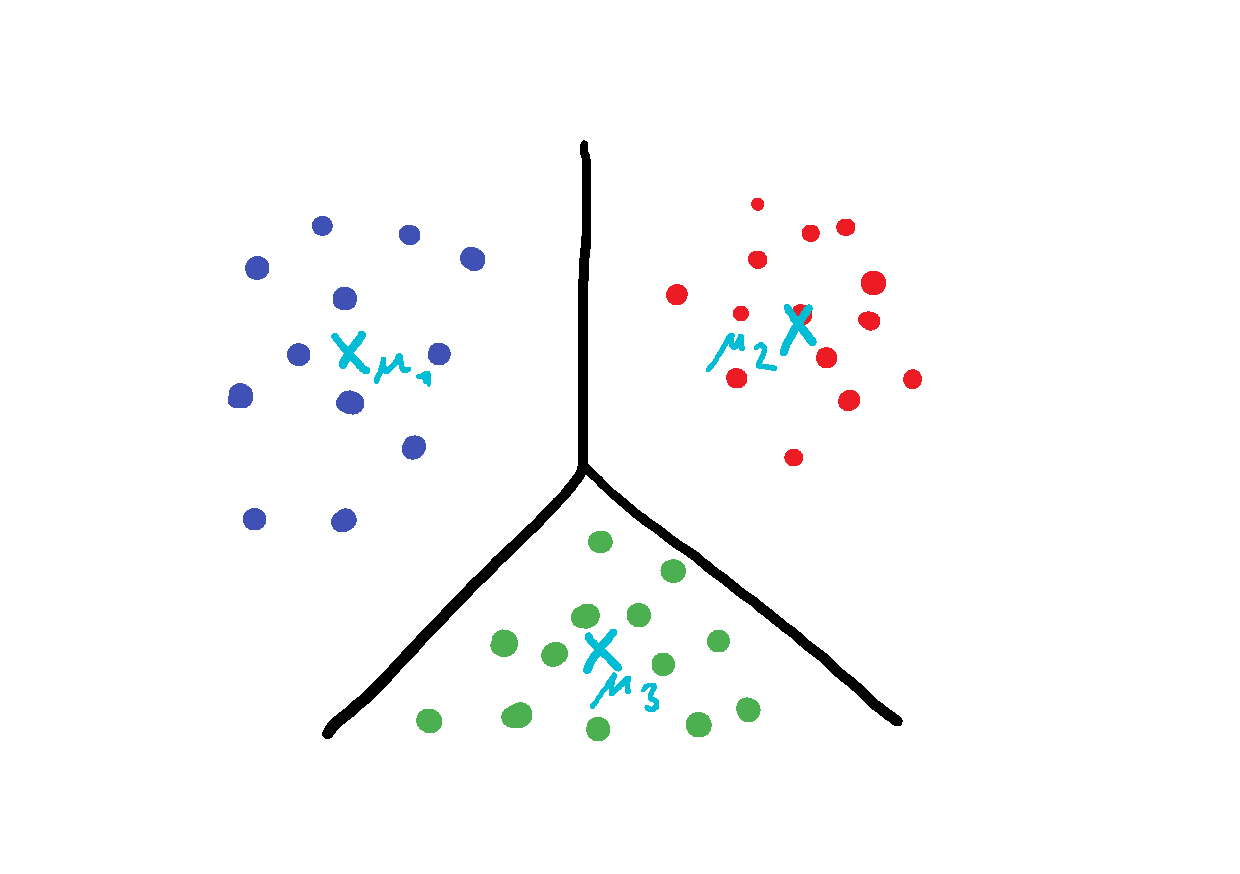
\includegraphics[height=5cm]{images/skizze_kmeans}
  \end{wrapfigure}
  \leavevmode
  \begin{itemize}
    \item Datenpunkte $\symbf{x_j}$ werden in $k$ \\ disjunkte Teilmengen $S_i$ partitioniert.
    \item Summierter quadratischer Fehler zu \\ Clusterzentren $\symbf{\mu_i}$ wird minnimiert
          \begin{equation*}
            \sum_{i=1}^{k} \sum_{\symbf{x_j} \in S_i} \lVert \symbf{x_j} - \symbf{\mu_i} \rVert^2 \rightarrow min.
          \end{equation*}
    \item Clusterzentren werden zunächst (zufällig) gewählt und dann iterativ aktualisiert.
  \end{itemize}
\end{frame}
% --- kmeans Clustering 1

% === Vorgehen

% === Experiment
\section{Erstes Experiment}

\begin{frame}{Übersicht}
  \tableofcontents[currentsection]
\end{frame}

% --- Experiment 1
\begin{frame}{Erstes Experiment}
  Die Kompressionseigenschaften der DCT und DWT werden an einem einfachen Beispiel untersucht.
  \begin{itemize}
    \item Gewichte einer Faltungsschicht eines trainierten CNNs werden komprimiert.
    \item Mehrere Filter werden als ein Vektor aufgefasst, um die Signallänge zu erhöhen.
    \item Diese werden jeweils mittels DCT bzw. DWT transformiert.
    \item Transformierte werden auf die ersten $n$ (DCT) bzw. betraglich größten $n$ (DWT) \\ Koeffizienten beschränkt.
    \item Transformationen werden invertiert.
          % \item Norm des Fehlers
          % \item erwarten bei gelicher Parameterzahl geringeren Fehler bei DWT
          % \item bei DWT eine geringe Auswahl von Konfigurationen (Wavelet/Tiefe)
  \end{itemize}
\end{frame}
% --- Experiment 1

% --- Experiment 2
\begin{frame}
  \begin{wrapfigure}{l}{8cm}
    \vspace{-0.8cm}
    \resizebox{7.8cm}{!}{%
      % This file was created with tikzplotlib v0.10.1.
\begin{tikzpicture}

\definecolor{darkgray176}{RGB}{176,176,176}
\definecolor{lightgray204}{RGB}{204,204,204}
\definecolor{steelblue31119180}{RGB}{31,119,180}

\begin{axis}[
legend style={fill opacity=0.8, draw opacity=1, text opacity=1, draw=lightgray204},
tick align=outside,
tick pos=left,
x grid style={darkgray176},
xlabel={\(\displaystyle t\)},
xmin=-1.15, xmax=2.15,
xtick style={color=black},
y grid style={darkgray176},
ylabel={\(\displaystyle \psi(t)\)},
ymin=-1.1, ymax=1.1,
ytick style={color=black}
]
\addplot [semithick, steelblue31119180, forget plot]
table {%
-1 0
-0.987951807228916 0
-0.975903614457831 0
-0.963855421686747 0
-0.951807228915663 0
-0.939759036144578 0
-0.927710843373494 0
-0.91566265060241 0
-0.903614457831325 0
-0.891566265060241 0
-0.879518072289157 0
-0.867469879518072 0
-0.855421686746988 0
-0.843373493975904 0
-0.831325301204819 0
-0.819277108433735 0
-0.807228915662651 0
-0.795180722891566 0
-0.783132530120482 0
-0.771084337349398 0
-0.759036144578313 0
-0.746987951807229 0
-0.734939759036145 0
-0.72289156626506 0
-0.710843373493976 0
-0.698795180722892 0
-0.686746987951807 0
-0.674698795180723 0
-0.662650602409639 0
-0.650602409638554 0
-0.63855421686747 0
-0.626506024096386 0
-0.614457831325301 0
-0.602409638554217 0
-0.590361445783133 0
-0.578313253012048 0
-0.566265060240964 0
-0.55421686746988 0
-0.542168674698795 0
-0.530120481927711 0
-0.518072289156627 0
-0.506024096385542 0
-0.493975903614458 0
-0.481927710843373 0
-0.469879518072289 0
-0.457831325301205 0
-0.44578313253012 0
-0.433734939759036 0
-0.421686746987952 0
-0.409638554216867 0
-0.397590361445783 0
-0.385542168674699 0
-0.373493975903614 0
-0.36144578313253 0
-0.349397590361446 0
-0.337349397590361 0
-0.325301204819277 0
-0.313253012048193 0
-0.301204819277108 0
-0.289156626506024 0
-0.27710843373494 0
-0.265060240963855 0
-0.253012048192771 0
-0.240963855421687 0
-0.228915662650602 0
-0.216867469879518 0
-0.204819277108434 0
-0.192771084337349 0
-0.180722891566265 0
-0.168674698795181 0
-0.156626506024096 0
-0.144578313253012 0
-0.132530120481928 0
-0.120481927710843 0
-0.108433734939759 0
-0.0963855421686747 0
-0.0843373493975903 0
-0.0722891566265059 0
-0.0602409638554217 0
-0.0481927710843373 0
-0.036144578313253 0
-0.0240963855421686 0
-0.0120481927710843 0
0 1
0.0120481927710845 1
0.0240963855421688 1
0.036144578313253 1
0.0481927710843375 1
0.0602409638554218 1
0.072289156626506 1
0.0843373493975905 1
0.0963855421686748 1
0.108433734939759 1
0.120481927710844 1
0.132530120481928 1
0.144578313253012 1
0.156626506024097 1
0.168674698795181 1
0.180722891566265 1
0.192771084337349 1
0.204819277108434 1
0.216867469879518 1
0.228915662650602 1
0.240963855421687 1
0.253012048192771 1
0.265060240963855 1
0.27710843373494 1
0.289156626506024 1
0.301204819277108 1
0.313253012048193 1
0.325301204819277 1
0.337349397590361 1
0.349397590361446 1
0.36144578313253 1
0.373493975903614 1
0.385542168674699 1
0.397590361445783 1
0.409638554216867 1
0.421686746987952 1
0.433734939759036 1
0.44578313253012 1
0.457831325301205 1
0.469879518072289 1
0.481927710843373 1
0.493975903614458 1
0.506024096385542 -1
0.518072289156627 -1
0.530120481927711 -1
0.542168674698795 -1
0.55421686746988 -1
0.566265060240964 -1
0.578313253012048 -1
0.590361445783133 -1
0.602409638554217 -1
0.614457831325301 -1
0.626506024096386 -1
0.63855421686747 -1
0.650602409638554 -1
0.662650602409639 -1
0.674698795180723 -1
0.686746987951807 -1
0.698795180722892 -1
0.710843373493976 -1
0.72289156626506 -1
0.734939759036145 -1
0.746987951807229 -1
0.759036144578313 -1
0.771084337349398 -1
0.783132530120482 -1
0.795180722891566 -1
0.807228915662651 -1
0.819277108433735 -1
0.831325301204819 -1
0.843373493975904 -1
0.855421686746988 -1
0.867469879518072 -1
0.879518072289157 -1
0.891566265060241 -1
0.903614457831325 -1
0.91566265060241 -1
0.927710843373494 -1
0.939759036144578 -1
0.951807228915663 -1
0.963855421686747 -1
0.975903614457831 -1
0.987951807228916 -1
1 0
1.01204819277108 0
1.02409638554217 0
1.03614457831325 0
1.04819277108434 0
1.06024096385542 0
1.07228915662651 0
1.08433734939759 0
1.09638554216868 0
1.10843373493976 0
1.12048192771084 0
1.13253012048193 0
1.14457831325301 0
1.1566265060241 0
1.16867469879518 0
1.18072289156627 0
1.19277108433735 0
1.20481927710843 0
1.21686746987952 0
1.2289156626506 0
1.24096385542169 0
1.25301204819277 0
1.26506024096386 0
1.27710843373494 0
1.28915662650602 0
1.30120481927711 0
1.31325301204819 0
1.32530120481928 0
1.33734939759036 0
1.34939759036145 0
1.36144578313253 0
1.37349397590361 0
1.3855421686747 0
1.39759036144578 0
1.40963855421687 0
1.42168674698795 0
1.43373493975904 0
1.44578313253012 0
1.4578313253012 0
1.46987951807229 0
1.48192771084337 0
1.49397590361446 0
1.50602409638554 0
1.51807228915663 0
1.53012048192771 0
1.5421686746988 0
1.55421686746988 0
1.56626506024096 0
1.57831325301205 0
1.59036144578313 0
1.60240963855422 0
1.6144578313253 0
1.62650602409639 0
1.63855421686747 0
1.65060240963855 0
1.66265060240964 0
1.67469879518072 0
1.68674698795181 0
1.69879518072289 0
1.71084337349398 0
1.72289156626506 0
1.73493975903614 0
1.74698795180723 0
1.75903614457831 0
1.7710843373494 0
1.78313253012048 0
1.79518072289157 0
1.80722891566265 0
1.81927710843373 0
1.83132530120482 0
1.8433734939759 0
1.85542168674699 0
1.86746987951807 0
1.87951807228916 0
1.89156626506024 0
1.90361445783133 0
1.91566265060241 0
1.92771084337349 0
1.93975903614458 0
1.95180722891566 0
1.96385542168675 0
1.97590361445783 0
1.98795180722892 0
2 0
};
\end{axis}

\end{tikzpicture}

    }
  \end{wrapfigure}
  \leavevmode
  \begin{itemize}
    \item Gewichte $W$ einer Faltungsschicht \\ aus einem ResNet18
    \item 512 Filter der Größe $3 \times 3$
    \item Gruppierung von jeweils \\ 4 Filtern zu 128 Vektoren der \\ Länge 36
    \item Haar Wavelet für die DWT
    \item Nur 2 Subbänder $a_0$ und $d_0$ (Level 1)
  \end{itemize}
\end{frame}
% --- Experiment 2

% --- Experiment 3
\begin{frame}
  \begin{wrapfigure}{l}{8cm}
    \vspace{-0.8cm}
    \resizebox{7.8cm}{!}{%
      % This file was created with tikzplotlib v0.10.1.
\begin{tikzpicture}

\definecolor{darkgray176}{RGB}{176,176,176}
\definecolor{darkorange25512714}{RGB}{255,127,14}
\definecolor{lightgray204}{RGB}{204,204,204}
\definecolor{steelblue31119180}{RGB}{31,119,180}

\begin{axis}[
legend cell align={left},
legend style={
  fill opacity=0.8,
  draw opacity=1,
  text opacity=1,
  at={(0.97,0.03)},
  anchor=south east,
  draw=lightgray204
},
tick align=outside,
tick pos=left,
x grid style={darkgray176},
xlabel={Kompressionsfaktor},
xmin=0.6, xmax=9.4,
xtick style={color=black},
y grid style={darkgray176},
ylabel={Normalisierter Fehler 
 \(\displaystyle e_{rel}\)},
ymin=-0.046607475585386, ymax=0.978758379632833,
ytick style={color=black}
]
\addplot [semithick, steelblue31119180]
table {%
9 0.932150840759277
7.2 0.92421692609787
5.14285714285714 0.891453623771667
4 0.866038143634796
3.6 0.864060819149017
3 0.849342465400696
2.57142857142857 0.815710723400116
2.4 0.806412398815155
2.11764705882353 0.783090651035309
1.89473684210526 0.691582381725311
1.8 0.661345958709717
1.63636363636364 0.639122068881989
1.5 0.599117159843445
1.44 0.576391458511353
1.33333333333333 0.547637343406677
1.24137931034483 0.51213526725769
1.2 0.476507186889648
1.125 0.381945371627808
1.05882352941176 0.326091170310974
1 1.37568136437949e-07
};
\addlegendentry{DCT}
\addplot [semithick, darkorange25512714]
table {%
9 0.731678664684296
7.2 0.683795571327209
5.14285714285714 0.598288714885712
4 0.523815393447876
3.6 0.48941370844841
3 0.425979554653168
2.57142857142857 0.369816660881042
2.4 0.343426793813705
2.11764705882353 0.2943035364151
1.89473684210526 0.248749569058418
1.8 0.227121189236641
1.63636363636364 0.186587646603584
1.5 0.148958936333656
1.44 0.131311669945717
1.33333333333333 0.0975319966673851
1.24137931034483 0.0674435645341873
1.2 0.0545677915215492
1.125 0.0312185026705265
1.05882352941176 0.0139471152797341
1 6.32881693718446e-08
};
\addlegendentry{DWT [Haar; Level=1]}
\end{axis}

\end{tikzpicture}

    }
  \end{wrapfigure}
  \leavevmode
  \begin{itemize}
    \item $dct(W; n)$ ist DCT Transformierte \\ mit ersten n Koeffizienten
    \item $dwt(W; n)$ ist DWT Transformierte \\ mit betraglich n größten \\ Koeffizienten
    \item $e_{\mathcal{T}}(n) = W - \mathcal{T}^{-1}(\mathcal{T}(W; n))$
          % \item $e_{dwt}(n) = W - idwt(dwt(W; n))$
    \item $e_{rel}(n) = \frac{\lVert e_{\mathcal{T}}(n) \rVert}{\lVert W \rVert}$
  \end{itemize}
\end{frame}
% --- Experiment 3
% === Experiment

% === Ausblick
\section{Ausblick}

\begin{frame}{Ausblick}
  \tableofcontents[currentsection]
\end{frame}

% --- Ausblick 1
\begin{frame}{Ausblick}
  Neben den in der Motivation genannten Punkten sollen folgende Fragestellungen untersucht werden:
  \begin{itemize}
    \item Wie führt man das komprimierte Netz auf der Zielplattform aus?
          \begin{itemize}
            \item Die Rücktransformation aller Schichten zur selben Zeit ist nicht sinnvoll.
            \item Gewichte können schichtweise rekonstruiert werden.
          \end{itemize}
    \item Wie werden sinnvolle Parameter (z.B. $k$ in $k$-Means) identifiziert?
    \item Können verschiedene Schichten sinnvoll gemeinsam geclustert werden?
  \end{itemize}
\end{frame}
% --- Ausblick 1

% === Ausblick
\end{document}
